\documentclass[12pt]{article}
\usepackage[margin=1in]{geometry}
\usepackage[table]{xcolor}    %for shading*
\usepackage{fullpage}
\usepackage{natbib}
\usepackage{mathpazo}
\usepackage{tipa}
\usepackage{setspace}
\usepackage{amsmath}
\usepackage{linguex}
\usepackage{tikz}
\usetikzlibrary{matrix,arrows}
\usepackage{tkz-euclide}
\usetkzobj{all}
\usepackage{slashbox}	
\usepackage{pifont}    %for pointing hand
\usepackage{arydshln}  %for dashed lines
\usepackage{rotating}  %for angled text
\usepackage{wasysym}   %for frowny face
\usepackage{amssymb} % for angle symbol
\usepackage{longtable}
\usepackage{amsfonts}
\newcommand{\tickYes}{\checkmark}
\usepackage{pifont}
\newcommand{\tickNo}{\hspace{1pt}\ding{55}}


\usepackage{fixltx2e}

%\makeatletter
%\newcommand\textsubscript[1]{\@textsubscript{\selectfont#1}}
%\def\@textsubscript#1{{\m@th\ensuremath{_{\mbox{\fontsize\sf@size\z@#1}}}}}
\newcommand{\iep}{\textipa{1}}
\newcommand{\bet}{\textipa{B}}
\newcommand{\schwa}{\textipa{@}}

\newsavebox{\sonorityanglehierarchycompressed}
\savebox{\sonorityanglehierarchycompressed}{
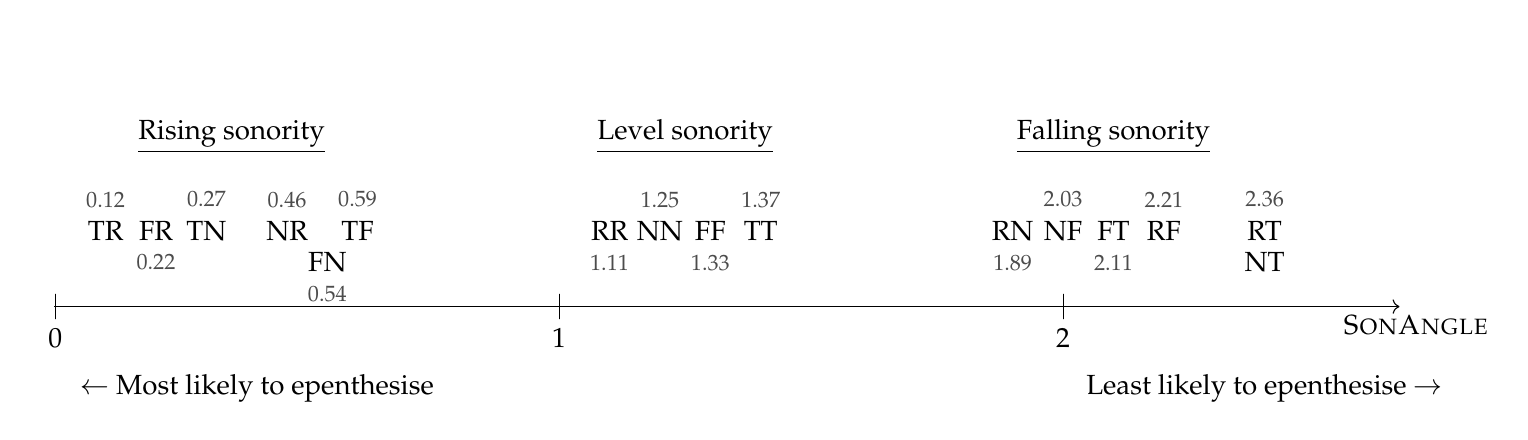
\begin{tikzpicture}[scale=0.8,shorten >=1pt,->]
  \tikzstyle{vertex}=[circle]
  \tikzstyle{point}=[circle,fill=black!25,minimum size=12pt,inner sep=2pt]
  \tikzstyle{line} = [draw, -latex']
  \node[vertex] (RT) at (2.4*8,1)   {RT};
  \node[vertex] (NT) at (2.4*8,0.5)  {NT};
  \node[vertex] (FT) at (2.1*8,1)  {FT};
  \node[vertex] (TT) at (1.4*8,1)     {TT};
  \node[vertex] (RF) at (2.2*8,1)     {RF};
  \node[vertex] (NF) at (2.0*8,1)  {NF};
  \node[vertex] (TF) at (0.6*8,1)   {TF};
  \node[vertex] (FF) at (1.3*8,1)   {FF};
  \node[vertex] (RN) at (1.9*8,1)   {RN};
  \node[vertex] (NN) at (1.2*8,1)   {NN};
  \node[vertex] (FN) at (0.54*8,0.5)  {FN};
  \node[vertex] (TN) at (0.3*8,1)   {TN};
  \node[vertex] (RR) at (1.1*8,1)  {RR};
  \node[vertex] (NR) at (0.46*8,1.0)  {NR};
  \node[vertex] (FR) at (0.2*8,1)   {FR};
  \node[vertex] (TR) at (0.1*8,1)   {TR};
  \node[vertex] (rising) at (0.35*8,2.5) {\underline{Rising sonority}};
  \node[vertex] (level) at (1.25*8,2.5) {\underline{Level sonority}};
  \node[vertex] (falling) at (2.1*8,2.5) {\underline{Falling sonority}};
  % axis
  \node[vertex] (axisstart) at (-0.23,-0.2) {};
  \node[vertex] (axisend)   at (2.7*8,-0.2) {};
  \draw (axisstart) -- (axisend);
  \draw (0.0*8, 0) -- (0.0*8, -0.4) -- cycle;
  \draw (1.0*8, 0) -- (1.0*8, -0.4) -- cycle;
  \draw (2.0*8, 0) -- (2.0*8, -0.4) -- cycle;
  \node[vertex] (0pointlabel) at (0.0,-0.7) {0};
  \node[vertex] (1pointlabel) at (1.0*8,-0.7) {1};
  \node[vertex] (2pointlabel) at (2.0*8,-0.7) {2};
  \node[vertex] (xaxislabel) at (2.7*8,-0.5) {\textsc{SonAngle}};
  \node (leastlikely) at (2.4*8,-1.5) {Least likely to epenthesise $\rightarrow$};
  \node (mostlikely) at (0.4*8,-1.5) {$\leftarrow$ Most likely to epenthesise};
  % numbers
  \node[font=\footnotesize,opacity=0.7] (RTno) at (2.4*8, 1.5) {2.36};
  \node[font=\footnotesize,opacity=0.7] (RFno) at (2.2*8, 1.5) {2.21};
  \node[font=\footnotesize,opacity=0.7] (FTno) at (2.1*8, 0.5) {2.11};
  \node[font=\footnotesize,opacity=0.7] (NFno) at (2.0*8, 1.5) {2.03};
  \node[font=\footnotesize,opacity=0.7] (RNno) at (1.9*8, 0.5) {1.89};

  \node[font=\footnotesize,opacity=0.7] (TTno) at (1.4*8, 1.5) {1.37};
  \node[font=\footnotesize,opacity=0.7] (FFno) at (1.3*8, 0.5) {1.33};
  \node[font=\footnotesize,opacity=0.7] (NNno) at (1.2*8, 1.5) {1.25};
  \node[font=\footnotesize,opacity=0.7] (RRno) at (1.1*8, 0.5) {1.11};

  \node[font=\footnotesize,opacity=0.7] (TFno) at (0.6*8, 1.5) {0.59};
  \node[font=\footnotesize,opacity=0.7] (FNno) at (0.54*8, 0) {0.54};
  \node[font=\footnotesize,opacity=0.7] (NRno) at (0.46*8, 1.5) {0.46};
  \node[font=\footnotesize,opacity=0.7] (TNno) at (0.3*8, 1.5) {0.27};
  \node[font=\footnotesize,opacity=0.7] (FRno) at (0.2*8, 0.5) {0.22};
  \node[font=\footnotesize,opacity=0.7] (TRno) at (0.1*8, 1.5) {0.12};

\end{tikzpicture}
}

\newsavebox{\sonorityrisehierarchycompressed}
\savebox{\sonorityrisehierarchycompressed}{
\begin{tikzpicture}[scale=0.8,shorten >=1pt,->]
  \tikzstyle{vertex}=[circle]
  \tikzstyle{point}=[circle,fill=black!25,minimum size=12pt,inner sep=2pt]
  \tikzstyle{line} = [draw, -latex']
  \node[vertex] (RT) at (2.5*8, 0)  {RT};
  \node[vertex] (NT) at (1.67*8,0)  {NT};
  \node[vertex] (FT) at (1.25*8,0)  {FT};
  \node[vertex] (TT) at (1*8,-0.5)     {TT};
  \node[vertex] (RF) at (2*8,0)     {RF};
  \node[vertex] (NF) at (1.33*8,-0.5)  {NF};
  \node[vertex] (FF) at (1*8,0)   {FF};
  \node[vertex] (TF) at (0.8*8,-0.5)   {TF};
  \node[vertex] (RN) at (1.5*8,0)   {RN};
  \node[vertex] (NN) at (1*8,0.5)     {NN};
  \node[vertex] (FN) at (0.75*8,0)  {FN};
  \node[vertex] (TN) at (0.6*8,0)   {TN};
  \node[vertex] (RR) at (1*8,1.0)  {RR};
  \node[vertex] (NR) at (0.67*8,-0.5)  {NR};
  \node[vertex] (FR) at (0.5*8,0)   {FR};
  \node[vertex] (TR) at (0.4*8,0)   {TR};
  \node[vertex] (rising) at (0.5*8,2) {\underline{Rising sonority}};
  \node[vertex] (level) at (1*8,2) {\underline{Level sonority}};
  \node[vertex] (falling) at (1.67*8,2) {\underline{Falling sonority}};
  % axis
  \node[vertex] (axisstart) at (-0.23,-1.0) {};
  \node[vertex] (axisend)   at (2.7*8,-1.0) {};
  \draw (axisstart) -- (axisend);
  \draw (0.0*8, -1.2) -- (0.0*8, -0.8) -- cycle;
  \draw (1.0*8, -1.2) -- (1.0*8, -0.8) -- cycle;
  \draw (2.0*8, -1.2) -- (2.0*8, -0.8) -- cycle;
  \node[vertex] (0pointlabel) at (0.0,-1.5) {0};
  \node[vertex] (1pointlabel) at (1.0*8,-1.5) {1};
  \node[vertex] (2pointlabel) at (2.0*8,-1.5) {2};
  \node[vertex] (xaxislabel) at (2.7*8,-1.5) {\textsc{SonRise}};
\end{tikzpicture}
}

\newsavebox{\syllablecontacthierarchy}
\savebox{\syllablecontacthierarchy}{
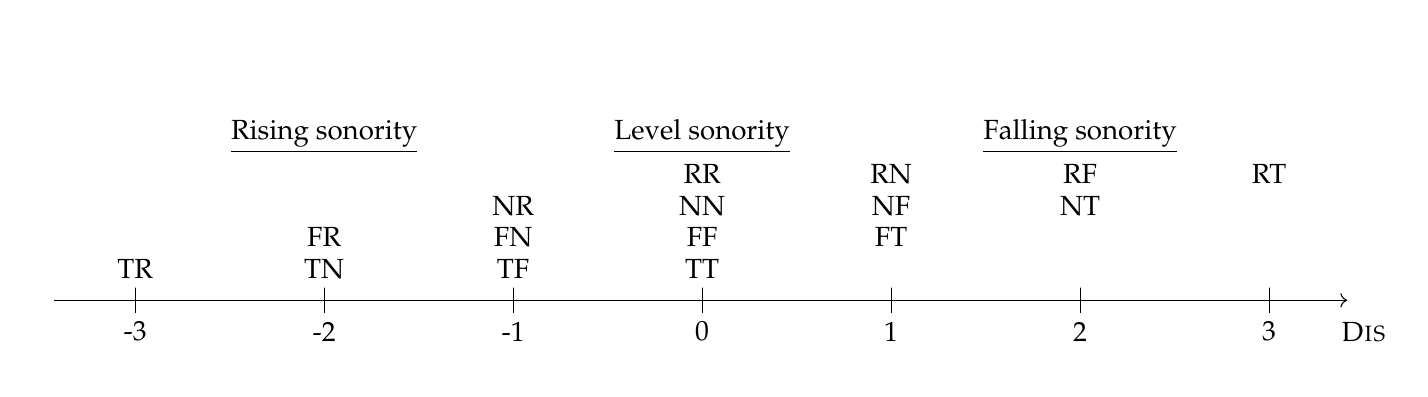
\begin{tikzpicture}[scale=0.8,shorten >=1pt,->]
  \tikzstyle{vertex}=[circle]
  \tikzstyle{point}=[circle,fill=black!25,minimum size=12pt,inner sep=2pt]
  \tikzstyle{line} = [draw, -latex']
  \node[vertex] (RT) at (3*3,2.0)   {RT};
  \node[vertex] (NT) at (2*3,1.5)  {NT};
  \node[vertex] (FT) at (1*3,1.0)  {FT};
  \node[vertex] (TT) at (0*3,0.5)     {TT};
  \node[vertex] (RF) at (2*3,2.0)     {RF};
  \node[vertex] (NF) at (1*3,1.5)  {NF};
  \node[vertex] (FF) at (0*3,1.0)   {FF};
  \node[vertex] (TF) at (-1*3,0.5)   {TF};
  \node[vertex] (RN) at (1*3,2.0)   {RN};
  \node[vertex] (NN) at (0*3,1.5)   {NN};
  \node[vertex] (FN) at (-1*3,1)  {FN};
  \node[vertex] (TN) at (-2*3,0.5)   {TN};
  \node[vertex] (RR) at (0*3,2.0)  {RR};
  \node[vertex] (NR) at (-1*3,1.5)  {NR};
  \node[vertex] (FR) at (-2*3,1.0)   {FR};
  \node[vertex] (TR) at (-3*3,0.5)   {TR};
  % headers
  \node[vertex] (rising) at (2*3,2.6) {\underline{Falling sonority}};
  \node[vertex] (level) at (0*3,2.6) {\underline{Level sonority}};
  \node[vertex] (falling) at (-2*3,2.6) {\underline{Rising sonority}};
  % axis
  \node[vertex] (axisstart) at (-3.5*3,-0) {};
  \node[vertex] (axisend)   at (3.5*3,-0) {};
  \draw (axisstart) -- (axisend);
  \draw (0, 0.2) -- (0, -0.2) -- cycle;
  \draw (1*3, 0.2) -- (1*3, -0.2) -- cycle;
  \draw (2*3, 0.2) -- (2*3, -0.2) -- cycle;
  \draw (3*3, 0.2) -- (3*3, -0.2) -- cycle;
  \draw (-1*3, 0.2) -- (-1*3, -0.2) -- cycle;
  \draw (-2*3, 0.2) -- (-2*3, -0.2) -- cycle;
  \draw (-3*3, 0.2) -- (-3*3, -0.2) -- cycle;
  \node[vertex] (0pointlabel) at (0.0,-0.5) {0};
  \node[vertex] (1pointlabel) at (1.0*3,-0.5) {1};
  \node[vertex] (2pointlabel) at (2.0*3,-0.5) {2};
  \node[vertex] (3pointlabel) at (3.0*3,-0.5) {3};
  \node[vertex] (-1pointlabel) at (-1.0*3,-0.5) {-1};
  \node[vertex] (-2pointlabel) at (-2.0*3,-0.5) {-2};
  \node[vertex] (-3pointlabel) at (-3.0*3,-0.5) {-3};
  \node[vertex] (xaxislabel) at (3.5*3,-0.5) {\textsc{Dis}};
\end{tikzpicture}
}





\title{The perceptual dimensions of \\ sonority-driven epenthesis}
\author{Michelle A. Fullwood}
\date{Generals Paper, MIT \\ October 2013}
\begin{document}

\maketitle

\begin{abstract}
 
Vowel epenthesis often appears to preferentially target consonant clusters with rising sonority.
One explanation for this is perceptual faithfulness \citep{fleischhacker.2002,steriade.2006}: rising sonority clusters are more susceptible to epenthesis because the perceptual distance between the underlying /C\textsubscript{1}C\textsubscript{2}/ sequence and its correspondent output sequence [C\textsubscript{1}VC\textsubscript{2}] is small, thus incurring a smaller faithfulness cost.
This raises the question of how to compute the perceptual distance between two sonority contours /C\textsubscript{1}C\textsubscript{2}/ and [C\textsubscript{1}VC\textsubscript{2}] in terms of the sonority of C\textsubscript{1}, C\textsubscript{2} and V.  
In this paper, I propose two desiderata for such a metric, and propose a metric that fits these considerations --- {\sc Sonority Angle}, the angle formed by the contours C\textsubscript{1}C\textsubscript{2} and C\textsubscript{1}V. I apply it in analyzing two case studies of sonority-driven epenthesis, Chaha and Irish.  A comparison is made to another possible metric,
{\sc Sonority Rise} \citep{flemming.2008}, the ratio of the gradients of the two contours, as well as to Syllable Contact and Sonority Sequencing, which represent an alternative, markedness-based approach to the problem of sonority-driven epenthesis. 
\end{abstract}

\newpage
\tableofcontents
\newpage

\section{Introduction}

Vowel epenthesis often appears to preferentially target consonant clusters with rising sonority, as in the following example of English loanwords borrowed into Hawai'ian creole. The rising sonority onset cluster is adapted with epenthesis, while the falling sonority cluster is left intact.

\ex. \a. puranti: `plenty'
    \b. ste: `stay'
    \z.
    (\cite{nagara.1972}, cited by \cite{fleischhacker.2005})

There are two broad classes of explanation within Optimality Theory for such sonority-driven epenthesis.

One is faithfulness-based: the perceptual distance between the underlying /C\textsubscript{1}C\textsubscript{2}/ sequence and its correspondent
output sequence [C\textsubscript{1}VC\textsubscript{2}] is small when the cluster is of rising sonority.
Thus, epenthesis into such a sequence incurs a smaller faithfulness cost than epenthesis into a cluster of falling sonority. This is the basis of the analysis proposed by \cite{fleischhacker.2002, fleischhacker.2005} to explain why rising sonority obstruent-sonorant clusters are more easily epenthesised in
to than falling sonority sibilant-stop clusters.

This raises the question of how the perceptual distance between two sonority contours /C\textsubscript{1}C\textsubscript{2}/ and [C\textsubscript{1}VC\textsubscript{2}] should be computed in terms of the sonority of C\textsubscript{1}, C\textsubscript{2} and V.  

Fleischhacker's analysis rested on empirical determinations of sonority contour faithfulness of specific clusters such as stop-liquid (TR) clusters and fricative-stop (FT) clusters, and did not attempt to determine a formula for arbitrary values of C\textsubscript{1}, C\textsubscript{2}. \citet{steriade.2006} proposed that input and output sonority contours should match in terms of whether they are rising or falling, and to what degree, but did not suggest a concrete mathematical relation.  \citet{flemming.2008} formalises Steriade's approach with the metric {\sc Sonority Rise}, the ratio of the gradients of the two contours.

\bigskip

In this paper, I suggest that any such metric should bear two properties. The first is suggested by previous analyses, while the second is original to this paper.

\ex. Desiderata for a sonority contour faithfulness metric \label{desiderata}
     \a. The more positive the gradient of the sonority contour from C\textsubscript{1} to C\textsubscript{2}, the smaller the faithfulness cost. \label{desideratum_a}
     \b. For a given sonority distance between C\textsubscript{1} and C\textsubscript{2}, the more sonorous C\textsubscript{1} and C\textsubscript{2} are, the smaller the faithfulness cost. \label{desideratum_b}

To make things concrete, I suggest a metric that possesses these two properties, which I term {\sc Sonority Angle}. This is the magnitude of the angle made by the vectors C\textsubscript{1}C\textsubscript{2} and C\textsubscript{1}V. I then explore the ramifications of this choice. 

{\sc Sonority Angle} makes the same broad predictions as {\sc Sonority Rise} --- that clusters of rising sonority, having a relatively small angle between the underlying sonority contour /C\textsubscript{1}C\textsubscript{2}/ and the overt sonority contour [C\textsubscript{1}V], are perceptually more similar to their epenthetic output, and therefore more likely to undergo epenthesis, than clusters of falling sonority. Crucially, however, the exact hierarchy of susceptibility of individual clusters to epenthesis is predicted to be different.

I take two instances where the predictions of {\sc Sonority Angle} and {\sc Sonority Rise} differ and illustrate with case studies of sonority-driven epenthesis in two different languages, namely Chaha and Irish, that the predictions of {\sc Sonority Angle} are more in line with the data than those of {\sc Sonority Rise}.

\bigskip

The other broad class of explanation for sonority-driven epenthesis is markedness-based.  Syllable Contact \citep{murray.vennemann.1983} holds that across a syllable boundary, falling sonority clusters are more harmonic than rising sonority ones.  Hence, rising sonority clusters are preferentially broken up by epenthesis.

Syllable Contact forms the basis for the main existing analysis of Chaha epenthesis by \citet{rose.2000}.  I show that the faithfulness-based analysis, powered by the metric of {\sc Sonority Angle}, is equally capable of explaining the Chaha facts. Furthermore, in the case of Irish, Syllable Contact makes incorrect predictions regarding the data.

\bigskip

The layout of this paper is as follows.  Section \ref{theoreticalmachinery} lays out the theoretical background for the sonority contour faithfulness approach to 
sonority-driven epenthesis. I introduce the proposed {\sc Sonority Angle} metric as well as the competing {\sc Sonority Rise} metric \citep{flemming.2008}, 
then lay out the alternative markedness-based approach to sonority-driven epenthesis.

Section \ref{irish} consists of a case study of sonority-driven epenthesis in Irish.  I show that the data are in line with the predictions of {\sc Sonority Angle} and not {\sc Sonority Rise}, while a Syllable Contact-based analysis would have to be very complicated to explain the same facts.

Section \ref{chaha} is a case study of epenthesis positioning in Chaha.  I detail the facts of epenthesis positioning in Chaha, based on data from \cite{rose.2000},
and show that the sonority contour faithfulness approach explains these facts, with {\sc Sonority Angle} as the metric for comparing sonority contours.  I compare it to {\sc Sonority Rise} and show that the former is the more successful analysis, and that overall, the approach just outlined is comparably successful to the Syllable Contact-based approach of \citet{rose.2000}.

Section \ref{issues} discusses various issues regarding {\sc Sonority Angle}, such as its robustness. Section \ref{conclusion} concludes.

\section{Theoretical background} \label{theoreticalmachinery}

This paper assumes as its basis the P-map hypothesis \citep{steriade.2001}, which states that the perceptual distance between underlying representations and potential surface forms projects a fixed ranking of faithfulness constraints.

In order to determine what faithfulness constraints exist in {\sc Con} and what their rankings should be, therefore, we need to know the metrics of perceptual distance that are relevant to each change. In the case of vowel epenthesis, the perceptual distance to be measured is between two sonority contours, /C\textsubscript{1}C\textsubscript{2}/ and [C\textsubscript{1}VC\textsubscript{2}].

\subsection{Sonority Angle}

The first desideratum with which we started was that the more steeply rising the sonority profile of a consonant cluster, the more likely the cluster to undergo epenthesis. Thus the absolute difference in sonority between C\textsubscript{1} and C\textsubscript{2} must be factored into the metric. To this, I add the claim that the more sonorous C\textsubscript{1}, the more likely the cluster is to undergo epenthesis.

These two criteria are fulfilled by the metric {\sc Sonority Angle}, which is defined as the angle between the underlying C\textsubscript{1}C\textsubscript{2} sonority contour and the surface C\textsubscript{1}V contour:

\ex. Visual representation of {\sc Sonority Angle} \label{sonangle_picture} 

\vspace{-3em}
\begin{center}
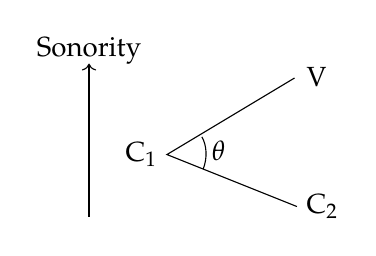
\begin{tikzpicture} [shorten >=1pt,scale=0.33]
                      \draw [<-] (-3,6.5) -- (-3, 0.5) ; % axis
                      \node at (-3, 7.0) {Sonority}; % axis label
                      \draw (5,1) -- (0,3) -- (5,6) ; % rising sonority
%                      \node at (1.8, 3.2) {$\theta$}; % theta label for rising sonority
                      \node[left] at (0,3) {C$_1$}; 
                      \node[right] at (5,1) {C$_2$};
                      \node[right] at (5,6) {V};
    \coordinate (A) at (0,3);
    \coordinate (B) at (5,1);
    \coordinate (C) at (5,6);
\tkzMarkAngle[size=1.5cm](B,A,C)
\tkzLabelAngle[pos=2](B,A,C){$\theta$}
\end{tikzpicture} 
\end{center}

Assuming that the horizontal distance is 1 unit, we can compute the magnitude of this angle analytically with the following formula:

\ex. \label{sonangle_formula} Formula: \textsc{SonAngle} = $arctan(V-C_1) - arctan(C_2-C_1)$

Let us verify that {\sc Sonority Angle} does indeed reflect the two generalisations we wish to make: first, that the smaller the sonority distance between C\textsubscript{1} and C\textsubscript{2}, the smaller the sonority angle.

\ex. Illustration: keeping C\textsubscript{1} fixed, raising the sonority of C\textsubscript{2} decreases the {\sc Sonority Angle}.

\vspace{-5em}
\begin{center}
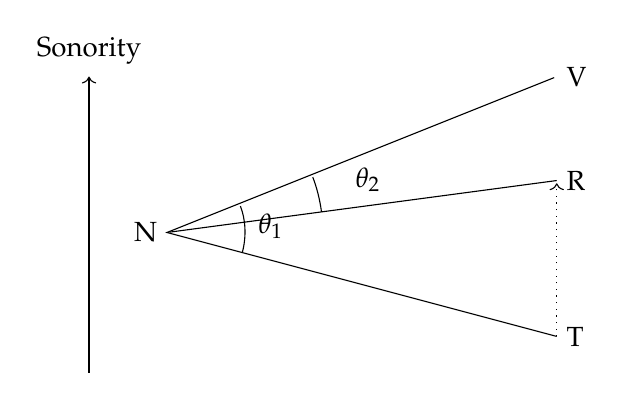
\begin{tikzpicture} [shorten >=1pt,scale=0.33]
                      \draw [<-] (-3,12) -- (-3, 0.5) ; % axis
                      \node at (-3, 13.0) {Sonority}; % axis label
					 % left diagram
    \coordinate (A) at (0,6); % pivot - C1
    \coordinate (B) at (15,2); % C2
    \coordinate (C) at (15,12); % V
    \draw (B) -- (A) -- (C);
	\tkzMarkAngle[size=3cm](B,A,C);
	\tkzLabelAngle[pos=4](B,A,C){$\theta_1$};
    \coordinate (D) at (15,8); % another C2
    \draw (D) -- (A);
	\tkzMarkAngle[size=6cm](D,A,C);
	\tkzLabelAngle[pos=8](D,A,C){$\theta_2$};
    
    \node[left] at  (A) {N}; 
    \node[right] at (B) {T};
    \node[right] at (C) {V};
    \node[right] at (D) {R};
    
    \draw [->,dotted] (B) -- (D);
\end{tikzpicture} 
\end{center}

The dependence of {\sc Sonority Angle} on this distance can also be seen in the second term in \ref{sonangle_formula}.

The second generalisation is that the more sonorous the C\textsubscript{1}, the more likely
epenthesis is to occur. Let us fix the sonority distance between the two consonants of the cluster at 2, but vary their distance from V. Decreasing this distance decreases the {\sc Sonority Angle}.

\ex. Illustration: keeping C\textsubscript{1} -- C\textsubscript{2} fixed at 1, raising the sonority in cluster decreases the {\sc Sonority Angle}.

\vspace{-9em}
\begin{center}
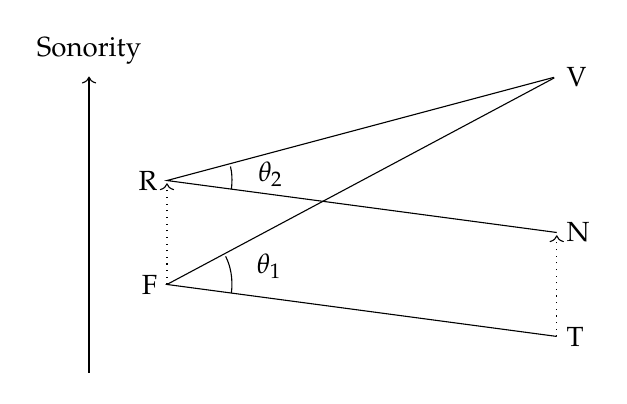
\begin{tikzpicture} [shorten >=1pt,scale=0.33]
                      \draw [<-] (-3,12) -- (-3, 0.5) ; % axis
                      \node at (-3, 13.0) {Sonority}; % axis label
					 % left diagram
    \coordinate (A) at (0,4); % pivot - C1 - F * 3
    \coordinate (B) at (15,2); % C2 - T * 3
    \coordinate (C) at (15,12); % V
    \draw (B) -- (A) -- (C);
	\tkzMarkAngle[size=2.5cm](B,A,C);
	\tkzLabelAngle[pos=4](B,A,C){$\theta_1$};
    \coordinate (D) at (15,6); % another C2 - N * 3
    \coordinate (E) at (0,8); % another C1 - R * 3
    \draw (D) -- (E) -- (C);
	\tkzMarkAngle[size=2.5cm](D,E,C);
	\tkzLabelAngle[pos=4](D,E,C){$\theta_2$};
    
    \node[left] at  (A) {F}; 
    \node[right] at (B) {T};
    \node[right] at (C) {V};
    \node[right] at (D) {N};
    \node[left] at (E) {R};   
    \draw [->,dotted] (B) -- (D);
    \draw [->,dotted] (A) -- (E);
\end{tikzpicture} 
\end{center}

The first term in formula \ref{sonangle_formula} confirms the relation between the sonority of C\textsubscript{1} in terms of its closeness to V, and {\sc Sonority Angle} as a whole.

\bigskip

Given a sonority scale where classes of consonants are mapped to a numerical sonority, we can now calculate the {\sc Sonority Angle} for any cluster, which can be thought of as the faithfulness cost of epenthesising between the two consonants.  Examples of the calculation are given below.

In this paper, I adopt (with, later, minor modifications) the following standard scale \citep[(10)]{flemming.2008}:

\ex. \label{standardsonorityscale} 
      \begin{tabular}{cccccc}
         T & F & N & R & G & V \\
         stop & fricative & nasal & liquid & glide & vowel \\
         1 & 2 & 3 & 4 & 5 & 6 \\
      \end{tabular}

The {\sc Sonority Angles} for NT, TT and TN are calculated as in the following examples.

\ex. \a. \textsc{SonAngle}(NT) =  $arctan(6-3) - arctan(1-3)$ = 2.35
     \b. \textsc{SonAngle}(TT) =  $arctan(6-1) - arctan(1-1)$ = 1.37
     \c. \textsc{SonAngle}(TN) =  $arctan(6-1) - arctan(3-1)$ = 0.27

The larger the {\sc Sonority Angle}, the larger the faithfulness cost. We therefore expect it to be hardest to epenthesise into NT out of these three clusters, and easiest to epenthesise into TN.

I formalise the idea of faithfulness cost by defining a family of \textsc{Ident} constraints that penalise outputs that incur faithfulness costs of greater than a certain $n$, following \cite{flemming.2008}.

\ex. \textsc{Ident(Son$\measuredangle$)}$<$n: Assign a violation mark if the consonants in two strings C\textsubscript{1}C\textsubscript{2} and C\textsubscript{1}VC\textsubscript{2} 
stand in correspondence, and the {\sc Sonority Angle} between C\textsubscript{1}C\textsubscript{2} and C\textsubscript{1}V is greater than $n$.

This family of faithfulness constraints forms a stringency hierarchy. Any cluster that would violate \textsc{Ident(Son$\measuredangle$)}$<$n, would also violate {\sc Ident(Son$\measuredangle$)}$<$m, where m$>$n.

The resulting hierarchy of clusters, ranked according to their resistance to epenthesis as defined
by their {\sc Sonority Angle}, is as follows.
	
\ex. {\sc Sonority Angle} hierarchy

\vspace{-3em}
\noindent \resizebox{\linewidth}{!}{\usebox{\sonorityanglehierarchycompressednumbers}}

The prediction is that when a markedness constraint targets a set of clusters for epenthesis, if a certain cluster undergoes epenthesis, then all clusters to the left of it on the hierarchy --- those with a smaller {\sc Sonority Angle} --- should also undergo epenthesis.

Notice that out of the falling sonority clusters, those that decrease in sonority by a single step
--- namely RN, NF and FT --- have smaller {\sc Sonority Angles} than the ones that have a greater fall
in sonority. Furthermore, out of these three clusters, the one with the most sonorous C\textsubscript{1}, RN, has the smallest {\sc Sonority Angle}. We thus predict that out of the falling sonority clusters, RN is the most likely to be broken up by epenthesis. The case study on Chaha will demonstrate that this is the case.

Similarly, between the clusters that fall in sonority by two steps --- RF and NT --- we expect
NT to be less likely to undergo epenthesis, since N is less sonorous than R. 

Among falling clusters that share the same C\textsubscript{2}, there is a tension between wanting a small sonority distance and wanting C\textsubscript{1} to have as high a sonority as possible. RT and NT resolve this in different ways, ending up with the same {\sc Sonority Angle}, which is the largest out of the all the clusters. We thus expect NT and RT to be the clusters most resistant to epenthesis out of all the clusters. This will be crucial to our analysis of Irish sonority-driven epenthesis.

\subsection{Stringency and faithfulness conflation}

There are two possible ways to rank the family of {\sc Ident(Son$\measuredangle$)}$<$n constraints.
One is to fix them in a universal ranking \citep{prince.smolensky.1993}, with the least stringent constraint the highest-ranked:

\ex. Universal ranking: \\
     {\sc Ident(Son$\measuredangle$)}$<$2.0 $\gg$ {\sc Ident(Son$\measuredangle$)}$<$1.5 $\gg$ ...

It is also possible to allow them to be freely ranked \citep[and others]{de.lacy.2004}, so that a more stringent constraint may outrank a less stringent one:

\ex. Possible free ranking: \label{freerankingex}
     {\sc Ident(Son$\measuredangle$)}$<$1.5 $\gg$ {\sc Ident(Son$\measuredangle$)}$<$2.0 $\gg$ ...

This represents a slight deviation from the P-map hypothesis \citep{steriade.2001} in implementation, though not in spirit. Because the constraints form a stringency hierarchy, there cannot be reversals of the cluster hierarchy. What may occur is the {\it conflation} of certain areas of the constraint hierarchy, such as all the clusters with {\sc Sonority Angles} between 1.5 and 2.0 in \ref{freerankingex}, depending on what constraints intervene. Some illustrative examples are given below.

\bigskip

In this paper, for ease of analysis, I will assume that all {\sc Ident(Son$\measuredangle$)}$<$n constraints are ranked low by default, but that individual {\sc Ident(Son$\measuredangle$)}$<$n constraints can be promoted to dominate a markedness constraint $\mathcal{M}$ against clusters or another faithfulness constraint $\mathcal{F}$, blocking epenthesis for all clusters with a {\sc Sonority Angle} greater than $n$, with the result that either the cluster remains intact, or a competing solution to epenthesis emerges.

An example of {\sc Ident(Son$\measuredangle$)}$<$n blocking epenthesis is given in the sample tableaux below.

\ex. Ident(Son$\measuredangle$)$<$1.5 $\gg$ {\sc *ComplexCoda} $\gg$ {\sc Dep}
     \a. Allows epenthesis in rising and level clusters such as stop-fricative TF:
\vspace{-0.5em}
\begin{center} \renewcommand*\arraystretch{1.2}
\scalebox{1}[1]{\begin{tabular}[t]{|rrl||c|c|c|} \hline 
\multicolumn{3}{|c||}{Input:~/TF/} & {\sc Ident(Son$\measuredangle$)}$<$1.5 & {\sc *ComplexCoda} & {\sc Dep} \\[0.5ex]
\hline \hline a. & & TF & & $\ast$! & \cellcolor{lightgray} \\
\hline b. & \ding{43} & T\textipa{@}F & 0.59 & & \cellcolor{lightgray}$\ast$ \\
\hline \end{tabular}} \renewcommand*\arraystretch{1} \end{center}
\vspace{0.5em}
     \b. Prevents epenthesis in falling clusters such as FT:
\vspace{-0.5em}
\begin{center} \renewcommand*\arraystretch{1.2}
\scalebox{1}[1]{\begin{tabular}[t]{|rrl||c|c|c|} \hline 
\multicolumn{3}{|c||}{Input:~/FT/} & {\sc Ident(Son$\measuredangle$)}$<$1.5 & {\sc *ComplexCoda} & {\sc Dep} \\[0.5ex]
\hline \hline c. & \ding{43} & FT & &\cellcolor{lightgray} $\ast$ & \cellcolor{lightgray} \\
\hline d. & & F\textipa{@}T & 2.11 $\ast$! &\cellcolor{lightgray} & \cellcolor{lightgray}$\ast$ \\
\hline \end{tabular}} \renewcommand*\arraystretch{1} \end{center}

We will see more examples of this in the analysis of Irish epenthesis as well as Chaha coda cluster epenthesis.

\bigskip       

I will illustrate the use of {\sc Ident(Son$\measuredangle$)}$<$n to block epenthesis in favour of other cluster resolution strategies with an example from the loanword phonology of the Dhaka dialect of Bangla, which is discussed and given an alternative analysis in \citep{karim.2011}. Standard Bangla keeps coda clusters in words borrowed from English, but these are simplified in the Dhaka dialect in a variety of ways, including both epenthesis and deletion of one of the consonants in the cluster.  

\ex. \a. RN clusters are broken up via copy epenthesis \label{banglaRN}
         \a. \textipa{hOrn} $\rightarrow$ \textipa{hOrOn} `horn'
         \b. \textipa{p\textsuperscript{h}Orm} $\rightarrow$ \textipa{p\textsuperscript{h}OrOm} `form'
         \c. \textipa{fIlm} $\rightarrow$ \textipa{fIlIm} `film'
         \z.
     \b. RT clusters resolved by deletion of [r] \label{banglaRT}
         \a. \textipa{park} $\rightarrow$ \textipa{pak} `park'
         \b. \textipa{\textrtailt Orc} $\rightarrow$ \textipa{\textrtailt Oc} `torch'
         \c. \textipa{narb\textsuperscript{h}} $\rightarrow$ \textipa{nab\textsuperscript{h}} `nerve'
         \z.
     \citep[(4,5)]{karim.2011}

From the examples in \ref{banglaRN}, we see that {\sc Max}(r) $\gg$ {\sc Dep} in general, making epenthesis the preferred way of dealing with the cluster.

\ex. {\sc *ComplexCoda} $\gg$ {\sc Max}(r) $\gg$ {\sc Dep}
\vspace{-1em}
\begin{center} \renewcommand*\arraystretch{1.2}
\scalebox{1}[1]{\begin{tabular}[t]{|rrl||c:c|c|} \hline 
\multicolumn{3}{|c||}{Input:~/\textipa{hOrn}/} & {\sc *ComplexCoda} & {\sc Max}(r) & {\sc Dep} \\[0.5ex]
\hline \hline a. & & \textipa{hOrn} & $\ast$! & & \cellcolor{lightgray} \\
\hline b. & \ding{43} & \textipa{hOrOn} & & & \cellcolor{lightgray}$\ast$ \\
\hline c. & & \textipa{hOn} & & $\ast$! & \cellcolor{lightgray} \\
\hline \end{tabular}} \renewcommand*\arraystretch{1} \end{center}

However, if we retain this ranking, we incorrectly expect RT clusters to be broken up by epenthesis rather than delete the [r]. This can be resolved by ranking {\sc Ident(Son$\measuredangle$)}$<$2.3, say, above {\sc Max}(r). This then blocks epenthesis in RT clusters, which have a {\sc Sonority Angle} of 2.35:

\ex. {\sc *ComplexCoda}, {\sc Ident(Son$\measuredangle$)}$<$2.3  $\gg$ {\sc Max}(r) $\gg$ {\sc Dep}
\vspace{-1em}
\begin{center} \renewcommand*\arraystretch{1.2}
\scalebox{1}[1]{\begin{tabular}[t]{|rrl||c:c|c|c|} \hline 
\multicolumn{3}{|c||}{Input:~/\textipa{park}/} & {\sc *ComplexCoda} & {\sc Ident(Son$\measuredangle$)}$<$2.3 & {\sc Max}(r) & {\sc Dep} \\[0.5ex]
\hline \hline a. & & \textipa{park} & $\ast$! & & \cellcolor{lightgray} & \cellcolor{lightgray} \\
\hline b. & & \textipa{parak} & & $\ast$! & \cellcolor{lightgray} & \cellcolor{lightgray}$\ast$ \\
\hline c. & \ding{43} & \textipa{pak} & & & \cellcolor{lightgray}$\ast$ & \cellcolor{lightgray} \\
\hline \end{tabular}} \renewcommand*\arraystretch{1} \end{center}

Since RN clusters have a smaller {\sc Sonority Angle} of 1.9, their behaviour does not change with this ranking.

While other analyses could possibly account for this data (see one such in \cite{karim.2011}), we see that simply ranking {\sc Ident(Son$\measuredangle$)}$<$n $\gg$ $\mathcal{F}$ allows us to account for it quite straightforwardly.

\bigskip

Thus far, we have not made any particular use of free ranking. Although ranking \\ {\sc Ident(Son$\measuredangle$)}$<$n $\gg$ $\mathcal{M}$ does conflate all clusters with a {\sc Sonority Angle} above $n$, as well as all clusters with a {\sc Sonority Angle} below $n$, preserving only the distinction between {\sc Sonority Angles} greater and less than $n$, this could be accomplished using a universal ranking of the {\sc Ident(Son$\measuredangle$)}$<$n constraints as well, as illustrated in the following example:

\ex. The {\sc Ident(Son$\measuredangle$)}$<$n with the smallest $n$ that outranks {\sc *ComplexCoda} determines the cut-off point.

\vspace{-3em}
\begin{center} \renewcommand*\arraystretch{1.2}
\scalebox{1}[1]{\begin{tabular}[t]{|rrl||c|c|c|c|c|} \hline 
\multicolumn{3}{|c||}{Input:~/TF/} & {\sc Id(SA)}$<$2.0 & {\sc Id(SA)}$<$1.5 & {\sc *CompCoda} & {\sc Id(SA)}$<$1.0 & {\sc Id(SA)}$<$0.5 \\[0.5ex]
\hline \hline a. & & TF & & & $\ast$! & \cellcolor{lightgray} & \cellcolor{lightgray} \\
\hline b. & \ding{43} & T\textipa{@}F & 0.59 & 0.59 & & \cellcolor{lightgray}0.59 & \cellcolor{lightgray}0.59 $\ast$ \\
\hline \end{tabular}} %\renewcommand*\arraystretch{1} \end{center}

\bigskip
%\begin{center} \renewcommand*\arraystretch{1.2}
%\scalebox{1}[1]
{\begin{tabular}[t]{|rrl||c|c|c|c|c|} \hline 
\multicolumn{3}{|c||}{Input:~/FT/} & {\sc Id(SA)}$<$2.5 & {\sc Id(SA)}$<$1.5 & {\sc *CompCoda} & {\sc Id(SA)}$<$1.0 & {\sc Id(SA)}$<$0.5 \\[0.5ex]
\hline \hline c. & \ding{43}& FT & & & \cellcolor{lightgray} $\ast$ & \cellcolor{lightgray} & \cellcolor{lightgray} \\
\hline d. &  & F\textipa{@}T & 2.11 & 2.11 $\ast$! & \cellcolor{lightgray} & \cellcolor{lightgray} 2.11 $\ast$ & \cellcolor{lightgray}2.11 $\ast$ \\
\hline \end{tabular}} \renewcommand*\arraystretch{1} \end{center}
\vspace{0.5em}

Where free ranking comes into play is when two output candidates break up different clusters. We will see examples of this in the analysis of Chaha three- and four-consonant clusters. I will give a schematic example here to illustrate the phenomenon.

Suppose a triconsonantal cluster /CCC/ has to be broken up either as [C\textipa{@}CC] or [CC\textipa{@}C], and further that [C\textipa{@}CC] violates some additional markedness constraint $\mathcal{M}$. Which {\sc Ident(Son$\measuredangle$)}$<$n constraint outranks $\mathcal{M}$ will then determine the positioning of the epenthetic vowel.

\ex. {\sc Ident(Son$\measuredangle$)}$<$n $\gg$ $\mathcal{M}$
     \a. Scenario 1: {\sc SonAngle}(C\textsubscript{1}C\textsubscript{2}), {\sc SonAngle}(C\textsubscript{2},C\textsubscript{3})$<$n \\
         Since neither violates {\sc Ident(Son$\measuredangle$)}$<$n, $\mathcal{M}$ determines output.
\vspace{-0.5em}
\begin{center} \renewcommand*\arraystretch{1.2}
\scalebox{1}[1]{\begin{tabular}[t]{|rrl||c|c|} \hline 
\multicolumn{3}{|c||}{Input:~/C\textsubscript{1}C\textsubscript{2}C\textsubscript{3}/} & {\sc Ident(Son$\measuredangle$)}$<$n & $\mathcal{M}$ \\[0.5ex]
\hline \hline a. & \ding{43} & C\textsubscript{1}C\textsubscript{2}\textipa{@}C\textsubscript{3} & $<$n & \\
\hline b. & & C\textsubscript{1}\textipa{@}C\textsubscript{2}C\textsubscript{3} & $<$n & $\ast$! \\
\hline \end{tabular}} \renewcommand*\arraystretch{1} \end{center}
\vspace{0.5em}
      \b. Scenario 2: {\sc SonAngle}(C\textsubscript{1}C\textsubscript{2})$>$n, {\sc SonAngle}(C\textsubscript{2},C\textsubscript{3})$<$n \\
          C\textsubscript{1}\textipa{@}C\textsubscript{2}C\textsubscript{3} harmonically bound by C\textsubscript{1}C\textsubscript{2}\textipa{@}C\textsubscript{3} candidate.
\vspace{-0.5em}
\begin{center} \renewcommand*\arraystretch{1.2}
\scalebox{1}[1]{\begin{tabular}[t]{|rrl||c|c|} \hline 
\multicolumn{3}{|c||}{Input:~/C\textsubscript{1}C\textsubscript{2}C\textsubscript{3}/} & {\sc Ident(Son$\measuredangle$)}$<$n &$ \mathcal{M}$  \\[0.5ex]
\hline \hline c. & \ding{43} &  C\textsubscript{1}C\textsubscript{2}\textipa{@}C\textsubscript{3}  & $<$n & \cellcolor{lightgray} \\
\hline d. & & C\textsubscript{1}\textipa{@}C\textsubscript{2}C\textsubscript{3} & $>$n $\ast$! & \cellcolor{lightgray}$\ast$ \\
\hline \end{tabular}} \renewcommand*\arraystretch{1} \end{center}
\vspace{0.5em} \newpage
     \c. Scenario 3: {\sc SonAngle}(C\textsubscript{1}C\textsubscript{2})$<$n, {\sc SonAngle}(C\textsubscript{2},C\textsubscript{3})$>$n \\
         {\sc Ident(Son$\measuredangle$)}$<$n determines output, overruling $\mathcal{M}$.
\vspace{-0.5em}
\begin{center} \renewcommand*\arraystretch{1.2}
\scalebox{1}[1]{\begin{tabular}[t]{|rrl||c|c|} \hline 
\multicolumn{3}{|c||}{Input:~/C\textsubscript{1}C\textsubscript{2}C\textsubscript{3}/} & {\sc Ident(Son$\measuredangle$)}$<$n &$ \mathcal{M}$  \\[0.5ex]
\hline \hline e. & &  C\textsubscript{1}C\textsubscript{2}\textipa{@}C\textsubscript{3} & $>$n $\ast$!  & \cellcolor{lightgray} \\
\hline f. & \ding{43} & C\textsubscript{1}\textipa{@}C\textsubscript{2}C\textsubscript{3}& $<$n  & \cellcolor{lightgray}$\ast$ \\
\hline \end{tabular}} \renewcommand*\arraystretch{1} \end{center}
\vspace{0.5em}
     \d. Scenario 4: {\sc SonAngle}(C\textsubscript{1}C\textsubscript{2}), {\sc SonAngle}(C\textsubscript{2}C\textsubscript{3}) $>$ n \\
         Since both candidates violate {\sc Ident(Son$\measuredangle$)}$<$n, $\mathcal{M}$ determines output.
\vspace{-0.5em}
\begin{center} \renewcommand*\arraystretch{1.2}
\scalebox{1}[1]{\begin{tabular}[t]{|rrl||c|c|} \hline 
\multicolumn{3}{|c||}{Input:~/C\textsubscript{1}C\textsubscript{2}C\textsubscript{3}/} & {\sc Ident(Son$\measuredangle$)}$<$n &$ \mathcal{M}$  \\[0.5ex]
\hline \hline g. & &  C\textsubscript{1}C\textsubscript{2}\textipa{@}C\textsubscript{3} & $>$n $\ast$  & \\
\hline h. & \ding{43} & C\textsubscript{1}\textipa{@}C\textsubscript{2}C\textsubscript{3} & $>$n $\ast$ & $\ast$! \\
\hline \end{tabular}} \renewcommand*\arraystretch{1} \end{center}
\vspace{0.5em}

Because we have assumed that all other {\sc Ident(Son$\measuredangle$)}$<$n constraints rank low, certainly below $\mathcal{M}$, the degree to which candidates (g) and (h) violate {\sc Ident(Son$\measuredangle$)}$<$n is irrelevant --- the distinction between clusters with {\sc Sonority Angles} above $n$ has been conflated. Even if {\sc Sonority Angle}(C\textsubscript{2},C\textsubscript{3}) exceeds {\sc Sonority Angle}(C\textsubscript{1},C\textsubscript{2}), the outcome is determined by the markedness constraint $\mathcal{M}$.

Contrast this with the universal ranking, under which this distinction would be relevant. Numbers are given for clarity.

\ex. Scenario: {\sc SonAngle}(C\textsubscript{2}C\textsubscript{3}) $>$ {\sc SonAngle}(C\textsubscript{1}C\textsubscript{2}) $>$ n \\

\vspace{-3em}
\begin{center} \renewcommand*\arraystretch{1.2}
\scalebox{1}[1]{\begin{tabular}[t]{|rrl||c|c|c|} \hline 
\multicolumn{3}{|c||}{Input:~/C\textsubscript{1}C\textsubscript{2}C\textsubscript{3}/} & {\sc Ident(Son$\measuredangle$)}$<$1.9 & {\sc Ident(Son$\measuredangle$)}$<$1.5 &$ \mathcal{M}$  \\[0.5ex]
\hline \hline a. & \ding{43} &  C\textsubscript{1}C\textsubscript{2}\textipa{@}C\textsubscript{3} &  2.0 $\ast$!  & \cellcolor{lightgray} 2.0 $\ast$ & \cellcolor{lightgray} \\
\hline b.  & & C\textsubscript{1}\textipa{@}C\textsubscript{2}C\textsubscript{3} &  1.7  & \cellcolor{lightgray} 1.7 $\ast$ & \cellcolor{lightgray} $\ast$ \\
\hline \end{tabular}} \renewcommand*\arraystretch{1} \end{center}

Under a universal ranking of {\sc Ident(Son$\measuredangle$)}$<$n constraints, [C\textsubscript{1}C\textsubscript{2}\textipa{@}C\textsubscript{3}] would win in this scenario. In an equivalent scenario under free ranking, where {\sc Ident(Son$\measuredangle$)}$<$1.5 is the least stringent constraint to outrank $\mathcal{M}$, which in turn outranks all more stringent {\sc Ident(Son$\measuredangle$)}$<$n constraints, the [C\textsubscript{1}C\textsubscript{2}\textipa{@}C\textsubscript{3}] candidate would win instead. There would be conflation of all clusters with {\sc Sonority Angles} below $n$, but distinctions between clusters with {\sc Sonority Angles} would still be relevant.

The example of Chaha will show that free ranking is necessary, as conflation is observed on both sides of $n$, where {\sc Ident(Son$\measuredangle$)}$<$n is the most stringent constraint to outrank $\mathcal{M}$.

\subsection{Sonority Rise}

I now turn to an alternative metric of sonority contour faithfulness proposed by \citet{flemming.2008}, {\sc Sonority Rise}, which takes the ratio of the underlying sonority contour /C\textsubscript{1}C\textsubscript{2}/ and the surface contour [C\textsubscript{1}V] and subtracts that from 1.

   \ex. \textsc{Sonority Rise} = $1-\frac{C_2-C_1}{V-C_1}$
   
The following sample calculations illustrate how \textsc{SonRise} distance is computed:

\ex. Sample calculations of {\sc SonRise}
   \begin{center}
    \begin{tabular}{c c | c c | c}
    C\textsubscript{1}C\textsubscript{2}   & Rise & C\textsubscript{1}V & Rise & \textsc{SonRise} Distance\\ \hline
    NT &  -2  &  N\textipa{1}T & 3 & $1-\frac{1-3}{6-3}=1.7$ \\
    TT &  0   &  T\textipa{1}T & 5 & $1-\frac{1-1}{6-1}=1.0$ \\
    TN &  2   &  T{\textipa{1}}N & 5 & $1-\frac{3-1}{6-1}=0.6$ \\ 
    \end{tabular}
    \end{center}

As with {\sc Sonority Angle}, this gives rise to a family of constraints {\sc Ident(SonRise)}$<$n, defined similarly to {\sc Ident(Son$\measuredangle$)}$<$n.

{\sc Sonority Rise} also gives rise to a hierarchy of susceptibility of clusters.

\ex. {\sc Sonority Rise} hierarchy

\vspace{-3em}
\noindent \resizebox{\linewidth}{!}{\usebox{\sonorityrisehierarchycompressednumbers}}

Observe that of the two desiderata for sonority contour metrics outlined in \ref{desiderata}, {\sc Sonority Rise} fulfills the first but not the second. Holding C\textsubscript{1} constant, closing the sonority gap with C\textsubscript{2} does result in a smaller {\sc SonRise} --- compare RT, RF and RN, for example.

However, out of the three clusters with a sonority distance of -1, RN has the largest {\sc Sonority Rise}, and therefore is expected to be more resistant to epenthesis than NF and FT. This is contrary to criterion \ref{desideratum_b}. If RN undergoes epenthesis, therefore, we predict FT and NF to do the same.

Another prediction is that if NT and RT fail to undergo epenthesis due to the high faithfulness cost of interrupting these clusters, then RF should also fail to undergo epenthesis. Both of these predictions are contrary to the evidence of Irish and Chaha.

Let us do a more detailed comparison of the two cluster hierarchies:

\ex. Detailed comparison of {\sc Sonority Angle} vs {\sc Sonority Rise} hierarchies:

\noindent \resizebox{\linewidth}{!}{\usebox{\sonorityanglehierarchycompressed}}

\vspace{-2em}
\noindent \resizebox{\linewidth}{!}{\usebox{\sonorityrisehierarchycompressed}}

Within the rising sonority clusters, the predictions of the two hierarchies are identical.
The differences in predictions are as follows:

\ex. \a. More sonorous plateaus are more likely to undergo epenthesis under the {\sc Sonority Angle} metric, whereas all the level clusters should have equal likelihood of being broken up by epenthesis.
     \b. RN is more likely to undergo epenthesis than NF under {\sc Sonority Angle}, and vice versa under {\sc Sonority Rise}.
     \b. RN is more likely to undergo epenthesis than FT under {\sc Sonority Angle}, and vice versa under {\sc Sonority Rise}.
     \b. NF is more likely to undergo epenthesis than FT under {\sc Sonority Angle}, and vice versa under {\sc Sonority Rise}.
     \b. RF is more likely to undergo epenthesis than RT under {\sc Sonority Angle}, and vice versa under {\sc Sonority Rise}.
     \b. RF is more likely to undergo epenthesis than NT under {\sc Sonority Angle}, and vice versa under {\sc Sonority Rise}.
     \b. RT and NT are equally likely to undergo epenthesis under {\sc Sonority Angle}, but NT is more likely to undergo epenthesis than RF under {\sc Sonority Rise}.

\subsection{Another dimension of sonority contour faithfulness} \label{depson}

Note that I do not claim that sonority contour faithfulness is the only dimension of perceptual similarity relevant to vowel epenthesis. For instance, I will adopt \citet{flemming.2008}'s suggestion that a further dimension of perceptual similarity restricts epenthesis to sites adjacent to a sonorant, based on patterns of epenthesis in languages such as Montana Salish, where epenthesis is disallowed between two obstruents. 

I will formalise this restriction with the constraint {\sc Dep}(+sonorant). 

\ex. {\sc Dep}(+sonorant): do not insert a sonorant region between two obstruents.

The epenthesis of a vowel between two obstruents, which bear the feature [$-$sonorant], necessitates the insertion of a new [+sonorant] feature, whereas when a vowel is epenthesised adjacent to a sonorant, the sonorant's [+sonorant] feature spreads and is shared between the vowel and the sonorant.

This constraint will be used in the analysis of Chaha complex coda epenthesis, which in some idiolects cannot occur between obstruents, while in others, it can. My proposal will be that in the former, {\sc Dep}(+sonorant) is higher-ranked, thus blocking epenthesis.

\subsection{Syllable Contact} 

The alternative markedness-based approach to sonority-driven epenthesis that I will explore in this paper is Syllable Contact, which was first stated as the Syllable Contact Law by \citet{murray.vennemann.1983}:

\ex. ``The preference for a syllabic structure $A$\$$B$, where $A$ and $B$ are marginal segments and $a$ and $b$ are the Consonantal Strength
values of $A$ and $B$ respectively, increases with the value of $b$ minus $a$'' \citep{murray.vennemann.1983}

\cite{rose.2000} reformulates this as a violable, but categorical, constraint within the context of Optimality Theory and uses it in an analysis of Chaha sonority-driven epenthesis:

\ex.  \textsc{SyllCon}: The first segment of the onset of a syllable must be lower in sonority than the last segment in the immediately preceding syllable. \citep[(5)]{rose.2000}

More recently, Syllable Contact has been recast as a gradient family of constraints, for example by \citet{gouskova.2002, gouskova.2004}.  She defines the distance {\sc Dis} between two consonants in a syllable contact situation as the sonority of the second minus the sonority of the first.  For example, [t.s] = +1 if [s] and [t] are only one step apart on a sonority scale.  She then defines the following family of constraints:

\ex. {\sc *Dis-}$n$: Assign a violation mark if the {\sc Dis} between two adjacent heterosyllabic consonants is $n$ (adapted from \citep{gouskova.2002})

This gives rise to a universal hierarchy:

\ex. {\sc *Dis+7} $\gg$ {\sc *Dis+6} $\gg$ ... {\sc *Dis+0} $\gg$ {\sc *Dis-1} $\gg$ ... {\sc *Dis-7}.

Thus heterosyllabic clusters that rise sharply in sonority -- that have a high {\sc Dis} -- are more marked than more falling clusters.

The predicted hierarchy of susceptibility to epenthesis of the clusters is as follows:

\ex. Syllable Contact hierarchy (based on {\sc *Dis}):

\vspace{-3em}
\noindent \resizebox{\linewidth}{!}{\usebox{\syllablecontacthierarchy}}

\bigskip

Compared with the cluster hierarchy predicted by {\sc Sonority Angle}, we again see several differences.

\ex. {\sc Sonority Angle} hierarchy, repeated for purposes of comparison:

\noindent \resizebox{\linewidth}{!}{\usebox{\sonorityanglehierarchycompressed}}

\vspace{-1em}

I will not enumerate all the differences in predictions, but notice two crucial distinctions: the {\sc Dis}-based Syllable Contact hierarchy predicts equal susceptibility to epenthesis of all the clusters with a {\sc Dis} of +1 (RN, NF and FT), and thus it does not distinguish RN from the remainder of the falling sonority clusters. In addition, if NT and RT fail to undergo epenthesis, this predicts that RF should not undergo epenthesis either. Both of these are contrary to the empirical evidence of Chaha and Irish.

\bigskip

Another difference between the markedness-based account and the sonority contour faithfulness approach is that Syllable Contact applies only across syllable boundaries, while the {\sc Ident(Son$\measuredangle$)}$<$n constraints are agnostic with regard to syllable structure. When sonority-driven epenthesis occurs elsewhere, for example in codas, other sonority-based markedness constraints must be employed.  One such is Sonority Sequencing \citep{selkirk.1984}, which states that sonority must be strictly increasing in the onset and strictly decreasing in the coda. In both the Irish and Chaha cases, we see sonority-driven epenthesis occurring both in heterosyllabic and coda cluster contexts, and we will see that adopting the family of {\sc Ident(Son$\measuredangle$}$<$n constraints economises on the number of constraints we need to refer to sonority.

\bigskip

In this section, I have introduced all the necessary machinery to analyse cases of sonority-driven epenthesis in Irish and Chaha, as well as to understand the competing analyses. We now proceed to the case study of Irish.


\section{Case study: Irish} \label{irish}

Irish displays an unusual process of epenthesis that targets consonant clusters 
whose first member is a sonorant \citep{carnie.1994, ni.chiosain.1999}, with the 
exception of sonorant-voiceless stop clusters, which never undergo epenthesis. 
I will show in this section that a {\sc Sonority Angle}-based faithfulness
neatly captures these facts.

\subsection{Data}

Irish epenthesis targets sonorant-initial clusters and occurs both across syllable boundaries and in codas.  The epenthetic vowel is [\textipa{@}] in nonpalatalised environments and [i] otherwise \citep{ni.chiosain.1999}.

\ex. \a. /\textipa{alb@}/ $\rightarrow$ [\textipa{al@b@}] \\
         {\it Alba} `Scotland'
     \b. /\textipa{dorx@}/ $\rightarrow$ [\textipa{dor@x@}] \\
         {\it dorcha} `dark'
     \b. /\textipa{gorm}/  $\rightarrow$  [\textipa{gor@m}] \\
         {\it gorm} `blue'
     \b. /\textipa{banb@}/ $\rightarrow$ [\textipa{ban@b@}] \\
         {\it Banba} `a name for Ireland'
     \b. /\textipa{konf@}/ $\rightarrow$ [\textipa{kon@f@}] \\
         {\it confadh} `anger'
     \b. /\textipa{an\textsuperscript{j}m\textsuperscript{j}}/ $\rightarrow$ [\textipa{an\textsuperscript{j}im\textsuperscript{j}}] \\
         {\it ainm} `name'
     \z.
     \citep[(37)]{carnie.1994} and \citep[(2)]{ni.chiosain.1999}

The pattern of epenthesis outlined above does not apply to onset clusters.  Sonorant-initial clusters
are attested in onsets.

\ex. \a. [\textipa{mna:}] or [\textipa{mra:}] (depending on dialect) \\
         {\it mn\'a} `women'
     \b. [\textipa{m\textsuperscript{j}r\textsuperscript{j}i:ra:n}] \\
         {\it mriath\'an} `sea-rods'
     \z.
     \citep[456]{swingle.1992}

There are two classes of exceptions to this process.  First, homorganic clusters are not broken up by epenthesis.

\ex. \a. /\textipa{farno:g}/ $\rightarrow$ [\textipa{farno:g}], *[\textipa{far@no:g}] \\
         {\it fearnog} `alder'
     \b. /\textipa{bord}/ $\rightarrow$ [\textipa{bord}], *[\textipa{bor@d}] \\
         {\it bord} `table'
     \b. /\textipa{kalr@}/ $\rightarrow$ [\textipa{kalr@}], *[\textipa{kal@r@}] \\
         {\it calra} `calorie'  
     \z. 
     \citep[(52)]{carnie.1994}\footnote{\citet{ni.chiosain.1999} has a more complicated set of facts as to which homorganic clusters are broken up by epenthesis. As this is not the focus of this paper, I will assume the simpler dataset that Carnie presents.}

Second, epenthesis does not apply when the second consonant is a voiceless stop.

\ex. \a. /\textipa{kork}/ $\rightarrow$ [\textipa{kork}], *[\textipa{kor@k}] \\
         {\it Cork} `Cork (place name)' 
     \b. /\textipa{kork@}/ $\rightarrow$ [\textipa{kork@}], *[\textipa{kor@k@}] \\
         {\it corca} `people' 
     \b. /\textipa{korp}/  $\rightarrow$ [\textipa{korp}], *[\textipa{kor@p}] \\
         {\it corp} `body' 
     \b. /\textipa{baNk}/ $\rightarrow$ [\textipa{baNk}], *[\textipa{baN@k}] \\
         {\it banc} `bank'
     \z.
     \citep[(39a,b,c,26c)]{carnie.1994}

\subsection{Analysis}

The fact that this process of epenthesis does not target obstruent-initial clusters is not problematic under the sonority contour faithfulness approach,
as the {\sc Ident(Son$\measuredangle$)} constraints limit epenthesis, rather than trigger it.  By choosing a more limited markedness constraint such as {\sc *Son-C},
defined below, we can have epenthesis act only on sonorant-initial clusters.

\ex. {\sc *Son-C}: Assign a violation mark for every sonorant consonant preceding another consonant.

This constraint does not duplicate the work of the {\sc Ident(Son$\measuredangle$)}$<$n constraints, but eliminates the obstruent-initial clusters from consideration, as these are not targeted for epenthesis by any high-ranking constraints.

\ex. {\sc *Son-C} $\gg$ {\sc Dep}

\vspace{-2em}
\begin{center} \renewcommand*\arraystretch{1.2}
\scalebox{1}[1]{\begin{tabular}[t]{|rrl||c|c|} \hline 
\multicolumn{3}{|c||}{Input:~/\textipa{gorm}/} & {\sc *Son-C} & {\sc Dep} \\[0.5ex]
\hline \hline a. & \ding{43} & \textipa{gor@m} & & \cellcolor{lightgray}$\ast$ \\
\hline b. & & \textipa{gorm} & $\ast$! & \cellcolor{lightgray} \\
\hline \end{tabular}} \renewcommand*\arraystretch{1} \end{center}

Epenthesis does not break up onset sonorant-initial clusters.  This is likely due to the fact that
with a small number of lexical exceptions, Irish words are stress-initial \citep[26]{o.siadhail.1989}.\footnote{With the exception of Munster Irish, where stress is attracted to syllables containing
a long vowel or diphthong \citep{green.1996},
but where onset clusters still are not broken up by
epenthesis.  In this case, one would probably have to posit a positional faithfulness constraint
protecting the word-initial cluster.}  
Breaking up the onset cluster would result in an unstressable epenthetic vowel occupying the 
preferred location of stress in Irish.

I will assume initial stress is due to the following constraint, which is dominated only by 
lexicon-specific constraints.

\ex. {\sc Stress-Initial}: Assign a violation mark if the initial syllable of a word is not stressed.

\citet{alderete.2000} proposes a general constraint {\sc Head-Dependence} against making an epenthetic segment a prosodic head, which I adopt and state informally here:

\ex. {\sc Head-Dep}: Assign a violation mark for every stressed vowel not present in the input.

Together, these two constraints ranking above {\sc *Son-C} predict that onset epenthesis does not occur.

\ex. {\sc Stress-Initial}, {\sc Head-Dep} $\gg$ {\sc *Son-C}

\vspace{-2em}
\begin{center} \renewcommand*\arraystretch{1.2}
\scalebox{1}[1]{\begin{tabular}[t]{|rrl||c:c|c|} \hline 
\multicolumn{3}{|c||}{Input:~/\textipa{mna:}/} & {\sc Stress-Initial} & {\sc Head-Dep} & {\sc *Son-C} \\[0.5ex]
\hline \hline a. & \ding{43} & \textipa{"mna:} & & & \cellcolor{lightgray}$\ast$ \\
\hline b. & & \textipa{"m@.na:} & & $\ast$! & \cellcolor{lightgray} \\
\hline c. & & \textipa{m@."na:} & $\ast$! & & \cellcolor{lightgray} \\
\hline \end{tabular}} \renewcommand*\arraystretch{1} \end{center}

In codas and across syllable boundaries, epenthesis does not apply to homorganic clusters.  
I suggest that this is due to the action of the Obligatory Contour Principle (OCP).  
I adopt \citet{walters.2007}'s
formulation of the OCP, which bans successive identical oral gestures.  A cluster such as [nd] would consist of a single oral constriction gesture at the alveolar ridge, and would not constitute a violation of the OCP. Splitting it by epenthesis to form [n\textipa{@}d] would require a repeated identical constriction gesture, and therefore be a violation of the OCP.

\ex. OCP $\gg$ {\sc *Son-C}

\vspace{-2em}

\begin{center} \renewcommand*\arraystretch{1.2}
\scalebox{1}[1]{\begin{tabular}[t]{|rrl||c|c|} \hline 
\multicolumn{3}{|c||}{Input:~/\textipa{bord}/} & OCP & {\sc *Son-C} \\[0.5ex]
\hline \hline a. & \ding{43} & \textipa{bord} & & \cellcolor{lightgray}$\ast$ \\
\hline b. & & \textipa{bor@d} & $\ast$! & \cellcolor{lightgray} \\
\hline \end{tabular}} \renewcommand*\arraystretch{1} \end{center}

Lastly, we come to the sonority-driven aspect of the analysis.  
Epenthesis is allowed when C\textsubscript{1} is ``followed by a voiced stop, fricative, nasal or liquid, but not when it is followed by a voiceless stop.'' \citep{carnie.1994}

This requires a revision to the standard sonority scale, splitting up voiceless and voiced stops: 

\ex.  \begin{center}
   \begin{tabular}{cccccccc}
    Voiceless stop & Voiced stop  & Fricative    & Nasal        & Liquid & Glide        & Vowel \\
      T            &     D       &          F    &    N &    R   &   G          & V     \\
      1            &     1.5     &          2   &    3  &    4   &   5          & 6     \\
     \end{tabular}
 \end{center}

Now let us calculate the sonority angles for the relevant set of sonorant-initial clusters in Irish.

\ex. {\sc Sonority Angles} of sonorant-initial clusters using revised sonority scale \label{sonorantinitial_sonangle}

  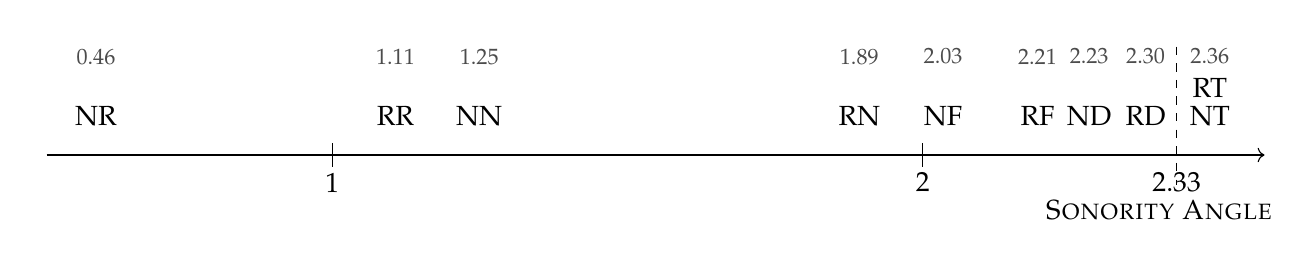
\begin{tikzpicture}[shorten >=1pt,->,scale=0.5]
     \tikzstyle{line} = [draw]%, -latex']

        \node (RT) at (2.48619449019234 * 15, 0.7) {RT};% 2.35619449019234 - repositioning for visual clarity
        \node (NT) at (2.48619449019234 * 15, 0) {NT}; % 2.35619449019234 - repositioning for visual clarity
        \node[font=\footnotesize,opacity=0.7] (NTno) at (2.48619449019234 * 15, 1.5) {2.36};
        \node (RD) at (2.37743866747662 * 15, 0) {RD}; % 2.29743866747662 
        \node[font=\footnotesize,opacity=0.7] (RDno) at (2.37743866747662 * 15, 1.5) {2.30};
        \node (ND) at (2.28183949564558 * 15, 0) {ND}; % 2.23183949564558 
        \node[font=\footnotesize,opacity=0.7] (NDno) at (2.28183949564558 * 15, 1.5) {2.23};
        \node (RF) at (2.19429743558818 * 15, 0) {RF}; % 2.21429743558818 
        \node[font=\footnotesize,opacity=0.7] (RFno) at (2.19429743558818 * 15, 1.5) {2.21};
        \node (NF) at (2.03444393579570 * 15, 0) {NF};
        \node[font=\footnotesize,opacity=0.7] (NFno) at (2.03444393579570 * 15, 1.5) {2.03};
        \node (RN) at (1.89254688119154 * 15, 0) {RN};
        \node[font=\footnotesize,opacity=0.7] (RNno) at (1.89254688119154 * 15, 1.5) {1.89};
        \node (NN) at (1.24904577239825 * 15, 0) {NN};
        \node[font=\footnotesize,opacity=0.7] (NNno) at (1.24904577239825 * 15, 1.5) {1.25};
        \node (RR) at (1.10714871779409 * 15, 0) {RR};
        \node[font=\footnotesize,opacity=0.7] (RRno) at (1.10714871779409 * 15, 1.5) {1.11};
        \node (NR) at (0.60 * 15, 0) {NR}; % 0.4636476090008
        \node[font=\footnotesize,opacity=0.7] (NRno) at (0.60 * 15, 1.5) {0.46};

    \node (axisstart) at (0.5 * 15,-1) {};
    \node (axisend)   at (2.6 * 15,-1) {};
    \draw (axisstart) -- (axisend);
   \node (xaxislabel) at (2.4 * 15,-2.4) {\textsc{Sonority Angle}};

  \node (dividinglinestart) at (2.43 * 15,2) {};
  \node (dividinglineend)   at (2.43 * 15,-2) {};
  \path [line,dashed] (dividinglinestart) -- (dividinglineend) -- cycle;

  \path [line] (2 * 15, -1.3) -- (2 * 15, -0.7) -- cycle;
  \path [line] (1 * 15, -1.3) -- (1 * 15, -0.7) -- cycle;
  \node (1mark) at (1 * 15, -1.7) {1};
  \node (2mark) at (2 * 15, -1.7) {2};

  \node (2pointlabel) at (2.43 * 15,-1.7) {2.33};
        

    \end{tikzpicture}

\bigskip

The sonorant-voiceless stop clusters can be neatly separated from the rest of the clusters in terms of {\sc Sonority Angle}.
The correct constraint ranking is therefore the following:

\ex. {\sc Ident(Son$\measuredangle$)$<$2.33} $\gg$ {\sc *Son-C} $\gg$ {\sc Ident(Son$\measuredangle$)$<$2.4}

\begin{center} \renewcommand*\arraystretch{1.2}
\scalebox{1}[1]{\begin{tabular}[t]{|rrl||c|c|c|} \hline 
\multicolumn{3}{|c||}{Input:~/\textipa{kork}/} & {\sc Ident(Son$\measuredangle$)$<$2.33} & {\sc *Son-C} & {\sc Ident(Son$\measuredangle$)$<$2.4} \\[0.5ex]
\hline \hline a. & \ding{43} & \textipa{kork} & & \cellcolor{lightgray}$\ast$ & \cellcolor{lightgray} \\
\hline b. & & \textipa{kor@k} & 2.36 $\ast$! & \cellcolor{lightgray} & \cellcolor{lightgray}2.36 $\ast$ \\
\hline \end{tabular}} \renewcommand*\arraystretch{1} \end{center}

\begin{center} \renewcommand*\arraystretch{1.2}
\scalebox{1}[1]{\begin{tabular}[t]{|rrl||c|c|c|} \hline 
\multicolumn{3}{|c||}{Input:~/\textipa{alb@}/} & {\sc Ident(Son$\measuredangle$)$<$2.33} & {\sc *Son-C} & {\sc Ident(Son$\measuredangle$)$<$2.4} \\[0.5ex]
\hline \hline c. & \ding{43} & \textipa{al@b@} & 2.29 & & \cellcolor{lightgray} 2.29 \\
\hline d. & & \textipa{alb@} & & $\ast$! & \cellcolor{lightgray} \\
\hline \end{tabular}} \renewcommand*\arraystretch{1} \end{center}

A note on the nasal-voiceless stop clusters is in order here: such clusters tend to be homorganic on the surface.  
It is therefore unclear whether such clusters failed to be broken up by epenthesis because of OCP, 
or because of the large sonority contour faithfulness violation.  
I argue that in general, it is for the second reason.

Suppose nasal-voiceless stop clusters were banned from epenthesising because of the OCP.
Then we would expect to see surface
sequences of [NVP] where N and P have different places of articulation and V is an epenthetic vowel, 
just as we see [NVB] sequences:

\ex. \a. [\textipa{b\textsuperscript{j}in\textsuperscript{j}ib}] \\
         {\it binb} `venom'
     \b. [\textipa{ban@b@}] \\
         {\it Banba} `Banba (a name for Ireland)'
     \z.
     \citep[2c]{carnie.1994}

To my knowledge, no [NVP] sequences with the properties stated above exist.

Further, albeit marginal, evidence comes from the existence of words with heterorganic [NP] sequences,
which are not broken up by epenthesis.

\ex. \a. [\textipa{s\textsuperscript{j}e:mt}] \\
         {\it s\'eimt} `the act of playing music', dialectal variant of {\it seinm})
     \b. [\textipa{k2r\textsuperscript{j}@m\textsuperscript{j}k\textsuperscript{j}}] \\
         {\it cuirimc} `I observe, pay attention to' (Connaught dialect) \\
     (Words found in \citet{dineen.2007})

I conclude that in general, epenthesis does not occur in /NT/ sequences due to the large {\sc Sonority Angle} between NT and NVT, and not to the non-existence of underlying heterorganic /NP/ clusters in the lexicon. The epenthetic facts of Irish thus support the ranking of NT and RT clusters at the bottom of the hierarchy of susceptibility to epenthesis, which is consistent with the {\sc Sonority Angle} metric.

\subsection{Comparison to other approaches}

An analysis based on {\sc Sonority Rise} \citep{flemming.2008} would be largely identical, but the cluster hierarchy would differ:

\ex. {\sc Sonority Rises}  of sonorant-initial clusters using revised sonority scale

 \begin{center}
  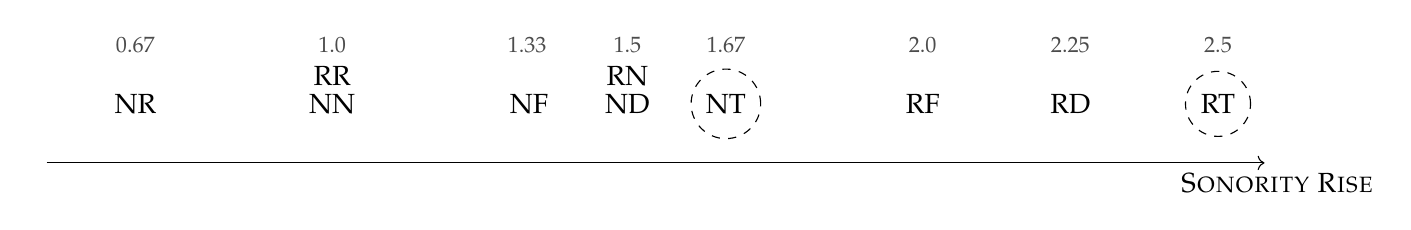
\begin{tikzpicture}[shorten >=1pt,->,scale=0.5]
     \tikzstyle{line} = [draw]%, -latex']

        \node[draw,circle,dashed] (NT) at (1.66666666666667 * 15, 0) {NT}; 
        \node[font=\footnotesize,opacity=0.7] (NTno) at (1.66666666666667  * 15, 1.5) {1.67};
        \node (ND) at (1.5 * 15, 0) {ND}; 
        \node[font=\footnotesize,opacity=0.7] (NDno) at (1.5 * 15, 1.5) {1.5};
        \node (NF) at (1.33333333333333 * 15, 0) {NF};
        \node[font=\footnotesize,opacity=0.7] (NDno) at (1.33 * 15, 1.5) {1.33};
        \node (NN) at (1 * 15, 0) {NN};
        \node[font=\footnotesize,opacity=0.7] (NDno) at (1 * 15, 1.5) {1.0};
        \node (NR) at (0.666666666666667 * 15, 0) {NR}; 
        \node[font=\footnotesize,opacity=0.7] (NDno) at (0.666666666666667* 15, 1.5) {0.67};

        \node[draw,circle,dashed] (RT) at (2.5 * 15, 0) {RT};
        \node[font=\footnotesize,opacity=0.7] (RTno) at (2.5 * 15, 1.5) {2.5};
        \node (RD) at (2.25 * 15, 0) {RD}; 
        \node[font=\footnotesize,opacity=0.7] (RDno) at (2.25 * 15, 1.5) {2.25};
        \node (RF) at (2 * 15, 0) {RF}; 
        \node[font=\footnotesize,opacity=0.7] (RFno) at (2 * 15, 1.5) {2.0};
        \node (RN) at (1.5 * 15, 0.7) {RN};
        \node (RR) at (1 * 15, 0.7) {RR};


    \node (axisstart) at (0.5 * 15,-1.5) {};
    \node (axisend)   at (2.6 * 15,-1.5) {};
    \draw (axisstart) -- (axisend);
   \node (xaxislabel) at (2.6 * 15,-2.0) {\textsc{Sonority Rise}};

    \end{tikzpicture} 
 \end{center}

Note that the clusters RF and RD fall between RT and NT on this scale.  Therefore, we cannot separate the clusters that undergo epenthesis from the ones that do not if we adopt {\sc Sonority Rise} as the relevant metric, as we can when we adopt {\sc Sonority Angle} (c.f. \ref{sonorantinitial_sonangle}).

\bigskip

%Carnie's (1994) analysis of these facts is in terms of a Minimal Distancing Constraint with various parameter settings, such as for which direction away from the nucleus it applies (to the right in the Irish case, to account for epenthesis applying to both codas and heterosyllabic clusters). His preliminary analysis has distance computed according to the following sonority scale:
%
%\ex. \label{carniesonorityscale} \a. 1 - Voiceless stops
%     \b. 2 - Voiced stops
%     \b. 3 - Voiceless fricatives
%     \b. 4 - Voiced fricatives
%     \b. 5 - Sonorants
%
%with a subsequent revision where sonority is computed in terms of the number of nodes that have to be specified to obtain the appropriate manner specification. This computation is somewhat complicated, so I will not reproduce it here. The result is that sonorant-fricative and sonorant-voiced stop clusters have a sonority distance of 0, since they are each specified for a single node in the feature geometry. Voiceless stops have no specified nodes, so sonorant-voiceless stop clusters have a sonority distance of 1, which is the minimal distance tolerated. 
%
%A sonority scale that gives nasals and liquids identical sonority values seems unlikely given measurable differences in the phonetic correlates of sonority such as intensity between liquids and nasals \citep{parker.2002}. This is especially so when the obstruents are spread so widely on the sonority scale. 
%I will therefore explore instead an alternative sonority distance-based analysis using Syllable Contact.


Now let us construct a markedness-based analysis for the Irish data.\footnote{\cite{carnie.1994} analyses these facts with a Minimal Distancing Constraint, based on a feature-geometric notion of sonority distance. The analysis presented here adheres more closely to the phonetic interpretation of sonority (see, for example, \cite{parker.2002}.}

Attempting to apply Syllable Contact to the Irish case, we immediately encounter problems. Firstly, it is difficult to see why markedness triggers epenthesis only in sonorant-initial clusters, as Syllable Contact predicts that obstruent-initial clusters should be even more marked.

Secondly, we would need to invoke a separate set of constraints on sonority sequencing in coda clusters, and assume that the ranking of the faithfulness constraint {\sc Dep} with respect to both sets of constraints is coincidentally identical.

Suppose then that we define a single markedness constraint that favours all falling sonority clusters regardless of their position in the syllable, i.e. combining Syllable Contact and Sonority Sequencing. We require a finer-grained metric to measure how marked a particular cluster is. An obvious course of action is to use \citet{gouskova.2002}'s {\sc Dis} metric, extending its use from the heterosyllabic environment alone to all positions. 

Using the defined sonority scale, we expect the following markedness hierarchy of sonorant-initial clusters.

\ex. {\sc Dis} values of sonorant-initial clusters using revised sonority scale

\begin{center}
  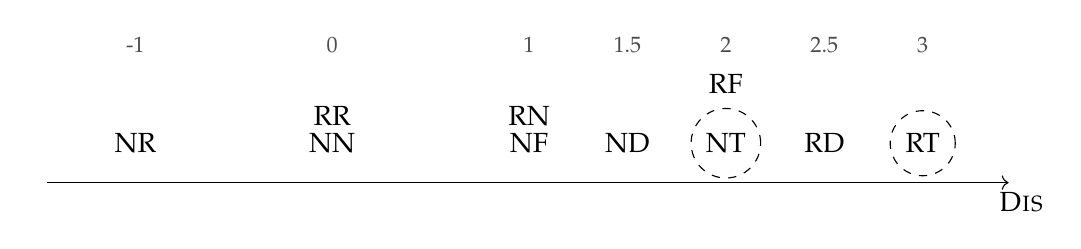
\begin{tikzpicture}[shorten >=1pt,->,scale=0.5]
     \tikzstyle{line} = [draw]%, -latex']

        \node[draw,circle,dashed] (NT) at (2 * 5, 0) {NT}; 
        \node[font=\footnotesize,opacity=0.7] (RTno) at (2 * 5, 2.5) {2};
        \node (ND) at (1.5 * 5, 0) {ND}; 
        \node[font=\footnotesize,opacity=0.7] (NDno) at (1.5 * 5, 2.5) {1.5};
        \node (NF) at (1 * 5, 0) {NF};
        \node[font=\footnotesize,opacity=0.7] (NFno) at (1 * 5, 2.5) {1};
        \node (NN) at (0 * 5, 0) {NN};
        \node[font=\footnotesize,opacity=0.7] (NNno) at (0 * 5, 2.5) {0};
        \node (NR) at (-1 * 5, 0) {NR}; 
        \node[font=\footnotesize,opacity=0.7] (NRno) at (-1 * 5, 2.5) {-1};

        \node[draw,circle,dashed] (RT) at (3 * 5, 0) {RT};
        \node[font=\footnotesize,opacity=0.7] (NDno) at (3 * 5, 2.5) {3};
        \node (RD) at (2.5 * 5, 0) {RD}; 
        \node[font=\footnotesize,opacity=0.7] (RDno) at (2.5 * 5, 2.5) {2.5};
        \node (RF) at (2 * 5, 1.5) {RF}; 
        \node (RN) at (1 * 5, 0.7) {RN};
        \node (RR) at (0 * 5, 0.7) {RR};

    \node (axisstart) at (-1.5 * 5,-1) {};
    \node (axisend)   at (3.5 * 5,-1) {};
    \draw (axisstart) -- (axisend);
  \node (xaxislabel) at (3.5 * 5,-1.5) {\textsc{Dis}};

    \end{tikzpicture} 
 \end{center}

Even ignoring the problem of the obstruent-initial clusters, we see that sonority distance
alone does not get us the desired result. Instead, it incorrectly predicts that if NT and RT are not 
broken up by epenthesis, then RF and RD should not either.

\subsection{Interim summary}

To summarise the findings of the Irish case study: a sonority contour faithfulness account explains
the facts quite simply, because {\sc Sonority Angle} successfully achieves a linear separation of
the NT and RT clusters from the remaining sonorant-initial clusters, explaining why they fail to undergo epenthesis. The {\sc Sonority Rise} metric does not have the same property. We have also seen that a markedness-based account would have to be much more complicated to explain the same facts.

\section{Case study: Chaha} \label{chaha}

Chaha is a Southern Semitic language spoken in central Ethiopia by about 440,000 people.  
As is common with Semitic languages, it has many underlying consonant clusters, some of which are resolved by epenthesis of the high central vowel [\textipa{1}].  Vowel epenthesis appears to preferentially target rising and level sonority clusters over falling ones.  The data in this section mostly comes from Rose 2000, who also provides an analysis in terms of Syllable Contact.

We will use the existing sonority scale given in \ref{standardsonorityscale}, with a small modification. Chaha has a bilabial approximant represented by [\textipa{B}] (more precisely, \textipa{\|`B}) \citep[15]{banksira.2000} that is not as sonorous as /r/, whose realisation is tap-like \citep[181]{taranto.2001}. The justification for /\textipa{B}/ being less sonorous than /r/ is largely empirical, based on the epenthetic behaviour of clusters containing this sonorant \citep[405]{rose.2000}, data for which will be presented later in this paper. I will specify its sonority as an intermediate 3.5, under the sonority of 4 for liquids in general.

\ex. Sonority scale to be used in Chaha

\vspace{-1.5em}
\begin{center}
\begin{tabular}{ccccccccccccc}
 V & $>$ & w j & $>$ & r & $>$ & \textipa{B} & $>$ & m n & $>$ & f s z x & $>$ & t t' k k' d g \\
 vowels & & glides & & liquids & &   & & nasals & & fricatives & & stops \\
    V   & &    G   & &    R    & & \textipa{B} & & N & & F & & T \\
    6   & &    5   & &    4    & &    3.5      & & 3 & & 2 & & 1 \\
\end{tabular}
\end{center}

\subsection{CC clusters}

\subsubsection{Data}

Underlying two-consonant clusters in Chaha are obligatorily epenthesised into if initial, never broken up by epenthesis in medial position, while final clusters are epenthesised into if they are of rising or level sonority, or the cluster consists of [r] followed by a nasal.

\ex. No onset clusters in Chaha
     \a. \textipa{k1r@tam} `he lifted up' \citep[398]{rose.2000}
     
\ex. Tautomorphemic medial two-consonant clusters are tolerated no matter what their sonority profile
     \a. \textipa{s1rto} `cauterise ({\sc masc pl})!'
     \b. \textipa{n1k'mo} `pick ({\sc masc pl})!'
     \b. \textipa{at'met'} `solidified juice from [\textipa{@s@t}] plant'
     \z. \citep[(1a,c,d)]{rose.2000}

The presentation of the patterns of epenthesis in CC\# clusters is slightly complicated by variability between idiolects.  Epenthesis is possible in all level and rising sonority clusters.  
Among these clusters, the ones for which epenthesis is optionally unavailable are the obstruent-obstruent clusters.  Most falling sonority clusters do not undergo epenthesis,
except [r]-sonorant clusters, which can be broken up in certain idiolects. Voicing is irrelevant
to whether clusters undergo epenthesis.

The following table summarises the data.

\ex. Table showing epenthesis patterns for clusters of varying sonority patterns:

\begin{tabular}{c | c c c c c}
 \backslashbox{C\textsubscript{1}}{C\textsubscript{2}}      & Stop & Fricative & Nasal & Liquid \\ \hline
Stop   & \textbf{OPTIONAL}   & \textbf{OPTIONAL} & \textbf{\tickYes} & \textbf{\tickYes} \\
       & \textipa{n1g(1)d} & \textipa{d1g(1)s} & \textipa{n1k1m} & \textipa{g1d1r} \\
       & `touch!' & `give feast!' & `pick!' & `put to bed!' \\ \hline
Fric-  & \textbf{\tickNo} & \textbf{OPTIONAL} & \textbf{\tickYes} & \textbf{\tickYes} \\
ative  & \textipa{k1ft}   & \textipa{mes(1)x} &    & \textipa{s1f1r} \\
       & `open!'  & `chew!' & & `measure!' & \\ \hline
Nasal  & \textbf{\tickNo}     & \textbf{\tickNo}     & \textbf{\tickYes} & \textbf{\tickYes} \\
       & \textipa{g1nd} & \textipa{t1mx} & \textipa{g@n1m}   &  \\
       & `log (noun)'   & `scoop with finger!' & `take back loaned cow!' &  \\ \hline
Liquid & \textbf{\tickNo}     & \textbf{\tickNo} & \textbf{OPTIONAL}      & \textbf{\tickYes} \\
       & \textipa{f1rt} & \textipa{t1rx} & \textipa{k1r(1)m} & \textipa{s1B1r} \\
       & `divide in half!' & `make incision!' & `insult!'    & `break!' \\  \hline
\end{tabular}	
\noindent (Data assembled from \citet[404--7]{rose.2000})

\bigskip

The variability therefore lies in (1) whether epenthesis between obstruents is possible (between stops, between a stop and a fricative, and between two fricatives), and (2) whether [r]-sonorant can be broken up by epenthesis or not.

The variable setting of these two options corresponds to four attested idiolects:

  \ex. \label{idiolects} The four idiolects: \citep[(43)]{rose.2000}
       \a. \label{idiolecta} \tickYes OVO, \tickNo rVN \citep{leslau.1964} \newline % \textsc{SonSeq} $\gg$ \textsc{SyllCon} $\gg$ \textsc{Dep-IO} $\gg$ \textsc{*R-Son} \newline
           [\textipa{k1rm}], [\textipa{s1B1r}], [\textipa{k1ft}], [\textipa{k1t1f}], [\textipa{s1g1d}]
       \b. \label{idiolectb} \tickYes OVO, \tickYes rVN \newline %\label{idiolectc} \textsc{SonSeq, *R-Son} $\gg$ \textsc{SyllCon} $\gg$ \textsc{Dep-IO} \newline
           [\textipa{k1r1m}], [\textipa{s1B1r}], [\textipa{k1ft}], [\textipa{k1t1f}], [\textipa{s1g1d}]
       \c. \label{idiolectc} \tickNo OVO, \tickNo rVN \newline %\label{idiolectb} \textsc{SyllCon} $\gg$ \textsc{Dep-IO} $\gg$ \textsc{SonSeq, *R-Son} \newline
           [\textipa{k1rm}], [\textipa{s1B1r}], [\textipa{k1ft}], [\textipa{k1tf}], [\textipa{s1gd}]
       \d. \label{idiolectd} \tickNo OVO, \tickYes rVN \newline %\label{idiolectd} \textsc{*R-Son} $\gg$ \textsc{SyllCon} $\gg$ \textsc{Dep-IO} $\gg$ \textsc{SonSeq} \newline
           [\textipa{k1r1m}], [\textipa{s1B1r}], [\textipa{k1ft}], [\textipa{k1tf}], [\textipa{s1gd}]


\subsubsection{Analysis}

Under a sonority contour faithfulness analysis, epenthesis is triggered by a markedness constraint on the structural conditions of the cluster, not by the markedness of the underlying sonority contour profile itself. Undominated {\sc *ComplexOnset} accounts for the non-existence of initial clusters. {\sc *Coda} is ranked low, and therefore medial clusters are left intact.{\sc *ComplexCoda}, dominated by an {\sc Ident(Son$\measuredangle$)} constraint, explains why some coda clusters are broken up by epenthesis while others are not.

In idiolect \ref{idiolecta}, all coda clusters of rising and level sonority -- that is, those with a {\sc Sonority Angle} smaller than 1.5 -- are broken up by epenthesis, while falling sonority clusters -- those with a {\sc Sonority Angle} greater than 1.5 -- are left intact. 

\ex. All clusters with a {\sc Sonority Angle} to the left of the dividing line undergo epenthesis while those to the right resist it, with one exception.

\resizebox{\linewidth}{!}{
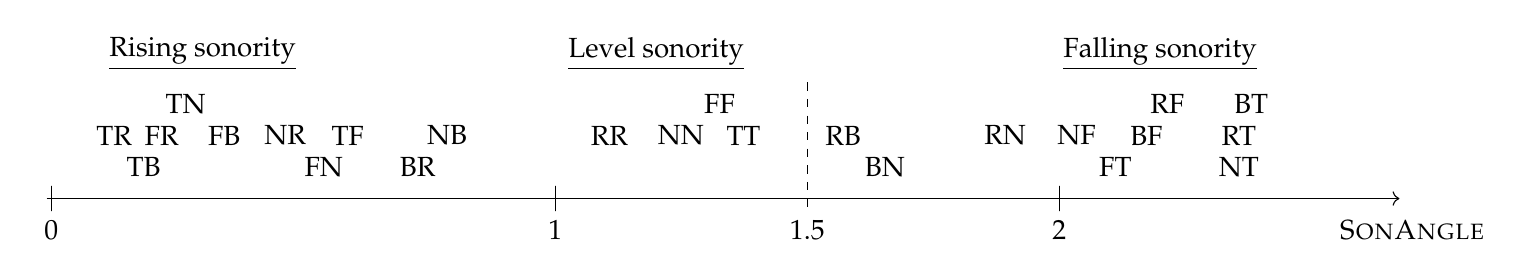
\begin{tikzpicture}[scale=0.8,shorten >=1pt,->]
  \tikzstyle{point}=[circle,fill=black!25,minimum size=12pt,inner sep=2pt]
  \tikzstyle{line} = [draw, -latex']

	\node (TR) at (0.124354994547*8, 1) {TR};
	\node (Tb) at (0.183110817262*8, 0.5) {T\textipa{B}};
	\node (FR) at (0.218668945874*8, 1) {FR};
	\node (TN) at (0.266252049151*8, 1.5) {TN};
	\node (Fb) at (0.343023940421*8, 1) {F\textipa{B}};
	\node (NR) at (0.463647609001*8, 1) {NR};
	\node (FN) at (0.540419500271*8, 0.5) {FN};
	\node (TF) at (0.588002603548*8, 1) {TF};
	\node (bR) at (0.726642340682*8, 0.5) {\textipa{B}R};
	\node (Nb) at (0.785398163397*8, 1) {N\textipa{B}};
	\node (RR) at (1.10714871779*8, 1) {RR};
%	\node (bb) at (1.19028994968*8, 0.5) {\textipa{BB}};
	\node (NN) at (1.2490457724*8, 1) {NN};
	\node (FF) at (1.32581766367*8, 1.5) {FF};
	\node (TT) at (1.37340076695*8, 1) {TT};
	\node (Rb) at (1.57079632679*8, 1) {R\textipa{B}};
	\node (bN) at (1.65393755868*8, 0.5) {\textipa{B}N};
	\node (RN) at (1.89254688119*8, 1) {RN};
	\node (NF) at (2.0344439358*8, 1) {NF};
%	\node (GF) at (2.0344439358*8, 1.5) {GF};
	\node (FT) at (2.11121582707*8, 0.5) {FT};
	\node (bF) at (2.17308367293*8, 1) {\textipa{B}F};
	\node (RF) at (2.21429743559*8, 1.5) {RF};
	\node (RT) at (2.35619449019*8, 1) {RT};
	\node (NT) at (2.35619449019*8, 0.5) {NT};
	\node (bT) at (2.38057989937*8, 1.5) {\textipa{B}T};
  \node (rising) at (0.3*8,2.3) {\underline{Rising sonority}};
  \node (level) at (1.2*8,2.3) {\underline{Level sonority}};
  \node (falling) at (2.2*8,2.3) {\underline{Falling sonority}};
  % axis
  \node (axisstart) at (-0.23,0) {};
  \node (axisend)   at (2.7*8,0) {};
  \draw (axisstart) -- (axisend);
  \draw (0.0*8, 0.2) -- (0.0*8, -0.2) -- cycle;
  \draw (1.0*8, 0.2) -- (1.0*8, -0.2) -- cycle;
  \draw (2.0*8, 0.2) -- (2.0*8, -0.2) -- cycle;
  \node (0pointlabel) at (0.0,-0.5) {0};
  \node (1pointlabel) at (1.0*8,-0.5) {1};
  \node (2pointlabel) at (2.0*8,-0.5) {2};
  \node (xaxislabel) at (2.7*8,-0.5) {\textsc{SonAngle}};
  % dividing line
  \node (dividinglinestart) at (1.5 * 8,2) {};
  \node (dividinglineend)   at (1.5 * 8,-0.3) {};
  \path [line,dashed] (dividinglinestart) -- (dividinglineend) -- cycle;
  \node (dividingpointlabel) at (1.5*8, -0.5) {1.5};
\end{tikzpicture}
}

The constraint ranking for this idiolect is thus:

\ex. {\sc Ident(Son$\measuredangle$)}$<$1.5 $\gg$ {\sc *ComplexCoda}

\begin{center} \renewcommand*\arraystretch{1.2}
\scalebox{1}[1]{\begin{tabular}[t]{|rrl||c|c|} \hline 
\multicolumn{3}{|c||}{Input:~/\textipa{k1tf}/} & {\sc Ident(Son$\measuredangle$)}$<$1.5 & {\sc *ComplexCoda} \\[0.5ex]
\hline \hline a. & & \textipa{k1tf} & & $\ast$! \\
\hline b. & \ding{43} & \textipa{k1t1f} & 0.59 & \\
\hline \end{tabular}} \renewcommand*\arraystretch{1} \end{center}

\begin{center} \renewcommand*\arraystretch{1.2}
\scalebox{1}[1]{\begin{tabular}[t]{|rrl||c|c|} \hline 
\multicolumn{3}{|c||}{Input:~/\textipa{k1rm}/} & {\sc Ident(Son$\measuredangle$)}$<$1.5 & {\sc *ComplexCoda} \\[0.5ex]
\hline \hline c. &  \ding{43} & \textipa{k1rm} & & $\ast$ \\
\hline d. & & \textipa{k1r1m} & 1.89 $\ast$! & \\
\hline \end{tabular}} \renewcommand*\arraystretch{1} \end{center}

This approach does make one incorrect prediction: it predicts that /\textipa{Bm}/ should not undergo epenthesis under this ranking, since /\textipa{B}N/ has a {\sc Sonority Angle} of 1.65. But it always does:

\ex. /\textipa{s@B-m}/ $\rightarrow$ \textipa{s@B1m} `people-{\sc emph}'  \citep[fn. 16]{rose.2000}

The only clusters that give us evidence of this are /\textipa{Bm}/ clusters. These are not seen root-internally due to a high-ranking OCP effect \citep[cited in \cite{rose.2000}]{greenberg.1950}.
I suggest that there might be an undominated markedness constraint against this cluster -- either OCP(labial) or another constraint based on articulatory or perceptual difficulty -- that outranks all relevant faithfulness constraints.

\bigskip

Proceeding to idiolect \ref{idiolectb}, we find that [r]-sonorant clusters are allowed to undergo epenthesis word-finally. Because {\sc Sonority Angle} permits a linear separation of the [r]-sonorant clusters from the remainder of the falling sonority clusters, this is straightforward to explain
by the movement of the cut-off line from 1.5 to 1.9.

\bigskip
\resizebox{\linewidth}{!}{
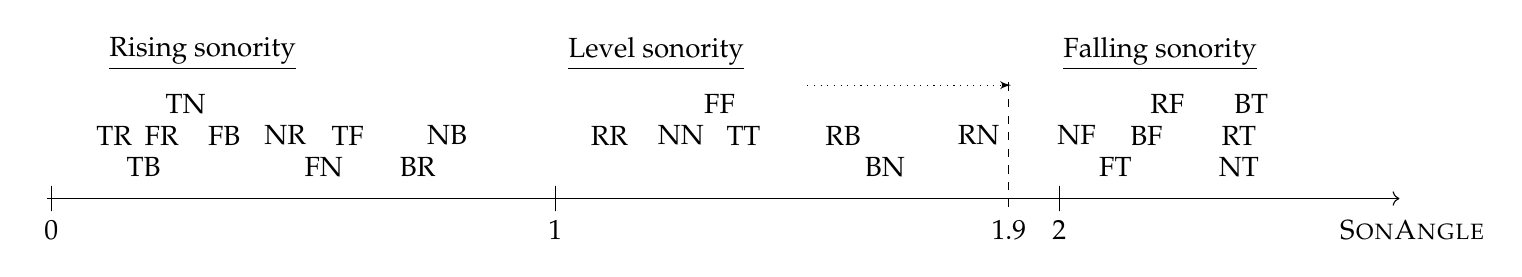
\begin{tikzpicture}[scale=0.8,shorten >=1pt,->]
  \tikzstyle{point}=[circle,fill=black!25,minimum size=12pt,inner sep=2pt]
  \tikzstyle{line} = [draw, -latex']

	\node (TR) at (0.124354994547*8, 1) {TR};
	\node (Tb) at (0.183110817262*8, 0.5) {T\textipa{B}};
	\node (FR) at (0.218668945874*8, 1) {FR};
	\node (TN) at (0.266252049151*8, 1.5) {TN};
	\node (Fb) at (0.343023940421*8, 1) {F\textipa{B}};
	\node (NR) at (0.463647609001*8, 1) {NR};
	\node (FN) at (0.540419500271*8, 0.5) {FN};
	\node (TF) at (0.588002603548*8, 1) {TF};
	\node (bR) at (0.726642340682*8, 0.5) {\textipa{B}R};
	\node (Nb) at (0.785398163397*8, 1) {N\textipa{B}};
	\node (RR) at (1.10714871779*8, 1) {RR};
%	\node (bb) at (1.19028994968*8, 0.5) {\textipa{BB}};
	\node (NN) at (1.2490457724*8, 1) {NN};
	\node (FF) at (1.32581766367*8, 1.5) {FF};
	\node (TT) at (1.37340076695*8, 1) {TT};
	\node (Rb) at (1.57079632679*8, 1) {R\textipa{B}};
	\node (bN) at (1.65393755868*8, 0.5) {\textipa{B}N};
	\node (RN) at (1.84*8, 1) {RN}; %1.89254688119
	\node (NF) at (2.0344439358*8, 1) {NF};
%	\node (GF) at (2.0344439358*8, 1.5) {GF};
	\node (FT) at (2.11121582707*8, 0.5) {FT};
	\node (bF) at (2.17308367293*8, 1) {\textipa{B}F};
	\node (RF) at (2.21429743559*8, 1.5) {RF};
	\node (RT) at (2.35619449019*8, 1) {RT};
	\node (NT) at (2.35619449019*8, 0.5) {NT};
	\node (bT) at (2.38057989937*8, 1.5) {\textipa{B}T};
  \node (rising) at (0.3*8,2.3) {\underline{Rising sonority}};
  \node (level) at (1.2*8,2.3) {\underline{Level sonority}};
  \node (falling) at (2.2*8,2.3) {\underline{Falling sonority}};
  % axis
  \node (axisstart) at (-0.23,0) {};
  \node (axisend)   at (2.7*8,0) {};
  \draw (axisstart) -- (axisend);
  \draw (0.0*8, 0.2) -- (0.0*8, -0.2) -- cycle;
  \draw (1.0*8, 0.2) -- (1.0*8, -0.2) -- cycle;
  \draw (2.0*8, 0.2) -- (2.0*8, -0.2) -- cycle;
  \node (0pointlabel) at (0.0,-0.5) {0};
  \node (1pointlabel) at (1.0*8,-0.5) {1};
  \node (2pointlabel) at (2.0*8,-0.5) {2};
  \node (xaxislabel) at (2.7*8,-0.5) {\textsc{SonAngle}};
  % dividing line
  \node (dividinglinestart) at (1.9 * 8,2) {};
  \node (dividinglineend)   at (1.9 * 8,-0.3) {};
  \path [line,dashed] (dividinglinestart) -- (dividinglineend) -- cycle;
  \node (dividingpointlabel) at (1.9*8, -0.5) {1.9};
  \path [line,dotted] (1.5 * 8,1.8) -- (1.91 * 8, 1.8);
\end{tikzpicture}
}

\ex. {\sc Ident(Son$\measuredangle$)}$<$1.9 $\gg$ {\sc *ComplexCoda}

\begin{center} \renewcommand*\arraystretch{1.2}
\scalebox{1}[1]{\begin{tabular}[t]{|rrl||c|c|} \hline 
\multicolumn{3}{|c||}{Input:~/\textipa{k1rm}/} & {\sc Ident(Son$\measuredangle$)}$<$1.9 & {\sc *ComplexCoda} \\[0.5ex]
\hline \hline a. &   & \textipa{k1rm} & & $\ast$! \\
\hline b. & \ding{43} & \textipa{k1r1m} & 1.89 & \\
\hline \end{tabular}} \renewcommand*\arraystretch{1} \end{center}

Idiolects \ref{idiolectc} and \ref{idiolectd} are identical to \ref{idiolecta} and \ref{idiolectb} respectively, except that obstruent-obstruent clusters do not undergo epenthesis under any circumstances. This can be achieved by ranking {\sc Dep}(+son)
above {\sc *ComplexCoda}.

\ex. Ranking for idiolect \ref{idiolectc}

\begin{center} \renewcommand*\arraystretch{1.2}
\scalebox{1}[1]{\begin{tabular}[t]{|rrl||c:c|c|} \hline 
\multicolumn{3}{|c||}{Input:~/\textipa{s1gd}/} & {\sc Dep}(+son) & {\sc Ident(Son$\measuredangle$)}$<$1.5 & {\sc *ComplexCoda} \\[0.5ex]
\hline \hline a. & \ding{43} & \textipa{s1gd} & & & \cellcolor{lightgray}$\ast$ \\
\hline b. & & \textipa{s1g1d} & $\ast$! & 1.37 & \cellcolor{lightgray} \\
\hline \end{tabular}} \renewcommand*\arraystretch{1} \end{center}

To summarise, coda epenthesis behaviour in Chaha can be explained by the ranking of a {\sc Ident(Son$\measuredangle$)}$<$n constraint above the markedness constraint triggering epenthesis, {\sc *ComplexCoda}. The evidence of the epenthetic behaviour of Chaha coda clusters accords with the {\sc Sonority Angle} prediction that RN should be the most likely to epenthesise out of the falling sonority clusters. It also demonstrates the action of a faithfulness constraint against introducing a sonorant region between two obstruents, {\sc Dep}(+son), as defined in $\S$\ref{depson}.

\ex. Rankings for the four idiolects:
     \a. {\sc Ident(Son$\measuredangle$)}$<$1.5 $\gg$ {\sc *ComplexCoda} $\gg$ {\sc Dep}(+son)
     \b. {\sc Ident(Son$\measuredangle$)}$<$1.9 $\gg$ {\sc *ComplexCoda} $\gg$ {\sc Dep}(+son)
     \c. {\sc Ident(Son$\measuredangle$)}$<$1.5, {\sc Dep}(+son) $\gg$ {\sc *ComplexCoda}
     \c. {\sc Ident(Son$\measuredangle$)}$<$1.9, {\sc Dep}(+son) $\gg$ {\sc *ComplexCoda}

\subsubsection{Comparison to other approaches}

{\sc Sonority Rise} \citep{flemming.2008} can explain idiolects \ref{idiolecta} and \ref{idiolectc}, where the cut-off is drawn between rising and level sonority clusters on the one hand and falling sonority clusters on the other. It is less straightforward to explain the behaviour of idiolects \ref{idiolectb} and \ref{idiolectd}. This is because the cluster hierarchy predicted by {\sc Sonority Rise} does not permit a linear separation of [r]-sonorant clusters from the other falling sonority clusters: if RN undergoes epenthesis, we expect that FT and NF should also do so, but FT never does.

\ex. No linear separation between the rising and level sonority clusters plus RN from the rest of the falling sonority clusters under the {\sc Sonority Rise} metric.

\resizebox{\linewidth}{!}{
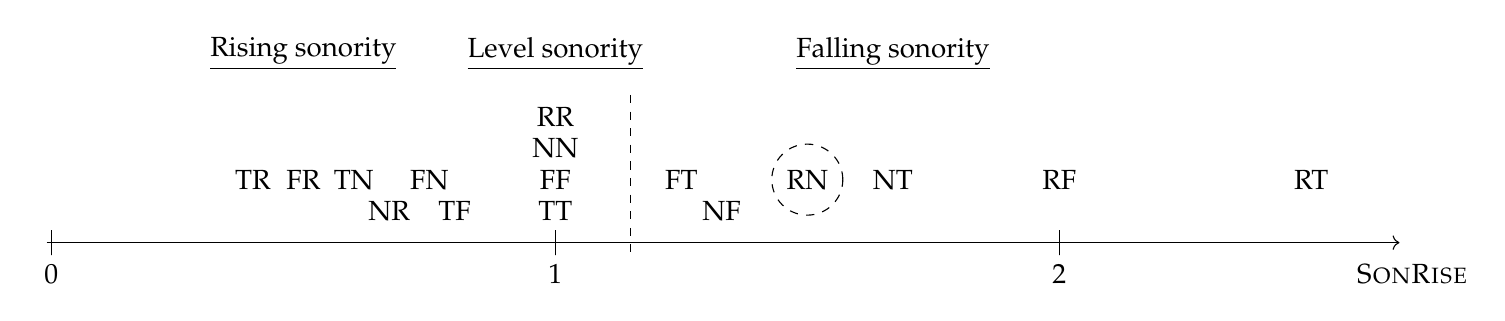
\begin{tikzpicture}[scale=0.8,shorten >=1pt,->]
  \tikzstyle{line} = [draw, -latex']
  \node (RT) at (2.5*8, 0)  {RT};
  \node (NT) at (1.67*8,0)  {NT};
  \node (FT) at (1.25*8,0)  {FT};
  \node (TT) at (1*8,-0.5)     {TT};
  \node (RF) at (2*8,0)     {RF};
  \node (NF) at (1.33*8,-0.5)  {NF};
  \node (FF) at (1*8,0)   {FF};
  \node (TF) at (0.8*8,-0.5)   {TF};
  \node[draw,circle,dashed] (RN) at (1.5*8,0)   {RN};
  \node (NN) at (1*8,0.5)     {NN};
  \node (FN) at (0.75*8,0)  {FN};
  \node (TN) at (0.6*8,0)   {TN};
  \node (RR) at (1*8,1.0)  {RR};
  \node (NR) at (0.67*8,-0.5)  {NR};
  \node (FR) at (0.5*8,0)   {FR};
  \node (TR) at (0.4*8,0)   {TR};
  \node (rising) at (0.5*8,2) {\underline{Rising sonority}};
  \node (level) at (1*8,2) {\underline{Level sonority}};
  \node (falling) at (1.67*8,2) {\underline{Falling sonority}};
  % axis
  \node (axisstart) at (-0.23,-1.0) {};
  \node (axisend)   at (2.7*8,-1.0) {};
  \draw (axisstart) -- (axisend);
  \draw (0.0*8, -1.2) -- (0.0*8, -0.8) -- cycle;
  \draw (1.0*8, -1.2) -- (1.0*8, -0.8) -- cycle;
  \draw (2.0*8, -1.2) -- (2.0*8, -0.8) -- cycle;
  \node (0pointlabel) at (0.0,-1.5) {0};
  \node (1pointlabel) at (1.0*8,-1.5) {1};
  \node (2pointlabel) at (2.0*8,-1.5) {2};
  \node (xaxislabel) at (2.7*8,-1.5) {\textsc{SonRise}};
  % dividing line
  \node (dividinglinestart) at (1.15 * 8,1.5) {};
  \node (dividinglineend)   at (1.15 * 8,-1.3) {};
  \path [line,dashed] (dividinglinestart) -- (dividinglineend) -- cycle;
\end{tikzpicture}
}

\bigskip

\citet{rose.2000} offers an explanation for these facts in terms of markedness of the sonority contours of the surface clusters. Medial clusters are subject to Syllable Contact, which bans rising sonority clusters across a syllable boundary, while coda clusters are subject to Sonority Sequencing.

The fact that medial clusters are never broken up by epenthesis even when they violate Syllable Contact is due to a constraint against the configuration [V.C\textipa{1}.CV], {\sc *MedialLight}. This constraint is unnecessary under my analysis as the only constraint that would militate against medial clusters, {\sc *Coda}, is not active.

In addition, Sonority Sequencing does not allow a divide of the [r]-sonorant clusters versus the remainder of the clusters, whether in Rose's categorical formulation of Sonority Sequencing or a family of {\sc *Dis} constraints.

\newpage

\ex. No linear separation between the rising and level sonority clusters plus RN from the rest of the falling sonority clusters under the {\sc Dis} metric.

\resizebox{\linewidth}{!}{
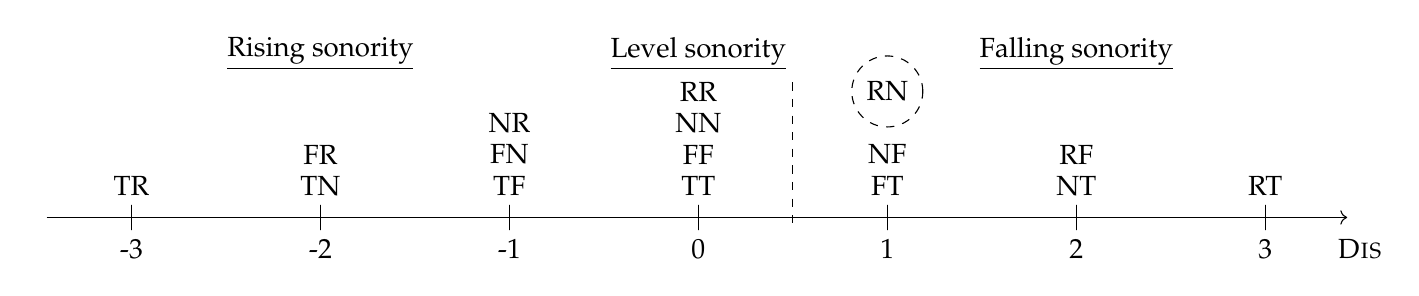
\begin{tikzpicture}[scale=0.8,shorten >=1pt,->]
  \tikzstyle{vertex}=[circle]
  \tikzstyle{point}=[circle,fill=black!25,minimum size=12pt,inner sep=2pt]
  \tikzstyle{line} = [draw, -latex']
  \node (RT) at (3*3,0.5)   {RT};
  \node (NT) at (2*3,0.5)  {NT};
  \node (FT) at (1*3,0.5)  {FT};
  \node (TT) at (0*3,0.5)     {TT};
  \node (RF) at (2*3,1.0)     {RF};
  \node (NF) at (1*3,1.0)  {NF};
  \node (FF) at (0*3,1.0)   {FF};
  \node (TF) at (-1*3,0.5)   {TF};
  \node[circle,draw,dashed] (RN) at (1*3,2.0)   {RN};
  \node (NN) at (0*3,1.5)   {NN};
  \node (FN) at (-1*3,1)  {FN};
  \node (TN) at (-2*3,0.5)   {TN};
  \node (RR) at (0*3,2.0)  {RR};
  \node (NR) at (-1*3,1.5)  {NR};
  \node (FR) at (-2*3,1.0)   {FR};
  \node (TR) at (-3*3,0.5)   {TR};
  % headers
  \node (rising) at (2*3,2.6) {\underline{Falling sonority}};
  \node (level) at (0*3,2.6) {\underline{Level sonority}};
  \node (falling) at (-2*3,2.6) {\underline{Rising sonority}};
  % axis
  \node (axisstart) at (-3.5*3,-0) {};
  \node (axisend)   at (3.5*3,-0) {};
  \draw (axisstart) -- (axisend);
  \draw (0, 0.2) -- (0, -0.2) -- cycle;
  \draw (1*3, 0.2) -- (1*3, -0.2) -- cycle;
  \draw (2*3, 0.2) -- (2*3, -0.2) -- cycle;
  \draw (3*3, 0.2) -- (3*3, -0.2) -- cycle;
  \draw (-1*3, 0.2) -- (-1*3, -0.2) -- cycle;
  \draw (-2*3, 0.2) -- (-2*3, -0.2) -- cycle;
  \draw (-3*3, 0.2) -- (-3*3, -0.2) -- cycle;
  \node (0pointlabel) at (0.0,-0.5) {0};
  \node (1pointlabel) at (1.0*3,-0.5) {1};
  \node (2pointlabel) at (2.0*3,-0.5) {2};
  \node (3pointlabel) at (3.0*3,-0.5) {3};
  \node (-1pointlabel) at (-1.0*3,-0.5) {-1};
  \node (-2pointlabel) at (-2.0*3,-0.5) {-2};
  \node (-3pointlabel) at (-3.0*3,-0.5) {-3};
  \node (xaxislabel) at (3.5*3,-0.5) {\textsc{Dis}};
  % dividing line
  \node (dividinglinestart) at (0.5 * 3,2.3) {};
  \node (dividinglineend)   at (0.5 * 3,-0.3) {};
  \path [line,dashed] (dividinglinestart) -- (dividinglineend) -- cycle;
\end{tikzpicture}
}

Therefore, Rose needs to invoke the following constraint to cause epenthesis in these clusters:

\ex. {\sc *R-Sonorant}: no [r]-sonorant sequences \citep[(41)]{rose.2000}

For those speakers that permit obstruent-obstruent clusters in defiance of Sonority Sequencing, Rose ranks Sonority Sequencing low, using the following constraint to trigger epenthesis in other clusters instead:

\ex. {\sc *C-Son\#}: a word-final sonorant consonant must be preceded by a vowel or [r].

Rose's approach thus requires the formulation of two constraints specifically targeting [r]. The advantage of doing so is that it avoids the difficulty of forbidding [\textipa{Bm}] clusters which we encountered above. On the other hand, the sonority contour faithfulness approach does not have to single out [r] for special treatment at all, by virtue of the ability of the {\sc Sonority Angle} hierarchy to group [r]-sonorant clusters together with the level and rising sonority clusters, at the expense of requiring a constraint against [\textipa{Bm}] clusters.

\subsection{CCC clusters}

Triconsonantal clusters are always broken up as [CC\textipa{1}C] or [C\textipa{1}CC]. The sources of CCC clusters in Chaha are the 3rd singular masculine conjugation of the jussive form of triliteral verbs, which have the underlying form /j\textipa{@}-\underline{CCC}-o/, and
the 3rd singular masculine conjugation of the passive/reflexive form of quadriliteral verbs,
which have the underlying form /j-\underline{t-CC}aCaC/.

As with coda clusters, there is considerable inter- and intra-speaker variability in epenthetic positioning.

\subsubsection{Data and Analysis} \label{CCCanalysis}

Triconsonantal clusters must be broken up via epenthesis, indicating that {\sc *CCC} $\gg$ {\sc Dep}. If epenthesis occurs either between C\textsubscript{1}C\textsubscript{2} or between C\textsubscript{2}C\textsubscript{3}, {\sc *CCC} will be satisfied. We do not need a separate constraint to prevent double epenthesis occurring to produce *[C\textipa{1}C\textipa{1}C]. 

\newpage
\ex. {\sc *CCC} $\gg$ {\sc Dep}

\vspace{-2em}
\begin{center} \renewcommand*\arraystretch{1.2}
\scalebox{1}[1]{\begin{tabular}[t]{|rrl||c|c|} \hline 
\multicolumn{3}{|c||}{Input:~/CCC/} & *CCC & {\sc Dep} \\[0.5ex]
\hline \hline a. & & CCC & $\ast$! &  \\
\hline b. & \ding{43} & CC\textipa{1}C & & $\ast$ \\
\hline c. & \ding{43} & C\textipa{1}CC & & $\ast$ \\
\hline d. & & C\textipa{1}C\textipa{1}C & & $\ast\ast$! \\
\hline \end{tabular}} \renewcommand*\arraystretch{1} \end{center}

This holds for all the ``idiolects'' reported in \citep{rose.2000}. Within each, we need only explain the location of epenthesis.

There are four idiolects to be explained. Note that these do not appear to correlate systematically with the four coda cluster idiolects.

\ex. \a. ``Default idiolect'', discussed in Section 4.3 of \citep{rose.2000}. \label{defaultCCCidiolect}
           \a. [C\textipa{1}CC] iff C\textsubscript{1}C\textsubscript{2} is a rise or plateau and C\textsubscript{2}C\textsubscript{3} is a fall.
           \b. [CC\textipa{1}C] otherwise.
           \z.
     \b. [CR\textipa{1}N] idiolect, discussed in Section 5.2.2 of \citep{rose.2000}. \label{CRNidiolect}
           \a. [CC\textipa{1}C] if C\textsubscript{2} is [r] and C\textsubscript{3} is a sonorant.
           \b. Otherwise as default.
           \z.
     \c. [C\textipa{1}CC] idiolect, discussed in Section 5.2.1 of \citep{rose.2000}. \label{C1CCidiolect}
           \a. [CC\textipa{1}C] iff C\textsubscript{2}C\textsubscript{3} is a fall and C\textsubscript{1}C\textsubscript{2} is a rise or plateau.
           \b. [C\textipa{1}CC] otherwise.
           \z.
     \d. [\textipa{w1zf}, \textipa{s1gd}] idiolect, discussed in Section 5.2.1 of \citep{rose.2000}. \label{wizfidiolect}
          \a. In this idiolect alone, /wzf/ and /sgd/ epenthesise as [\textipa{w1zf}] and  [\textipa{s1gd}].

\bigskip

\noindent {\bf Default idiolect.} In the default idiolect \ref{defaultCCCidiolect}, epenthesis occurs between C\textsubscript{2} and C\textsubscript{3} to form [CC\textipa{1}C].
Only when C\textsubscript{1}C\textsubscript{2} constitutes a sonority rise or plateau, and C\textsubscript{2}C\textsubscript{3} constitutes a sonority fall, does epenthesis occur between C\textsubscript{1} and C\textsubscript{2} to form [C\textipa{1}CC]. Forms and their associated sonority angles are shown in the table below. Underlined forms have alternate forms in other idiolects.

\ex. Default idiolect \citep[(24,26,28,30,32)]{rose.2000} \label{defaultidiolectCCCforms}

\begin{longtable}{ccccc}
	& Underlying form      & Surface form & {\sc SonAngle}(C\textsubscript{1},C\textsubscript{2}) & {\sc SonAngle}(C\textsubscript{2},C\textsubscript{3}) \\ \hline
    \multicolumn{5}{c}{Fall-\{Rise, Plateau\}: [CC\textipa{1}C]} \\ \hline
	a. & \textipa{j@-rk't'-o} & \textipa{j@nk'1t'o} & 2.36 & 1.37 \\
	b. & \textipa{j@-rks-o}   & \textipa{j@nk1so}   & 2.36 & 0.59 \\
    c. & \textipa{j@-rk'm-o}  & \textipa{j@nk'1mo}  & 2.36 & 0.27 \\
    d. & \textipa{j@-\underline{wzf}-o} & \textipa{j@wz1fo} & 2.03 & 1.33 \\
	e. & \textipa{j@-mxr-o}   & \textipa{j@mx1ro}   & 2.03 & 0.22 \\
    f. & \textipa{j@-\underline{sgd}-o} & \textipa{j@sg1do}   & 2.11 & 1.37 \\  
    g. & \textipa{j@-sdB-o}   & \textipa{j@sd1Bo}   & 2.11 & 0.18 \\ \hline 
    \multicolumn{5}{c}{\{Rise, Plateau\}-\{Rise, Plateau\}: [CC\textipa{1}C]} \\ \hline
    h. & \textipa{j@-\underline{gdf}-o} & \textipa{j@gd1fo} & 1.37 & 0.59 \\
    i. & \textipa{j@-\underline{gdr}-o} & \textipa{j@gd1ro} & 1.37 & 0.12 \\
    j. & \textipa{j@-\underline{kmr}-o} & \textipa{j@km1ro} & 0.27 & 0.46 \\
    k. & \textipa{j@-\underline{sfr}-o} & \textipa{j@sf1ro} & 1.33 & 0.22 \\
    l. & \textipa{j@-\underline{sBr}-o} & \textipa{j@sB1ro} & 0.34 & 0.73 \\ \hline
    \multicolumn{5}{c}{Fall-Fall: [CC\textipa{1}C]} \\ \hline
    m. & \textipa{j@-rfk-o} & \textipa{j@nf1ko} & 2.03 & 2.11 \\ 
    n. & \textipa{j@-rmd-o} & \textipa{j@rm1do} & 1.89 & 2.36 \\ 
    o. & \textipa{j-a-mst-o}& \textipa{jams1to} & 2.03 & 2.11 \\ \hline
    \multicolumn{5}{c}{\{Rise,Plateau\}-Fall: [C\textipa{1}CC]} \\ \hline
    p. & \textipa{j@-kft-o} & \textipa{j@k1fto} & 0.59 & 2.11 \\
    q. & \textipa{j@-dmd-o} & \textipa{j@d1mdo} & 0.27 & 2.36 \\
    r. & \textipa{j@-drs-o} & \textipa{j@d1rso} & 0.12 & 2.21 \\ 
    s. & \textipa{j@-\underline{k'rm}-o} & \textipa{j@k'1rmo} & 0.12 & 1.89 \\ 
    t. & \textipa{j@-\underline{srB}-o}  & \textipa{j@s1rBo}  & 0.22 & 1.57 \\
    u. & \textipa{j@-frt-o} & \textipa{j@f1rto} & 0.22 & 2.36 \\
    v. & \textipa{j@-sBx-o} & \textipa{j@s1Bxo} & 0.34 & 2.17 \\
    w. & \textipa{j-a-mrg-o} & \textipa{jam1rgo} & 0.46 & 2.36 \\ \hline
    \multicolumn{5}{c}{Non-jussive forms} \\ \hline
    x. & \textipa{j-t-Bt'@b@t'} & \textipa{j1t1Bt'@b@t'} & 0.18 & 2.38 \\
    y. & \textipa{j-t-rs@n@s} & \textipa{j1t1rs@n@s} & 0.12 & 2.21 \\
    z. & \textipa{j-t-kB@s@s} & \textipa{j1tk1B@s@s} & 1.37 & 0.12 \\
    A. & \textipa{j-t-k't'@k'@t'} & \textipa{j1tk'1t'@k'@t'} & 1.37 & 1.37 \\
\end{longtable}

\bigskip

The default preference in this idiolect is to epenthesise on the right, between C\textsubscript{2} and C\textsubscript{3}.
I encode this preference with a markedness constraint borrowed from \cite{rose.2000}'s analysis:

\ex. Align-Left: every consonant must be aligned with the left edge of some prosodic word. \citep[(21)]{rose.2000}

\vspace{-1cm}
\begin{center} \renewcommand*\arraystretch{1.2}
\scalebox{1}[1]{\begin{tabular}[t]{|rrl||c|} \hline 
\multicolumn{3}{|c||}{Input:~/\textipa{j@-\textnormal{CCC}-o}/} & {\sc Align-Left} \\[0.5ex]
\hline \hline a. & & \textipa{j@\textnormal{C}1\textnormal{CC}o} & 2,4!,5 \\
\hline b. & \ding{43} & \textipa{j@\textnormal{CC}1\textnormal{C}o} & 2,3,5 \\
\hline \end{tabular}} \renewcommand*\arraystretch{1} \end{center}

The only time that {\sc Align-Left} is overruled is when breaking up the C\textsubscript{2}C\textsubscript{3} cluster would be too ``expensive'' in faithfulness terms --- when the cluster consists of a sonority fall --- and breaking up the C\textsubscript{1}C\textsubscript{2} cluster is comparatively cheap, that is, when C\textsubscript{1}C\textsubscript{2} is a sonority rise or plateau. In {\sc Sonority Angle} terms, {\sc Align-Left} is overruled only when breaking the C\textsubscript{2}C\textsubscript{3} cluster would entail creating a {\sc Sonority Angle} greater than 1.5, when the alternative of breaking the C\textsubscript{1}C\textsubscript{2} cluster would create a {\sc Sonority Angle} smaller than 1.5.

The ranking {\sc Ident(Son$\measuredangle$)}$<$1.5 $\gg$ {\sc Align-Left}, with all other {\sc Ident(Son$\measuredangle$)}$<$n constraints being ranked lower than markedness, is responsible for the epenthetic positioning behaviour of this idiolect, as illustrated in the following tableaux.

\ex. {\sc Ident(Son$\measuredangle$)}$<$1.5 $\gg$ {\sc Align-Left}
     \a. Fall-\{Rise, Plateau\}
\begin{center} \renewcommand*\arraystretch{1.2}
\scalebox{1}[1]{\begin{tabular}[t]{|rrl||c|c|} \hline 
\multicolumn{3}{|c||}{Input:~/\textipa{j@-wzf-o}/} & {\sc Ident(Son$\measuredangle$)}$<$1.5 & {\sc Align-Left} \\[0.5ex]
\hline \hline a. & \ding{43} & \textipa{j@wz1fo} & 1.33 & \cellcolor{lightgray} \\
\hline b. & & \textipa{j@w1zfo} & 2.03 $\ast$! & \cellcolor{lightgray}$\ast$ \\
\hline \end{tabular}} \renewcommand*\arraystretch{1} \end{center}
     \b. \{Rise, Plateau\}-\{Rise, Plateau\}
\begin{center} \renewcommand*\arraystretch{1.2}
\scalebox{1}[1]{\begin{tabular}[t]{|rrl||c|c|} \hline 
\multicolumn{3}{|c||}{Input:~/\textipa{j@-gdf-o}/} & {\sc Ident(Son$\measuredangle$)}$<$1.5 & {\sc Align-Left} \\[0.5ex]
\hline \hline c. & \ding{43} & \textipa{j@gd1fo} & 1.37 & \\
\hline d. & & \textipa{j@g1dfo} & 0.59 & $\ast$! \\
\hline \end{tabular}} \renewcommand*\arraystretch{1} \end{center}
     \c. Fall-Fall
\begin{center} \renewcommand*\arraystretch{1.2}%h%
\scalebox{1}[1]{\begin{tabular}[t]{|rrl||c|c|} \hline 
\multicolumn{3}{|c||}{Input:~/\textipa{j-a-mst-o}/} & {\sc Ident(Son$\measuredangle$)}$<$1.5 & {\sc Align-Left} \\[0.5ex]
\hline \hline e. & \ding{43} & \textipa{jams1to} & 2.11 $\ast$ & \\
\hline f. & & \textipa{jam1sto} & 2.03 $\ast$ & $\ast$! \\
\hline \end{tabular}} \renewcommand*\arraystretch{1} \end{center}
     \d. \{Rise, Plateau\}-Fall
\begin{center} \renewcommand*\arraystretch{1.2}
\scalebox{1}[1]{\begin{tabular}[t]{|rrl||c|c|} \hline 
\multicolumn{3}{|c||}{Input:~/\textipa{j@-kft-o}/} & {\sc Ident(Son$\measuredangle$)}$<$1.5 & {\sc Align-Left} \\[0.5ex]
\hline \hline g. & & \textipa{j@kf1to} & 2.11 $\ast$!  & \cellcolor{lightgray} \\
\hline h. & \ding{43} & \textipa{j@k1fto} & 0.59 & \cellcolor{lightgray}$\ast$ \\
\hline \end{tabular}} \renewcommand*\arraystretch{1} \end{center}

\bigskip

\noindent {\bf Remark on conflation.} Notice that all distinctions among the set of rising and level sonority clusters on the one hand, and the distinctions among the set of falling sonority clusters, are conflated. For instance, consider the cluster /mst/. {\sc SonAngle}(m,s), at 2.03, is smaller than {\sc SonAngle}(s,t), at 2.11, yet epenthesis occurs on the right, creating the larger {\sc Sonority Angle}. This is because the distinction between {\sc Sonority Angles} of 2.03 and 2.11 is irrelevant under the given  constraint ranking, since both 2.03 and 2.11 violate the relevant faithfulness constraint {\sc Ident(Son$\measuredangle$)}$<$1.5. This is possible because I have adopted the position that the {\sc Ident(Son$\measuredangle$)}$<$n constraints can be freely ranked, following \cite{de.lacy.2004}.

Adopting the converse strategy --- that {\sc Ident(Son$\measuredangle$)}$<$n constraints have a universal ranking --- would not predict [\textipa{ms1t}]. Instead we would have the following situation:

\ex. Universal ranking cannot derive [\textipa{jams1to}]

\vspace{-2em}
\begin{center} \renewcommand*\arraystretch{1.2}
\scalebox{1}[1]{\begin{tabular}[t]{|rrl||c|c|c|} \hline 
\multicolumn{3}{|c||}{Input:~/\textipa{j-a-mst-o}/} & {\sc Ident(Son$\measuredangle$)}$<$2.1 & {\sc Ident(Son$\measuredangle$)}$<$1.5 & {\sc Align-Left} \\[0.5ex]
\hline \hline a.  &\frownie & \textipa{jams1to} & 2.11 $\ast$! & \cellcolor{lightgray}2.11 $\ast$ & \cellcolor{lightgray} \\
\hline b. & \ding{43} & \textipa{jam1sto} & 2.03 & \cellcolor{lightgray}2.03 $\ast$ & \cellcolor{lightgray}$\ast$ \\
\hline \end{tabular}} \renewcommand*\arraystretch{1} \end{center}

Chaha therefore presents evidence that phonetically-based faithfulness constraints that are related via stringency should be freely rankable, as has been extensively argued for markedness constraints \citep[and others]{de.lacy.2004}.

\bigskip

\noindent {\bf [CR\textipa{1}N] idiolect.} In a second idiolect \ref{CRNidiolect} (c.f. Section 5.2.2 of \citep{rose.2000}), clusters behave much as in the default, except that when C\textsubscript{2} is [r] and C\textsubscript{3} is sonorant, epenthesis occurs on the right instead.

\ex. \a. \textipa{j@k'r1mo} `let them insult'
     \b. \textipa{j@sr1Bo} `let them break'

The explanation for the special behaviour of RN clusters among triconsonantal clusters in this idiolect is similar to that of RN clusters among coda clusters: the dividing line between the conflated clusters has simply shifted to the right, at 1.9, grouping RN clusters together with sonority rises and plateaus, versus all other falls. This is possible using the {\sc Sonority Angle} metric because RN clusters have the smallest angle out of all the falling sonority clusters and therefore are expected to be the most susceptible to epenthesis of these clusters.

\ex. \a. Behaviour of clusters with C\textsubscript{2}=/r/ and C\textsubscript{3}=sonorant under idiolect \ref{defaultCCCidiolect}:
\vspace{-0.5em}
\begin{center} \renewcommand*\arraystretch{1.2}
\scalebox{1}[1]{\begin{tabular}[t]{|rrl||c|c|} \hline 
\multicolumn{3}{|c||}{Input:~/\textipa{j@-krm-o}/} & {\sc Ident(Son$\measuredangle$)}$<$1.9 & {\sc Align-Left} \\[0.5ex]
\hline \hline a. & & \textipa{j@kr1mo} & 1.89 $\ast$! &  \\
\hline b. & \ding{43} & \textipa{j@k1rmo} & 0.12 & $\ast$ \\
\hline \end{tabular}} \renewcommand*\arraystretch{1} \end{center}		 
\vspace{0.5em}
     \b. Behaviour of clusters with C\textsubscript{2}=/r/ and C\textsubscript{3}=sonorant under idiolect \ref{CRNidiolect}:
\vspace{-0.5em}
\begin{center} \renewcommand*\arraystretch{1.2}
\scalebox{1}[1]{\begin{tabular}[t]{|rrl||c|c|} \hline 
\multicolumn{3}{|c||}{Input:~/\textipa{j@-krm-o}/} & {\sc Ident(Son$\measuredangle$)}$<$1.9 & {\sc Align-Left} \\[0.5ex]
\hline \hline c. & \ding{43} & \textipa{j@krimo} & 1.89 & \\
\hline d. & & \textipa{j@kirmo} & 0.12 & $\ast$! \\
\hline \end{tabular}} \renewcommand*\arraystretch{1} \end{center}

As a consequence of this, however, we would incorrectly expect a cluster like /rmd/ to epenthesise on the left:

\newpage
\ex. Current ranking predicts incorrect form for cluster /rmd/.

\vspace{-2em}
\begin{center} \renewcommand*\arraystretch{1.2}
\scalebox{1}[1]{\begin{tabular}[t]{|rrl||c|c|} \hline 
\multicolumn{3}{|c||}{Input:~/\textipa{j@-rmd-o}/} & {\sc Ident(Son$\measuredangle$)}$<$1.9 & {\sc Align-Left} \\[0.5ex]
\hline \hline a. & \frownie & \textipa{j@rmido} & 2.36 $\ast$! & \cellcolor{lightgray} \\
\hline b. & \ding{43} & \textipa{j@rimdo} & 1.89 & \cellcolor{lightgray}$\ast$ \\
\hline \end{tabular}} \renewcommand*\arraystretch{1} \end{center}

Contrary to expectations, however, all /r/-initial and /n/-initial triconsonantal clusters epenthesise as [CC\textipa{1}C]. This seems to be due to a morphophonological constraint, as Rose states that ``[t]here is an independent requirement that if the initial root consonant of a triliteral root is /r/, it must appear in a coda in the jussive, realised as [n], except where there is a nasal in the root.'' (412, fn. 20). In addition, all [n]-initial roots are underlyingly /r/ \citep[22]{banksira.2000}, and the only possible sources of /r/ or [n]-initial triconsonantal clusters in the language are jussive forms, so there is no independent evidence of how these clusters would epenthesise in the absence of this requirement.

Adopting the following undominated constraint in Chaha, therefore, guarantees the correct form for all /r/ and [n]-initial clusters, including /rmd/ in this instance.

\ex. {\sc Jussive-R}: if the first consonant of the input root is /r/, its output correspondent must be in the coda in the jussive.

\ex. {\sc Jussive-R} $\gg$ {\sc Ident(Son$\measuredangle$)}$<$1.9 $\gg$ {\sc Align-Left}

\vspace{-2em}
\begin{center} \renewcommand*\arraystretch{1.2}
\scalebox{1}[1]{\begin{tabular}[t]{|rrl||c|c|c|} \hline 
\multicolumn{3}{|c||}{Input:~/\textipa{j@-rmd-o}/} & {\sc Jussive-R} & {\sc Ident(Son$\measuredangle$)}$<$1.9 & {\sc Align-Left} \\[0.5ex]
\hline \hline a. & \ding{43} & \textipa{j@rmido} & & \cellcolor{lightgray}2.36 $\ast$ & \cellcolor{lightgray} \\
\hline b. & & \textipa{j@rimdo} & $\ast$! & \cellcolor{lightgray}1.89 & \cellcolor{lightgray}$\ast$ \\
\hline \end{tabular}} \renewcommand*\arraystretch{1} \end{center}

Rose also uses the {\sc Jussive-R} constraint in her analysis of quadriconsonantal clusters.

This ranking explains all the forms in the second idiolect.

\bigskip

\noindent {\bf [C\textipa{1}CC] idiolect.} In the third idiolect \ref{C1CCidiolect} (c.f. Section 5.2 of \cite{rose.2000}), most clusters epenthesise as [C\textipa{1}CC].

\ex. Idiolect \ref{C1CCidiolect} \label{thirdidiolectCCCforms}

\vspace{-1em}
\begin{longtable}{ccccc}
	& Underlying form      & Surface form & {\sc SonAngle}(C\textsubscript{1},C\textsubscript{2}) & {\sc SonAngle}(C\textsubscript{2},C\textsubscript{3}) \\ \hline
    \multicolumn{5}{c}{Fall-\{Rise, Plateau\}: [CC\textipa{1}C]} \\ \hline
	a. & \textipa{j@-rk't'-o} & \textipa{j@nk'1t'o} & 2.36 & 1.37 \\
	b. & \textipa{j@-rks-o}   & \textipa{j@nk1so}   & 2.36 & 0.59 \\
    c. & \textipa{j@-rk'm-o}  & \textipa{j@nk'1mo}  & 2.36 & 0.27 \\
    d. & \textipa{j@-\underline{wzf}-o} & \textipa{j@wz1fo} & 2.03 & 1.33 \\
	e. & \textipa{j@-mxr-o}   & \textipa{j@mx1ro}   & 2.03 & 0.22 \\
    f. & \textipa{j@-\underline{sgd}-o} & \textipa{j@sg1do}   & 2.11 & 1.37 \\  
    g. & \textipa{j@-sdB-o}   & \textipa{j@sd1Bo}   & 2.11 & 0.18 \\  \newpage \hline 
    \multicolumn{5}{c}{\{Rise, Plateau\}-\{Rise, Plateau\}: [C\textipa{1}CC]} \\ \hline
    h. & \textipa{j@-\underline{gdf}-o} & \textipa{j@g1dfo} & 1.37 & 0.59 \\
    i. & \textipa{j@-\underline{gdr}-o} & \textipa{j@g1dro} & 1.37 & 0.12 \\
    j. & \textipa{j@-\underline{kmr}-o} & \textipa{j@k1mro} & 0.27 & 0.46 \\
    k. & \textipa{j@-\underline{sfr}-o} & \textipa{j@s1fro} & 1.33 & 0.22 \\
    l. & \textipa{j@-\underline{sBr}-o} & \textipa{j@s1Bro} & 0.34 & 0.73 \\ \hline
    \multicolumn{5}{c}{Fall-Fall: [CC\textipa{1}C]} \\ \hline
    m. & \textipa{j@-rfk-o} & \textipa{j@nf1ko} & 2.03 & 2.11 \\ 
    n. & \textipa{j@-rmd-o} & \textipa{j@rm1do} & 1.89 & 2.36 \\ 
    o. & \textipa{j-a-mst-o}& \textipa{jams1to} & 2.03 & 2.11 \\ \hline
    \multicolumn{5}{c}{\{Rise,Plateau\}-Fall: [C\textipa{1}CC]} \\ \hline
    p. & \textipa{j@-kft-o} & \textipa{j@k1fto} & 0.59 & 2.11 \\
    q. & \textipa{j@-dmd-o} & \textipa{j@d1mdo} & 0.27 & 2.36 \\
    r. & \textipa{j@-drs-o} & \textipa{j@d1rso} & 0.12 & 2.21 \\ 
    s. & \textipa{j@-\underline{k'rm}-o} & \textipa{j@k'1rmo} & 0.12 & 1.89 \\ 
    t. & \textipa{j@-\underline{srB}-o}  & \textipa{j@s1rBo}  & 0.22 & 1.57 \\
    u. & \textipa{j@-frt-o} & \textipa{j@f1rto} & 0.22 & 2.36 \\
    v. & \textipa{j@-sBx-o} & \textipa{j@s1Bxo} & 0.34 & 2.17 \\
    w. & \textipa{j-a-mrg-o} & \textipa{jam1rgo} & 0.46 & 2.36 \\ \hline
\end{longtable}

\bigskip

In this idiolect, the default preference is to epenthesise as [C\textipa{1}CC], but this is overridden when C\textsubscript{2}C\textsubscript{3} constitutes a sonority rise or plateau, and C\textsubscript{1}C\textsubscript{2} constitutes a sonority fall.

This calls for a different active markedness constraint than {\sc Align-Left}. Again borrowing from Rose, I utilise the following constraint:

\ex. Anchor-Left Root: An element at the left edge of the root corresponds to an element at the left edge of a heavy syllable. \citep[(45)]{rose.2000}

\vspace{-1.5em}
\begin{center} \renewcommand*\arraystretch{1.2}
\scalebox{1}[1]{\begin{tabular}[t]{|rrl||c|} \hline 
\multicolumn{3}{|c||}{Input:~/\textipa{j@}-CCC-\textipa{o}/} & {\sc Anchor-Left Rt} \\[0.5ex]
\hline \hline a. & & \textipa{j@.\textnormal{C}1\textnormal{C}.\textnormal{C}o} &  \\
\hline b. & \ding{43} & \textipa{j@\textnormal{C}.\textnormal{C}1.\textnormal{C}o} & $\ast$ \\
\hline \end{tabular}} \renewcommand*\arraystretch{1} \end{center}

Armed with this constraint, we can cast this behaviour as the following ranking in {\sc Sonority Angle} terms:

\newpage


\ex. {\sc Ident(Son$\measuredangle$)}$<$1.5 $\gg$ {\sc Anchor-Left Root} \label{CCiCidiolectranking}
     \a. Fall-\{Rise, Plateau\}
\vspace{-0.5em}
\begin{center} \renewcommand*\arraystretch{1.2}
\scalebox{1}[1]{\begin{tabular}[t]{|rrl||c|c|} \hline 
\multicolumn{3}{|c||}{Input:~/\textipa{j@-wzf-o}/} & {\sc Ident(Son$\measuredangle$)}$<$1.5 & {\sc Anchor-L Rt} \\[0.5ex]
\hline \hline a. & \ding{43} & \textipa{j@wz1fo} & 1.33 & \cellcolor{lightgray}$\ast$ \\
\hline b. & & \textipa{j@wizfo} & 2.03 $\ast$! & \cellcolor{lightgray} \\
\hline \end{tabular}} \renewcommand*\arraystretch{1} \end{center}
\vspace{0.5em}
     \b. \{Rise, Plateau\}-\{Rise, Plateau\}
\vspace{-0.5em}
\begin{center} \renewcommand*\arraystretch{1.2}
\scalebox{1}[1]{\begin{tabular}[t]{|rrl||c|c|} \hline 
\multicolumn{3}{|c||}{Input:~/\textipa{j@-gdf-o}/} & {\sc Ident(Son$\measuredangle$)}$<$1.5 & {\sc Anchor-L Rt} \\[0.5ex]
\hline \hline c. & & \textipa{j@gd1fo} & 1.37 & $\ast$! \\
\hline d. & \ding{43}  & \textipa{j@g1dfo} & 0.59 &  \\
\hline \end{tabular}} \renewcommand*\arraystretch{1} \end{center}
\vspace{0.5em}
     \c. Fall-Fall
\vspace{-0.5em}
\begin{center} \renewcommand*\arraystretch{1.2}%h%
\scalebox{1}[1]{\begin{tabular}[t]{|rrl||c|c|} \hline 
\multicolumn{3}{|c||}{Input:~/\textipa{j-a-mst-o}/} & {\sc Ident(Son$\measuredangle$)}$<$1.5 & {\sc Anchor-L Rt} \\[0.5ex]
\hline \hline e. & & \textipa{jams1to} & 2.11 $\ast$ & \\
\hline f. & \ding{43} & \textipa{jam1sto} & 2.03 $\ast$ & $\ast$! \\
\hline \end{tabular}} \renewcommand*\arraystretch{1} \end{center}
\vspace{0.5em}
     \d. \{Rise, Plateau\}-Fall
\vspace{-0.5em}
\begin{center} \renewcommand*\arraystretch{1.2}
\scalebox{1}[1]{\begin{tabular}[t]{|rrl||c|c|} \hline 
\multicolumn{3}{|c||}{Input:~/\textipa{j@-kft-o}/} & {\sc Ident(Son$\measuredangle$)}$<$1.5 & {\sc Anchor-L Rt} \\[0.5ex]
\hline \hline g. & & \textipa{j@kf1to} & 2.11 $\ast$!  & \cellcolor{lightgray}$\ast$ \\
\hline h. & \ding{43} & \textipa{j@k1fto} & 0.59 & \cellcolor{lightgray} \\
\hline \end{tabular}} \renewcommand*\arraystretch{1} \end{center}

\bigskip

This ranking predicts that fall-fall clusters should epenthesise on the left, but they are all reported to only epenthesise on the right. 
Of the forms in \ref{thirdidiolectCCCforms}, (m) [\textipa{j@-nf1k-o}] and (n) [\textipa{j@-nf1k-o}] are accounted for, as they are subject to the undominated {\sc Jussive-R} constraint.
Degif Petros Banksira, a native speaker of Chaha, reports that he breaks up the /mst/ cluster in (o) on the left to form [\textipa{j-a-m1st-o}] (p.c.), although Rose marks it as being epenthesised as [\textipa{j-a-ms1t-o}] without variation.  Therefore this prediction actually proves correct.

\bigskip

\noindent {\bf [\textipa{w1zf}, \textipa{s1gd} idiolect.]} There still remain two clusters whose alternative behaviour remains unexplained according to the rankings we have obtained so far.

\newpage 
\ex. \a. /\textipa{j@-wzf-o}/ can surface as [\textipa{j@-w1zf-o}], but this is not predicted by any ranking so far, including \ref{CCiCidiolectranking}
\vspace{-0.5em}
\begin{center} \renewcommand*\arraystretch{1.2}
\scalebox{1}[1]{\begin{tabular}[t]{|rrl||c|c|} \hline 
\multicolumn{3}{|c||}{Input:~/\textipa{j@-wzf-o}/} & {\sc Ident(Son$\measuredangle$)}$<$1.5 & {\sc Anchor-L Root} \\[0.5ex]
\hline \hline a. & \frownie & \textipa{j@w1zfo} & 2.03 $\ast$! & \cellcolor{lightgray} \\
\hline b. & \ding{43} & \textipa{j@wz1fo} & 1.32 & \cellcolor{lightgray}$\ast$ \\
\hline \end{tabular}} \renewcommand*\arraystretch{1} \end{center}
\vspace{0.5em}
     \b. /\textipa{j@-sgd-o}/ can surface as [\textipa{j@-s1gd-o}], but this is not predicted by any ranking so far, including \ref{CCiCidiolectranking}
\vspace{-0.5em}
\begin{center} \renewcommand*\arraystretch{1.2}
\scalebox{1}[1]{\begin{tabular}[t]{|rrl||c|c|} \hline 
\multicolumn{3}{|c||}{Input:~/\textipa{j@-sgd-o}/} & {\sc Ident(Son$\measuredangle$)}$<$1.5 & {\sc Anchor-L Root} \\[0.5ex]
\hline \hline c. & \frownie & \textipa{j@s1gdo} & 2.11 $\ast$! & \cellcolor{lightgray} \\
\hline d. & \ding{43} & \textipa{j@sg1do} & 1.37 & \cellcolor{lightgray}$\ast$ \\
\hline \end{tabular}} \renewcommand*\arraystretch{1} \end{center}


These two datapoints can be explained by retaining the constraint ranking of idiolect 3, but moving the dividing line to 1.0, between sonority rises on the one hand, and sonority plateaus and falls on the other.

This behaviour is equivalent to the following {\sc Sonority Angle}-based ranking:

\ex. {\sc Ident(Son$\measuredangle$)}$<$1.0 $\gg$ {\sc Anchor-L-Root}
\vspace{-1em}
     \begin{center} \renewcommand*\arraystretch{1.2}
\scalebox{1}[1]{\begin{tabular}[t]{|rrl||c|c|} \hline 
\multicolumn{3}{|c||}{Input:~/\textipa{j@-wzf-o}/} & {\sc Ident(Son$\measuredangle$)}$<$1.0 & {\sc Anchor-L Root} \\[0.5ex]
\hline \hline a. & \ding{43} & \textipa{j@w1zfo} & 2.03 $\ast$ & \\
\hline b. & & \textipa{j@wz1fo} & 1.32 $\ast$ & $\ast$! \\
\hline \end{tabular}} \renewcommand*\arraystretch{1} \end{center}
     \begin{center} \renewcommand*\arraystretch{1.2}
\scalebox{1}[1]{\begin{tabular}[t]{|rrl||c|c|} \hline 
\multicolumn{3}{|c||}{Input:~/\textipa{j@-sgd-o}/} & {\sc Ident(Son$\measuredangle$)}$<$1.0 & {\sc Anchor-L Root} \\[0.5ex]
\hline \hline a. & \ding{43} & \textipa{j@s1gdo} & 2.11 $\ast$ & \\
\hline b. & & \textipa{j@sg1do} & 1.37 $\ast$ & $\ast$! \\
\hline \end{tabular}} \renewcommand*\arraystretch{1} \end{center}

In summary, we were able to explain all four CCC idiolects of Chaha by privileging either {\sc Align-Left}, which favours epenthesis on the right or {\sc Anchor-Left}, which favours epenthesis on the left, and changing their threshold of application by ranking them with respect to an appropriate {\sc Ident(Son$\measuredangle$)}$<$n constraint.


\subsubsection{Comparison to other approaches}

The analysis of the four idiolects above was possible because the lines at which faithfulness conflation occur in Chaha correspond to linear separations of the various sets of clusters:

\ex. \a. Idiolect \ref{defaultCCCidiolect} (sonority rises and plateaus) vs (sonority falls)
     \b. Idiolect \ref{CRNidiolect}: (sonority rises and plateaus and RN) vs (other sonority falls)
     \c. Idiolect \ref{C1CCidiolect}: (sonority rises and plateaus) vs (sonority falls)
     \d. Idiolect \ref{wizfidiolect}: (sonority rises) vs (sonority plateaus and falls)

\bigskip
\resizebox{\linewidth}{!}{
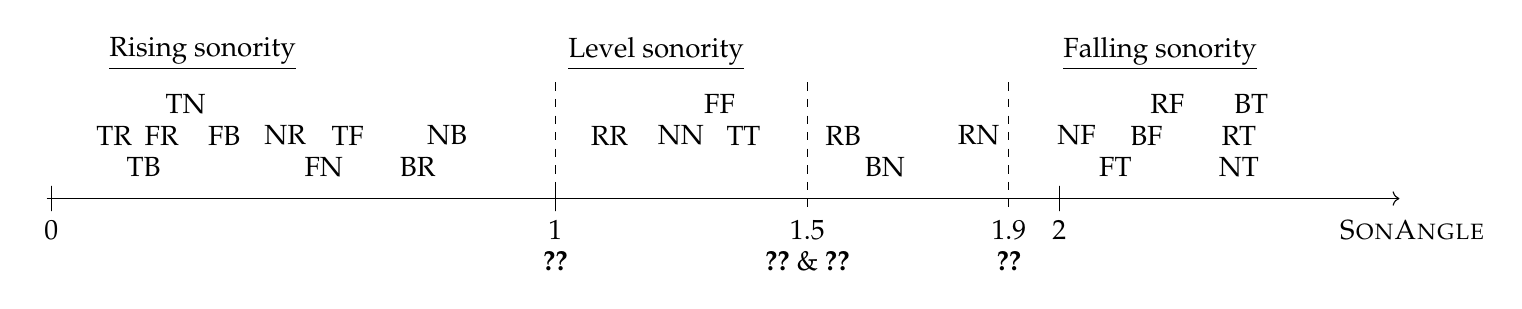
\begin{tikzpicture}[scale=0.8,shorten >=1pt,->]
  \tikzstyle{point}=[circle,fill=black!25,minimum size=12pt,inner sep=2pt]
  \tikzstyle{line} = [draw, -latex']

	\node (TR) at (0.124354994547*8, 1) {TR};
	\node (Tb) at (0.183110817262*8, 0.5) {T\textipa{B}};
	\node (FR) at (0.218668945874*8, 1) {FR};
	\node (TN) at (0.266252049151*8, 1.5) {TN};
	\node (Fb) at (0.343023940421*8, 1) {F\textipa{B}};
	\node (NR) at (0.463647609001*8, 1) {NR};
	\node (FN) at (0.540419500271*8, 0.5) {FN};
	\node (TF) at (0.588002603548*8, 1) {TF};
	\node (bR) at (0.726642340682*8, 0.5) {\textipa{B}R};
	\node (Nb) at (0.785398163397*8, 1) {N\textipa{B}};
	\node (RR) at (1.10714871779*8, 1) {RR};
%	\node (bb) at (1.19028994968*8, 0.5) {\textipa{BB}};
	\node (NN) at (1.2490457724*8, 1) {NN};
	\node (FF) at (1.32581766367*8, 1.5) {FF};
	\node (TT) at (1.37340076695*8, 1) {TT};
	\node (Rb) at (1.57079632679*8, 1) {R\textipa{B}};
	\node (bN) at (1.65393755868*8, 0.5) {\textipa{B}N};
	\node (RN) at (1.84*8, 1) {RN}; %1.89254688119
	\node (NF) at (2.0344439358*8, 1) {NF};
%	\node (GF) at (2.0344439358*8, 1.5) {GF};
	\node (FT) at (2.11121582707*8, 0.5) {FT};
	\node (bF) at (2.17308367293*8, 1) {\textipa{B}F};
	\node (RF) at (2.21429743559*8, 1.5) {RF};
	\node (RT) at (2.35619449019*8, 1) {RT};
	\node (NT) at (2.35619449019*8, 0.5) {NT};
	\node (bT) at (2.38057989937*8, 1.5) {\textipa{B}T};
  \node (rising) at (0.3*8,2.3) {\underline{Rising sonority}};
  \node (level) at (1.2*8,2.3) {\underline{Level sonority}};
  \node (falling) at (2.2*8,2.3) {\underline{Falling sonority}};
  % axis
  \node (axisstart) at (-0.23,0) {};
  \node (axisend)   at (2.7*8,0) {};
  \draw (axisstart) -- (axisend);
  \draw (0.0*8, 0.2) -- (0.0*8, -0.2) -- cycle;
  \draw (1.0*8, 0.2) -- (1.0*8, -0.2) -- cycle;
  \draw (2.0*8, 0.2) -- (2.0*8, -0.2) -- cycle;
  \node (0pointlabel) at (0.0,-0.5) {0};
  \node (1pointlabel) at (1.0*8,-0.5) {1};
  \node (2pointlabel) at (2.0*8,-0.5) {2};
  \node (xaxislabel) at (2.7*8,-0.5) {\textsc{SonAngle}};
  % dividing line
  \node (dividinglinestart) at (1.9 * 8,2) {};
  \node (dividinglineend)   at (1.9 * 8,-0.3) {};
  \path [line,dashed] (dividinglinestart) -- (dividinglineend) -- cycle;
  \node (dividingpointlabel) at (1.9*8, -0.5) {1.9};
  \node (dividingpointlabel2) at (1.9*8, -1.0) {\ref{CRNidiolect}};
  % another dividing line
  \node (dividingline2start) at (1.5 * 8,2) {};
  \node (dividingline2end)   at (1.5 * 8,-0.3) {};
  \path [line,dashed] (dividingline2start) -- (dividingline2end) -- cycle;
  \node (dividingpoint2label) at (1.5*8, -0.5) {1.5};
  \node (dividingpoint2label2) at (1.5*8, -1.0) {\ref{defaultCCCidiolect} \& \ref{C1CCidiolect}};
  % third dividing line
  \node (dividingline3start) at (1.0 * 8,2) {};
  \node (dividingline3end)   at (1.0 * 8,-0.3) {};
  \node (dividingpoint3label) at (1.0*8, -1.0) {\ref{wizfidiolect}};
  \path [line,dashed] (dividingline3start) -- (dividingline3end) -- cycle;
  
\end{tikzpicture}
}

\bigskip
The {\sc Sonority Rise} metric can achieve the same linear separation for idiolects \ref{defaultCCCidiolect}, \ref{C1CCidiolect} and \ref{wizfidiolect}, but notice that this is not possible for idiolect \ref{CRNidiolect}, because {\sc Sonority Rise} cannot achieve a linear separation of the sonority rises, plateaus and RN from the remainder of the falling sonority clusters.

\bigskip
\resizebox{\linewidth}{!}{
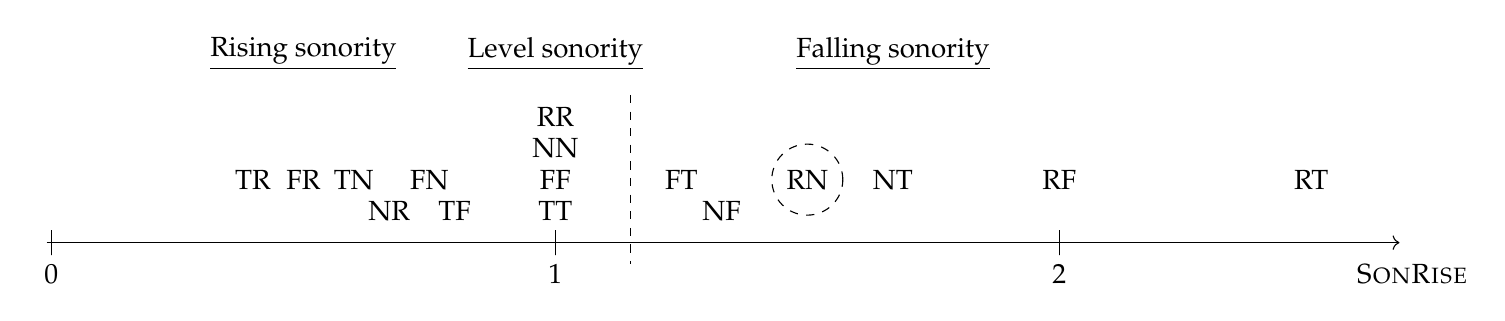
\begin{tikzpicture}[scale=0.8,shorten >=1pt,->]
  \tikzstyle{line} = [draw, -latex']
  \node (RT) at (2.5*8, 0)  {RT};
  \node (NT) at (1.67*8,0)  {NT};
  \node (FT) at (1.25*8,0)  {FT};
  \node (TT) at (1*8,-0.5)     {TT};
  \node (RF) at (2*8,0)     {RF};
  \node (NF) at (1.33*8,-0.5)  {NF};
  \node (FF) at (1*8,0)   {FF};
  \node (TF) at (0.8*8,-0.5)   {TF};
  \node[draw,circle,dashed] (RN) at (1.5*8,0)   {RN};
  \node (NN) at (1*8,0.5)     {NN};
  \node (FN) at (0.75*8,0)  {FN};
  \node (TN) at (0.6*8,0)   {TN};
  \node (RR) at (1*8,1.0)  {RR};
  \node (NR) at (0.67*8,-0.5)  {NR};
  \node (FR) at (0.5*8,0)   {FR};
  \node (TR) at (0.4*8,0)   {TR};
  \node (rising) at (0.5*8,2) {\underline{Rising sonority}};
  \node (level) at (1*8,2) {\underline{Level sonority}};
  \node (falling) at (1.67*8,2) {\underline{Falling sonority}};
  % axis
  \node (axisstart) at (-0.23,-1.0) {};
  \node (axisend)   at (2.7*8,-1.0) {};
  \draw (axisstart) -- (axisend);
  \draw (0.0*8, -1.2) -- (0.0*8, -0.8) -- cycle;
  \draw (1.0*8, -1.2) -- (1.0*8, -0.8) -- cycle;
  \draw (2.0*8, -1.2) -- (2.0*8, -0.8) -- cycle;
  \node (0pointlabel) at (0.0,-1.5) {0};
  \node (1pointlabel) at (1.0*8,-1.5) {1};
  \node (2pointlabel) at (2.0*8,-1.5) {2};
  \node (xaxislabel) at (2.7*8,-1.5) {\textsc{SonRise}};

  % third dividing line
  \node (dividingline3start) at (1.15 * 8,1.5) {};
  \node (dividingline3end)   at (1.15 * 8,-1.5) {};
  \path [line,dashed] (dividingline3start) -- (dividingline3end) -- cycle;
\end{tikzpicture}
}
\bigskip

\citet{rose.2000} presents a successful analysis of the same data in Chaha, from which I have liberally borrowed. Under her approach, it is Syllable Contact that triggers epenthesis. To this end, she employs two versions of Syllable Contact that achieve the grouping effect above. The first permits sonority falls, while the second, looser constraint, permits both sonority falls and plateaus.

\ex. \a. {\sc SyllCon}: The first segment of the onset of a syllable must be lower in sonority  \citep[(5)]{rose.2000}
     \b. {\sc SyllCon(Loose}): The first segment of the onset of a syllable must not be of greater sonority than the last segment of the immediately preceding syllable. \citep[(49)]{rose.2000}

Variable placement of these two constraints with respect to {\sc Align-Left} and {\sc Anchor-Left Root}, which themselves can be variably ranked, predict three of the four idiolects.

\ex. Rose's constraint rankings for idiolects \ref{defaultCCCidiolect}, \ref{C1CCidiolect} and \ref{wizfidiolect}.
    \a. Idiolect \ref{defaultCCCidiolect}: {\sc SyllCon} $\gg$ {\sc Dep} $\gg$ {\sc Align-L} $\gg$ {\sc Anchor-L Root}
          \a. $[$CC\textipa{1}C$]$ unless C\textsubscript{1}C\textsubscript{2} violates {\sc SyllCon}
               (is a sonority rise or plateau) and C\textsubscript{2}C\textsubscript{3} would not.
          \z.
     \b. Idiolect \ref{C1CCidiolect}: {\sc SyllCon} $\gg$ {\sc Dep} $\gg$ {\sc Anchor-L Root} $\gg$ {\sc Align-L} 
          \a.  $[$C\textipa{1}CC$]$ unless C\textsubscript{2}C\textsubscript{3} violates {\sc SyllCon}
                (is a sonority rise or plateau) and C\textsubscript{1}C\textsubscript{2} would not.
          \z.
     \c. Idiolect \ref{wizfidiolect}: {\sc SyllCon(Loose)} $\gg$ {\sc Dep} $\gg$ {\sc Anchor-L Root} $\gg$ {\sc Align-L} $\gg$ {\sc SyllCon}
          \a. $[$C\textipa{1}CC$]$ unless C\textsubscript{2}C\textsubscript{3} violates {\sc SyllCon(Loose)} 
                (is a sonority rise) and C\textsubscript{1}C\textsubscript{2} would not.
          \z.

Thus far, the logic has been very similar to the {\sc Sonority Angle} analysis. Explaining the special behaviour of RN clusters in the [CR\textipa{1}N] idiolect \ref{CRNidiolect}, requires invoking the {\sc *R-Son} constraint used in the analysis of idiolects \ref{idiolectb} and \ref{idiolectd} of the coda clusters.

\ex. Rose's constraint ranking for the [CR\textipa{1}N] idiolect \ref{CRNidiolect}
     \a. {\sc *R-Son} $\gg$ {\sc SyllCon} $\gg$ {\sc Dep} $\gg$ {\sc Align-L} $\gg$ {\sc Anchor-L Root}

In addition to these, the {\sc *MedialLight} constraint from Rose's analysis of the medial two-consonant clusters must again be invoked to prevent double epenthesis forming [C\textipa{1}C\textipa{1}C] in the case where both C\textsubscript{1}C\textsubscript{2} and C\textsubscript{2}C\textsubscript{3} constitute violations of {\sc SyllCon}.

% comment on need for *CCC?

\subsection{CCCC clusters}

In this last part of our case study of Chaha, we turn to the behaviour of quadriconsonantal clusters. The only such clusters come from the imperative/jussive CCC stem followed by the consonant-initial suffix -\textipa{n@}. The underlying form is /\textipa{n-\textnormal{CCC}-n@}/. They surface either as [\textipa{n1\underline{\textnormal{CC}1\textnormal{C}n}@}] or [\textipa{n1\underline{\textnormal{C}1\textnormal{CC}1n}@}].

In this section, I will demonstrate that the four rankings already obtained in $\S$\ref{CCCanalysis} for the triconsonantal clusters generalise without modification to the CCCC clusters, predicting almost exactly which of the quadriconsonantal clusters should display variation, and in which direction.

\subsubsection{Data}

The following table shows the observed behaviour of the quadriconsonantal clusters of Chaha, as reported by \cite{rose.2000}.

\ex. Epenthetic behaviour of CCCC clusters

\vspace{-2em}
\begin{center}
\begin{longtable}{|cc|c|} \hline
   & Underlying form & Observed surface forms \\ \hline
 a.& \textipa{n-sdB-n@} & \textipa{n1sd1Bn@} \\ 
 b.& \textipa{n-wzf-n@} & \textipa{n1wz1fn@}, \textipa{n1w1zf1n@} \\
 c.& \textipa{n-gdf-n@} & \textipa{n1gd1fn@}, \textipa{n1g1df1n@} \\
 d.& \textipa{n-mst-n@} & \textipa{n1m1st1n@} \\
 e.& \textipa{n-dmd-n@} & \textipa{n1d1md1n@} \\
 f.& \textipa{n-drs-n@} & \textipa{n1d1rs1n@} \\
 g.& \textipa{n-sBx-n@} & \textipa{n1s1Bx1n@} \\
 h.& \textipa{n-kft-n@} & \textipa{n1k1ft1n@}  \\
 i.& \textipa{n-ktf-n@} & \textipa{n1kt1fn@}, \textipa{n1k1tf1n@} \\
 j.& \textipa{n-sgd-n@} & \textipa{n1sg1dn@}, \textipa{n1s1gd1n@} \\
 k.& \textipa{n-srB-n@} & \textipa{n1sr1Bn@}, \textipa{n1s1rB1n@} \\
 l.& \textipa{n-krm-n2} & \textipa{n1kr1mn@}, \textipa{n1k1rm1n@}  \\ 
 m.& \textipa{n-nk'm-n@}& \textipa{n1nk'1mn@} \\
 n.& \textipa{n-nfk-n@} & \textipa{n1nf1kn@} \\
 o.& \textipa{n-rmd-n@} & \textipa{n1rm1dn@} \\ 
 p.& \textipa{n-k'ff-n@} & \textipa{n1k'f1fn@} \\
 q.& \textipa{n-sdd-n@}  & \textipa{n1sd1dn@} \\ \hline
 \end{longtable}
\end{center}

\vspace{-2em}

\subsubsection{Predictions of CCC rankings}

The undominated nature of the constraint *CCC, which we used to trigger epenthesis among the triconsonantal clusters, also triggers epenthesis in quadriconsonantal clusters.
This excludes possible solutions such as *[C\textipa{1}CCC] and *[CCC\textipa{1}C], as these still incur a violation of *CCC.

Solutions such as [C\textipa{1}C\textipa{1}CC] and [CC\textipa{1}C\textipa{1}C] are also excluded, as these incur unnecessary violations of {\sc Ident(Son$\measuredangle$)} and {\sc Dep}. If the middle two consonants C\textsubscript{2} and C\textsubscript{3} are split up by an epenthetic vowel, there is no further need for epenthesis as *CCC is already satisfied by [CC\textipa{1}CC].

Therefore, the only two possible solutions under my approach are [CC\textipa{1}CC] and [C\textipa{1}CC\textipa{1}C]. Which one is chosen depends on the sonority profile of the clusters, and which of Rose's constraints {\sc Align-Left} and {\sc Anchor-Left Root} is dominant.

\ex. {\sc Align-Left} favours [CC\textipa{1}CC], but {\sc Anchor-Left Rt} favours [C\textipa{1}CC\textipa{1}C].
\vspace{-1em}
\begin{center} \renewcommand*\arraystretch{1.2}
\scalebox{1}[1]{\begin{tabular}[t]{|rrl||c:c|} \hline 
\multicolumn{3}{|c||}{Input:~/\textipa{n-\textnormal{CCC}-n@}/} & {\sc Align-Left} & {\sc Anchor-Left Rt} \\[0.5ex]
\hline \hline a. & & \textipa{n1\textnormal{C.C}1\textnormal{C}.n@} & 2,3,5,6 & $\ast$! \\
\hline b. & \ding{43} & \textipa{n1.\textnormal{C}1\textnormal{C.C}1.n@} & 2,4!,5,7 & \\
\hline \end{tabular}} \renewcommand*\arraystretch{1} \end{center}

There are some clusters whose epenthetic behaviour is subject to other considerations. The constraint {\sc Jussive-R} still applies to these forms, for example, which ensures that the following forms epenthesise as [CC\textipa{1}CC]:

\ex. \a. \textipa{n1-\underline{nk'1m-n}@}
     \b. \textipa{n1-\underline{nf1k-n}@}
     \c. \textipa{n1-\underline{rm1d-n}@}
     \z. \citep[(33a,34a,34b)]{rose.2000}

In addition, Chaha prohibits intramorphemic geminates, which enforces the following forms:

\ex. \a. \textipa{n1-\underline{k'f1fn}@}
     \b. \textipa{n1-\underline{sd1dn}@}
     \z. \citep[(37a,b)]{rose.2000}

I will not consider such clusters further.

\bigskip

Given the general form of the ranking {\sc Ident(Son$\measuredangle$)}$<$n $\gg$ {\sc Align-Left} $\gg$ {\sc Anchor-Left Root}, the expected behaviour of four-consonant clusters is as follows: all /CCCC/ clusters surface as [CC\textipa{1}CC], except when {\sc SonAngle}(C\textsubscript{2},C\textsubscript{3}) exceeds n and {\sc SonAngle}(C\textsubscript{1},C\textsubscript{2}) and {\sc SonAngle}(C\textsubscript{3},C\textsubscript{4}) are both smaller than n. Illustrative tableaux are shown below for n=1.5:

\ex. {\sc Ident(Son$\measuredangle$)}$<$1.5 $\gg$ {\sc Align-Left}
\vspace{-0.5em}
     \a. Case 1: {\sc Sonority Angle}(C\textsubscript{2},C\textsubscript{3})$<$1.5
\begin{center} \renewcommand*\arraystretch{1.2}
\scalebox{1}[1]{\begin{tabular}[t]{|rrl||c|c|} \hline 
\multicolumn{3}{|c||}{Input:~/\textipa{n-gdf-n@}/} & {\sc Ident(Son$\measuredangle$)}$<$1.5 & {\sc Align-Left} \\[0.5ex]
\hline \hline a. & \ding{43} & \textipa{n1gd1fn@} & 0.59 & \\
\hline b. & & \textipa{n1g1df1n@} & 1.37, 0.54 & $\ast$! \\
\hline \end{tabular}} \renewcommand*\arraystretch{1} \end{center}
\vspace{0.5em}
     \b. Case 2: {\sc Sonority Angle}(C\textsubscript{2},C\textsubscript{3})$>=$1.5 but so is one of {\sc Sonority Angle}(C\textsubscript{1},C\textsubscript{2}) or {\sc Sonority Angle}(C\textsubscript{3},C\textsubscript{4})
\vspace{-0.5em}
\begin{center} \renewcommand*\arraystretch{1.2}
\scalebox{1}[1]{\begin{tabular}[t]{|rrl||c|c|} \hline 
\multicolumn{3}{|c||}{Input:~/\textipa{n-srB-n@}/} & {\sc Ident(Son$\measuredangle$)}$<$1.5 & {\sc Align-Left} \\[0.5ex] 
\hline \hline c. & \ding{43} & \textipa{n1sr1Bn@} & 1.57 $\ast$ &  \\
\hline d. & & \textipa{n1s1rB1n@} & 0.22, 1.65$\ast$ & $\ast$! \\
\hline \end{tabular}} \renewcommand*\arraystretch{1} \end{center}
\vspace{0.5em}
      \c. Case 3: {\sc Sonority Angle}(C\textsubscript{2},C\textsubscript{3})$>=$1.5 and both {\sc Sonority Angle}(C\textsubscript{1},C\textsubscript{2}) and {\sc Sonority Angle}(C\textsubscript{3},C\textsubscript{4})$<$1.5
\vspace{-0.5em}
\begin{center} \renewcommand*\arraystretch{1.2}
\scalebox{1}[1]{\begin{tabular}[t]{|rrl||c|c|} \hline 
\multicolumn{3}{|c||}{Input:~/\textipa{n-dmd-n@}/} & {\sc Ident(Son$\measuredangle$)}$<$1.5 & {\sc Align-Left} \\[0.5ex]
\hline \hline e. &  & \textipa{n1dm1dn@} & 2.3 $\ast$!   & \cellcolor{lightgray} \\
\hline f. & \ding{43} & \textipa{n1d1md1n@} & 0.27, 0.27 & \cellcolor{lightgray} $\ast$ \\
\hline \end{tabular}} \renewcommand*\arraystretch{1} \end{center}

\bigskip

Given the general form of the ranking {\sc Ident(Son$\measuredangle$)}$<$n $\gg$ {\sc Anchor-Left Root} $\gg$ {\sc Align-Left}, the default behaviour is to epenthesise as [C\textipa{1}CC\textipa{1}C]. This preference is overridden when at least one of {\sc SonAngle}(C\textsubscript{1},C\textsubscript{2}) and {\sc SonAngle}(C\textsubscript{3},C\textsubscript{4}) are greater than n and {\sc SonAngle}(C\textsubscript{2},C\textsubscript{3}) is less than n.

\newpage
\ex. {\sc Ident(Son$\measuredangle$)}$<$1.5 $\gg$ {\sc Anchor-Left Rt}
     \a. Case 1: Both {\sc Sonority Angle}(C\textsubscript{1},C\textsubscript{2}) and {\sc Sonority Angle}(C\textsubscript{3},C\textsubscript{4})$<$1.5
\vspace{-0.5em}
\begin{center} \renewcommand*\arraystretch{1.2}
\scalebox{1}[1]{\begin{tabular}[t]{|rrl||c|c|} \hline 
\multicolumn{3}{|c||}{Input:~/\textipa{n-gdf-n@}/} & {\sc Ident(Son$\measuredangle$)}$<$1.5 & {\sc Anchor-Left Rt} \\[0.5ex]
\hline \hline a. &  & \textipa{n1gd1fn@} & 0.59 & $\ast$!\\
\hline b. & \ding{43} & \textipa{n1g1df1n@} & 1.37, 0.54 &  \\
\hline \end{tabular}} \renewcommand*\arraystretch{1} \end{center}
\vspace{0.5em}
     \b. Case 2: {\sc Sonority Angle}(C\textsubscript{1},C\textsubscript{2}) or {\sc Sonority Angle}(C\textsubscript{3},C\textsubscript{4}) $>=$1.5, but so is {\sc Sonority Angle}(C\textsubscript{2},C\textsubscript{3})
\vspace{-0.5em}
\begin{center} \renewcommand*\arraystretch{1.2}
\scalebox{1}[1]{\begin{tabular}[t]{|rrl||c|c|} \hline 
\multicolumn{3}{|c||}{Input:~/\textipa{n-srB-n@}/} & {\sc Ident(Son$\measuredangle$)}$<$1.5 & {\sc Anchor-Left Rt} \\[0.5ex]
\hline \hline c. &  & \textipa{n1sr1Bn@} & 1.57 $\ast$ & $\ast$! \\
\hline d. & \ding{43} & \textipa{n1s1rB1n@} & 0.22, 1.65$\ast$ &  \\
\hline \end{tabular}} \renewcommand*\arraystretch{1} \end{center}
\vspace{0.5em}
     \c. Case 3: {\sc Sonority Angle}(C\textsubscript{1},C\textsubscript{2}) or {\sc Sonority Angle}(C\textsubscript{3},C\textsubscript{4}) $>=$1.5, and {\sc Sonority Angle}(C\textsubscript{2},C\textsubscript{3})$<$1.5
\vspace{-0.5em}
\begin{center} \renewcommand*\arraystretch{1.2}
\scalebox{1}[1]{\begin{tabular}[t]{|rrl||c|c|} \hline 
\multicolumn{3}{|c||}{Input:~/\textipa{n-sdB-n@}/} & {\sc Ident(Son$\measuredangle$)}$<$1.5 & {\sc Anchor-Left Rt} \\[0.5ex]
\hline \hline a. & \ding{43} & \textipa{n1sd1Bn@} & 0.18 & \cellcolor{lightgray} $\ast$ \\
\hline b. & & \textipa{n1s1dB1n@} & 2.11 $\ast$!, 1.65 $\ast$ & \cellcolor{lightgray} \\
\hline \end{tabular}} \renewcommand*\arraystretch{1} \end{center}


The following table shows the actual surface forms observed for each of the underlying clusters, as well as the predictions of the four idiolectal rankings. 

\ex. Table of CCCC clusters, observed outcomes and predictions made by the constraint rankings proposed for the four idiolects in $\S$\ref{CCCanalysis}.

\begin{center}
\begin{tabular}{|l|ccc|c|cccc|} \hline
         & \multicolumn{3}{c|}{{\sc SonAngles}} & Observed & \multicolumn{4}{c|}{{\sc Predictions of idiolect}} \\
 Cluster & C\textsubscript{1},C\textsubscript{2} & C\textsubscript{2},C\textsubscript{3} & C\textsubscript{3},C\textsubscript{4} &  outcomes & \ref{defaultCCCidiolect} & \ref{CRNidiolect} & \ref{C1CCidiolect} & \ref{wizfidiolect} \\ \hline 
 a. \textipa{sdBn} & 2.11 & 0.18 & 1.66 & \textipa{sd1Bn} & \multicolumn{4}{c|}{\textipa{sd1Bn}} \\ 
 b. \textipa{wzfn} & 2.03 & 1.33 & 0.54 & \textipa{wz1fn}, \textipa{w1zf1n} & \multicolumn{3}{c}{\textipa{wz1fn}} & \cellcolor{lightgray}  \textipa{w1zf1n} \\
 c. \textipa{gdfn} & 1.37 & 0.59 & 0.54 & \textipa{gd1fn}, \textipa{g1df1n} & \multicolumn{2}{c}{\textipa{gd1fn}} & \cellcolor{lightgray}  \textipa{g1df1n} &  \textipa{gd1fn} \\
 d. \textipa{mstn} & 2.03 & 2.11 & 0.27 & \textipa{m1st1n} & \multicolumn{2}{c}{*\textipa{ms1tn}} & \multicolumn{2}{c|}{\cellcolor{lightgray}  \textipa{m1st1n}} \\
 e. \textipa{dmdn} & 0.27 & 2.36 & 0.27 & \textipa{d1md1n} & \multicolumn{4}{c|}{\cellcolor{lightgray} \textipa{d1md1n}} \\
 f. \textipa{drsn} & 0.12 & 2.21 & 0.54 & \textipa{d1rs1n} & \multicolumn{4}{c|}{\cellcolor{lightgray} \textipa{d1rs1n}} \\
 g. \textipa{sBxn} & 0.34 & 2.17 & 0.54 & \textipa{s1Bx1n} & \multicolumn{4}{c|}{\cellcolor{lightgray} \textipa{s1Bx1n}} \\
 h. \textipa{kftn} & 0.59 & 2.11 & 0.27 & \textipa{k1ft1n} & \multicolumn{4}{c|}{\cellcolor{lightgray} \textipa{k1ft1n}} \\
 i. \textipa{ktfn} & 1.37 & 0.59 & 0.54 & \textipa{kt1fn}, \textipa{k1tf1n} & \multicolumn{2}{c}{\textipa{kt1fn}} & \cellcolor{lightgray}  \textipa{k1tf1n} &  \textipa{kt1fn} \\
 j. \textipa{sgdn} & 2.11 & 1.37 & 0.27 & \textipa{sg1dn}, \textipa{s1gd1n} & \multicolumn{3}{c}{\textipa{sg1dn}} & \cellcolor{lightgray}  \textipa{s1gd1n} \\
 k. \textipa{srBn} & 0.22 & 1.57 & 1.65 & \textipa{sr1Bn}, \textipa{s1rB1n} & \multicolumn{2}{c}{\textipa{sr1Bn}} & \multicolumn{2}{c|}{\cellcolor{lightgray}  \textipa{s1rB1n}} \\
 l. \textipa{krmn} & 0.12 & 1.89 & 1.25 & \textipa{kr1mn}, \textipa{k1rm1n} & \cellcolor{lightgray}  \textipa{k1rm1n} & \textipa{kr1mn} & \multicolumn{2}{c|}{\cellcolor{lightgray}  \textipa{k1rm1n}} \\ \hline
 \end{tabular}
\end{center}

\newpage

There is only one incorrect prediction, namely that /mstn/ should surface as [\textipa{ms1tn}] in idiolects \ref{defaultCCCidiolect} and \ref{CRNidiolect}, but Rose indicates that there is no variation in this form. It is possible that this is simply a form that does undergo variation but the predicted [\textipa{ms1tn}] variant has not been observed in Rose's corpus.

Apart from the case of /mstn/, we see that the predictions of the rankings derived for the /CCC/ case are quite successful: clusters predicted to show variation do show variation, while for those predicted to surface only as one of [CC\textipa{1}CC] and [C\textipa{1}CC\textipa{1}C], the predicted form is indeed the only one observed.

\subsection{Interim summary}

In this case study, I presented an alternative analysis of Chaha epenthetic positioning to \citet{rose.2000}'s Syllable Contact-based analysis, in which sonority profiles affected epenthesis via the mechanism of sonority-based faithfulness constraints {\sc Ident(Son$\measuredangle$)}$<$n rather than sonority-based markedness constraints such as Syllable Contact and Sonority Sequencing. The fact that general constraints on syllable structure such as *CCC and {\sc *ComplexCoda} drove epenthesis eliminated the need for constraints forbidding too much epenthesis, as Rose does in the form of the constraint {\sc *MedialLight}.

The prediction of {\sc Sonority Angle} that RN clusters should be the most susceptible of all the falling sonority clusters to epenthesis was borne out in the Chaha data, both in CC\# and CCC clusters. This fact made it possible for us to do without Rose's {\sc *R-Son} constraint, although at the expense of requiring a constraint against [\textipa{Bm}] clusters. Invoking another faithfulness constraint, {\sc Dep}(+son), in the analysis of CC\# clusters allowed us to eliminate the use of Rose's {\sc *C-Son} constraint, which also needed to make special reference to [r].

The more complex case of Chaha three- and four-consonant clusters also revealed that the {\sc Ident(Son$\measuredangle$)}$<$n constraints must be freely-rankable rather than fixed in a universal ranking. This allowed for faithfulness conflation of clusters both above and below a markedness constraint.

In the final tally, the {\sc Sonority Angle}-based approach fares worse on one datapoint and uses approximately the same number of constraints, but manages to accomplish most of the work of the analysis by ranking a single {\sc Ident(Son$\measuredangle$)}$<$n constraint with respect to a relevant $\mathcal{M}$ constraint, while in Rose's analysis this work is spread over a number of different sonority-related constraints.

\section{Discussion} \label{issues}

In this paper, I proposed two desiderata for a metric of sonority contour distance, and suggested {\sc Sonority Angle} as a concrete metric that fit these criteria. In this section, I examine first a general question regarding sonority contour faithfulness, then discuss weaknesses of {\sc Sonority Angle} as a metric, as well as possible extensions of this metric to domains beyond sonority-driven epenthesis.


\subsection{Disregarding VC\textsubscript{2}} 

In the sonority contour faithfulness approach, the relevant comparison is between C\textsubscript{1}C\textsubscript{2} and C\textsubscript{1}V. But why these two vectors? In particular, why not C\textsubscript{1}C\textsubscript{2} versus VC\textsubscript{2}?

\ex. Left: {\sc Sonority Angle} as currently defined; right: another possible definition as the angle C\textsubscript{1}C\textsubscript{2}-V.

\vspace{-1em} \hspace{1.5in}
\begin{tikzpicture} [scale=0.33]
  \draw [<-] (-3,6.5) -- (-3, 0.5) ; % axis
  \node at (-3, 7.0) {Sonority}; % axis label
  % left diagram
    \coordinate (A) at (0,3);
    \coordinate (B) at (5,1);
    \coordinate (C) at (5,6);
  \draw (B) -- (A) -- (C) ; % rising sonority
  \node[left] at  (A) {C$_1$}; 
  \node[right] at (B) {C$_2$};
  \node[right] at (C) {V};
\tkzMarkAngle[size=1.5cm](B,A,C)
\tkzLabelAngle[pos=2](B,A,C){$\theta$}

% right diagram
    \coordinate (D) at (15,3);
    \coordinate (E) at (20,1);
    \coordinate (F) at (15,6);
    \draw (D) -- (E) -- (F) ; % falling sonority
    \node[left] at (D) {C$_1$}; 
    \node[right] at (E) {C$_2$};
    \node[right] at (F) {V};
\tkzMarkAngle[size=2.5cm](F,E,D)
\tkzLabelAngle[pos=3](D,E,F){$\theta$}
\end{tikzpicture} 
\bigskip

The answer, currently, is based purely on empirical grounds: if we assume this comparison to be the relevant one, then we expect falling sonority contours to be more susceptible to epenthesis, which contradicts the cross-linguistic evidence. It would seem that there is something quite fundamental about the comparison being centred around the offset of C\textsubscript{1} rather than the C\textsubscript{1}, which may arise out of perception or phonological processing.

For instance, it is well known that CV cues are much more robust than VC cues \citep{wright.2004}.
This could be the reason for the offset of the consonant vastly outweighing the onset in terms of importance. Other sources for this asymmetry are also possible.


\subsection{Robustness of the metric}

\noindent {\bf Changes in C\textsubscript{1}.} In the discussion of Chaha triconsonantal clusters in  $\S$\ref{CCCanalysis}, I glossed over how the metric should be computed if C\textsubscript{1} changes.
This was an issue in clusters such as /rfk/, which emerge as [nf\textipa{1}k] due to morphophonological processes. Ultimately, this was not an issue because the behaviour of all such clusters was independently determined by {\sc Jussive-R}, but this raises the question of how {\sc Sonority Angle} should be computed if C\textsubscript{1} changes. Currently, it is undefined, as it is unclear how to measure the angle between C\textsubscript{1}C\textsubscript{2}=RF and C\textsubscript{1}V=NV (shown below on the left). A similar situation arises if C\textsubscript{1}C\textsubscript{2}=NF and C\textsubscript{1}V=FV (shown on the right):

\ex. Two scenarios under which {\sc Sonority Angle} is not well-defined:

\begin{center}
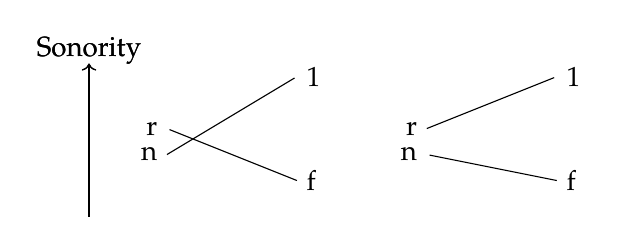
\begin{tikzpicture} [shorten >=1pt,scale=0.33]
                      \draw [<-] (-3,6.5) -- (-3, 0.5) ; % axis
                      \node at (-3, 7.0) {Sonority}; % axis label
					 % left diagram
                      \draw (5,2) -- (0,4);
                      \draw (0,3) -- (5,6) ; % rising sonority
                      \node[left] at  (0,4) {r}; 
                      \node[left] at  (0,3) {n}; 
                      \node[right] at (5,2) {f};
                      \node[right] at (5,6) {\textipa{1}};
                      \draw [<-] (-3,6.5) -- (-3, 0.5) ; % axis
                      \node at (-3, 7.0) {Sonority}; % axis label
					 % right diagram
                      \draw (15,2) -- (10,3);
                      \draw (10,4) -- (15,6) ; % rising sonority
                      \node[left] at  (10,3) {n}; 
                      \node[left] at  (10,4) {r}; 
                      \node[right] at (15,2) {f};
                      \node[right] at (15,6) {\textipa{1}};
\end{tikzpicture}
\end{center}

Several possibilities are possible: retain the sonority of the underlying C\textsubscript{1} for that of the output value; use the sonority of the output C\textsubscript{1} as the underlying value; or take the angle formed by the meeting of the two contours, wherever that occurs. 

\begin{center}
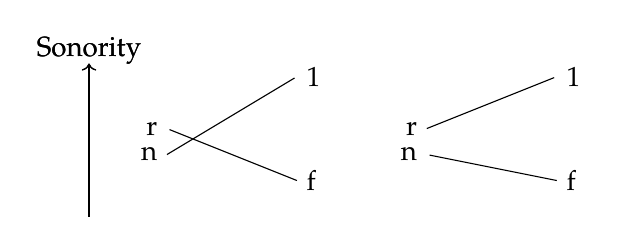
\begin{tikzpicture} [shorten >=1pt,scale=0.33]
                      \draw [<-] (-3,6.5) -- (-3, 0.5) ; % axis
                      \node at (-3, 7.0) {Sonority}; % axis label
					 % left diagram
                      \draw (5,2) -- (0,4);
                      \draw (0,3) -- (5,6) ; % rising sonority
                      \node[left] at  (0,4) {r}; 
                      \node[left] at  (0,3) {n}; 
                      \node[right] at (5,2) {f};
                      \node[right] at (5,6) {\textipa{1}};
                      \draw [<-] (-3,6.5) -- (-3, 0.5) ; % axis
                      \node at (-3, 7.0) {Sonority}; % axis label
					 % right diagram
                      \draw (15,2) -- (10,3);
                      \draw (10,4) -- (15,6) ; % rising sonority
                      \node[left] at  (10,3) {n}; 
                      \node[left] at  (10,4) {r}; 
                      \node[right] at (15,2) {f};
                      \node[right] at (15,6) {\textipa{1}};
\end{tikzpicture}
\end{center}

The case studies here constitute insufficient data to conclude if any of these interpretations is correct. It is worth noting, however, that alternative approaches such as {\sc Sonority Rise} do not face this issue, as computing the gradients of the underlying contour /C\textsubscript{1}C\textsubscript{2}/ and the surface contour [C\textsubscript{1}V] does not depend on the two C\textsubscript{1}'s being the same.

\bigskip

\noindent {\bf Choice of horizontal distance.} In this paper, I assumed that the horizontal distance between C\textsubscript{1} and C\textsubscript{2}, and C\textsubscript{1} and V, is the same, and arbitrarily fixed at 1 unit, in calculating {\sc Sonority Angle}. This is an arbitrary choice, and potentially an important one. While the horizontal distance is of a similar magnitude to the values of the sonority scale, the {\sc Sonority Angles} are more or less as we expect, but when the horizontal distance is made very large, changes occur in the cluster hierarchy, some of which violate the first desideratum for a sonority contour distance metric. While it is still true that keeping C\textsubscript{1} fixed, raising C\textsubscript{2} decreases the {\sc Sonority Angle} (compare TR vs TN vs TF vs TT, for example), we no longer have a linear separation of the three broad classes of sonority rises, sonority plateaus and sonority falls.

\ex. {\sc Sonority Angle} hierarchy for a horizontal distance of 100 units.

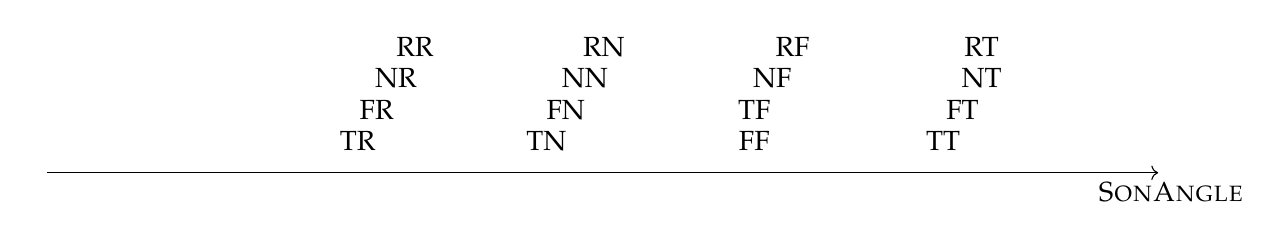
\begin{tikzpicture}[scale=0.8,shorten >=1pt,->]
  \node (RT) at (0.04998833883*300,1.5)   {RT};
  \node (NT) at (0.04998833883*300,1.0)  {NT};
  \node (FT) at (0.04897835381*300,0.5)  {FT}; %0.04997835381
  \node (TT) at (0.0479583957219*300,0)     {TT}; %0.0499583957219
  \node (RF) at (0.0399946679463*300,1.5)     {RF};
  \node (NF) at (0.038906715435*300,1.0)  {NF}; %0.0399906715435
  \node (TF) at (0.0379587290353*300,0.5)   {TF}; %0.0399587290353
  \node (FF) at (0.0379587290353*300,0)   {FF};%0.0399587290353
  \node (RN) at (0.0299970006598*300,1.5)   {RN};
  \node (NN) at (0.0289910048569*300,1.0)   {NN}; %0.0299910048569
  \node (FN) at (0.0279790204366*300,0.5)  {FN}; %0.0299790204366
  \node (TN) at (0.0269610617488*300,0)   {TN}; %0.0299610617488
  \node (RR) at (0.0199973339732*300,1.5)  {RR}; %
  \node (NR) at (0.0189913381702*300,1.0)  {NR}; %0.0199913381702
  \node (FR) at (0.0179813531501*300,0.5)   {FR};%0.0199813531501
  \node (TR) at (0.0169673908651*300,0)   {TR}; %0.0199673908651
  % axis
  \node (axisstart) at (0.0,-0.5) {};
  \node (axisend)   at (0.06*300,-0.5) {};
  \draw (axisstart) -- (axisend);
  \node  (0point) at (0.0,0) {};
  \node (xaxislabel) at (0.06*300,-0.8) {\textsc{SonAngle}};
\end{tikzpicture}

Notice that we cannot achieve a clean separation of the rising versus level versus falling sonority clusters, as before. Compare this with {\sc Sonority Rise} which, being dimensionless (since it is the ratio of two vectors in the same plane), does not have to take into account such units.

Additionally, since this horizontal distance is along the dimension of time, the assumption that the two horizontal distance for C\textsubscript{1}C\textsubscript{2} is the same as that for C\textsubscript{1}V is likely incorrect. If we choose different values for these two horizontal distances, the cluster hierarchy would also be likely to change. This would also be a consideration to take into account when computing {\sc Sonority Rise}.

\bigskip

\noindent {\bf Choice of sonority scale.} A third issue faced by any sonority metric is the arbitrariness of the vertical, sonority scale used in this paper. The scale adopted, which is a relatively standard scale, is rather phonological in nature, placing each sonority class at a distance of 1 from the next, and ignoring all differences between consonants within each class. From a phonetic standpoint, this seems unlikely.

Perhaps the closest thing we have to a phonetic sonority scale comes from \citet{parker.2002}, who measured various acoustic correlates of sonority and showed that phonological sonority correlates to a very high degree with intensity ({\it r} = .97--.99).

\ex. Intensity data for English males (in dB) \citep[Table 5.13]{parker.2002}\footnote{The intensity values measured for the three vowel classes are reversed from what one would expect according to phonological sonority \citep[214]{parker.2002}}, but overall this shows a good correlation with scales of phonological sonority. The distinction between some of these classes is not significant, including between the high and mid vowels.

\begin{center}
\begin{tabular}{cc}
 Segments & Mean \\ \hline
 \textipa{i I u U} & 10.65 \\
 \textipa{e E 2 o O} & 10.21 \\
 \textipa{\ae  a} & 9.62 \\
 \textipa{@} &  5.73 \\
 \textipa{y w} & 3.92 \\
 \textipa{r} & 2.53 \\
 \textipa{l} & 2.51 \\
 \textipa{m n} & -4.16 \\
 \textipa{h} & -6.05 \\
 \textipa{v D z Z} & -6.30 \\
 \textipa{P} & -11.10 \\
 \textipa{f T s S} & -11.96 \\
 \textipa{b d g dZ} & -12.41 \\
 \textipa{p t k tS} & -13.75 \\  
\end{tabular}	
\end{center}

Plugging these numbers into the {\sc Sonority Angle} metric and using an average of the values of the vowel and averaging together voiced and voiceless members of the same class, we obtain the following hierarchy of clusters:

\ex. {\sc Sonority Angle} cluster hierarchy obtained using Parker's intensity data for English males, averaging [$\pm$voice] values for obstruent classes.

\bigskip
\resizebox{\linewidth}{!}{
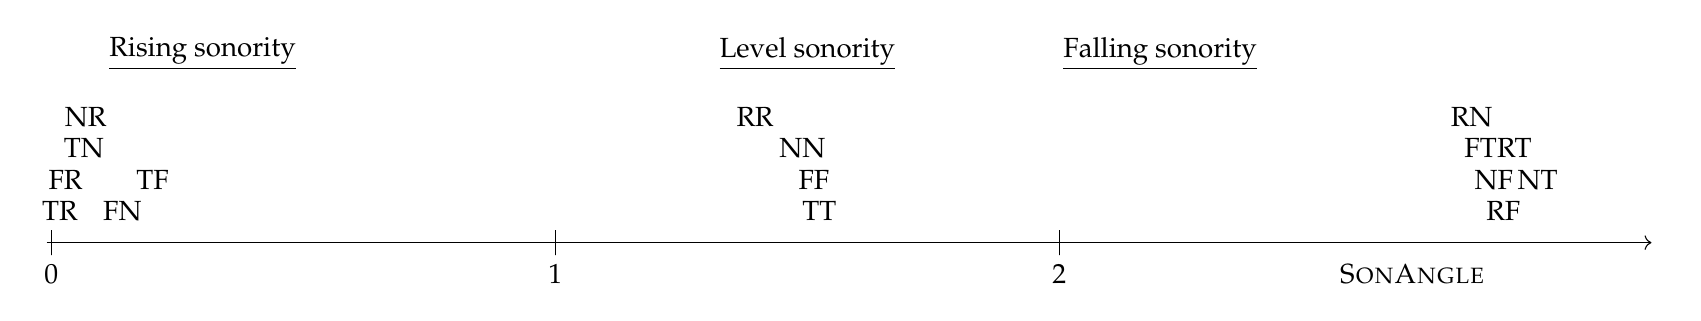
\begin{tikzpicture}[scale=0.8,shorten >=1pt,->]
  \tikzstyle{point}=[circle,fill=black!25,minimum size=12pt,inner sep=2pt]
  \tikzstyle{line} = [draw, -latex']

\node (TR) at (0.0170349973202*8, 0.5) {TR};
	\node (FR) at (0.0279543293301*8, 1) {FR};
	\node (TN) at (0.0646614923105*8, 1.5) {TN};
	\node (NR) at (0.0678017301617*8, 2.0) {NR};
	\node (FN) at (0.140883408022*8, 0.5) {FN};
	\node (TF) at (0.200974864302*8, 1.0) {TF};
	\node (RR) at (1.39622474153*8, 2) {RR};
	\node (NN) at (1.49000093511*8, 1.5) {NN};
	\node (FF) at (1.5131236339*8, 1) {FF};
	\node (TT) at (1.52381634628*8, 0.5) {TT};
	\node (RN) at (2.81842394648*8, 2) {RN};
	\node (FT) at (2.83596511588*8, 1.5) {FT};
	\node (NF) at (2.86224116099*8, 1) {NF};
	\node (RF) at (2.8813940461*8, 0.5) {RF};
	\node (RT) at (2.90300609049*8, 1.5) {RT};
	\node (NT) at (2.94915578908*8, 1) {NT};
	
  \node (rising) at (0.3*8,3) {\underline{Rising sonority}};
  \node (level) at (1.5*8,3) {\underline{Level sonority}};
  \node (falling) at (2.2*8,3) {\underline{Falling sonority}};
  % axis
  \node (axisstart) at (-0.23,0) {};
  \node (axisend)   at (3.2*8,0) {};
  \draw (axisstart) -- (axisend);
  \draw (0.0*8, 0.2) -- (0.0*8, -0.2) -- cycle;
  \draw (1.0*8, 0.2) -- (1.0*8, -0.2) -- cycle;
  \draw (2.0*8, 0.2) -- (2.0*8, -0.2) -- cycle;
  \node (0pointlabel) at (0.0,-0.5) {0};
  \node (1pointlabel) at (1.0*8,-0.5) {1};
  \node (2pointlabel) at (2.0*8,-0.5) {2};
  \node (xaxislabel) at (2.7*8,-0.5) {\textsc{SonAngle}};
\end{tikzpicture}
}

Using this scale, we obtain the desired empirical results of this paper based on the evidence of Irish and Chaha, that RN is the most epenthesisable of all the falling sonority clusters and that RT and NT are the clusters most resistant to epenthesis. However, this does not conform to the general principle that for a given sonority distance, the more sonorous the consonants, the more likely a cluster is to undergo epenthesis --- we have NF being harder to epenthesise into than FT, here.

Moreover, this result is obtained by averaging stops and fricatives to ignore voicing. If we leave voicing intact, then these results disappear: fricative--voiceless stops are the most likely to undergo epenthesis of the falling sonority clusters, more so than liquid--nasal clusters, and if RT and NT fail to undergo epenthesis, we expect voiced fricative--voiced stop, nasal--voiceless fricative, and nasal--voiced stop clusters to also resist epenthesis. Both of these are contrary to the empirical results of this paper.

\bigskip

Ultimately, the most practical course of action may be to simply attempt to experimentally determine sonority contour distances through a perceptual experiment, then fit them to a metric based on a suitable sonority scale. To date, only a few sonority contour distances have been experimentally determined, for example between rising (TR) and falling (sT) clusters \citep{fleischhacker.2002}, but not finer-grained distances such as between the various falling sonority clusters. I leave this to future work.

\subsection{Extensions of the metric}

So far, I have employed the {\sc Sonority Angle} metric purely in the analysis of sonority-driven epenthesis. However, there are other possible applications.

\bigskip

\noindent {\bf Syncope.} We can straightforwardly adapt the sonority contour faithfulness account to analyse syncope, as pointed out by \citet{flemming.2008}. Interestingly, this makes different predictions from an account based on Syllable Contact, unlike the case of epenthesis where sonority contour faithfulness and Syllable Contact make similar predictions. 

According to Syllable Contact, syncope should be blocked when it would create a marked, rising sonority, cluster. We expect syncope to preferentially create falling sonority clusters. Under a sonority contour faithfulness account, however, we expect clusters to be created when they are similar in sonority profile to the underlying C\textsubscript{1}V contour -- that is, rising sonority clusters should be preferentially created.

\citet{flemming.2008} cites two cases of sonority-sensitive syncope in English and Dutch in which rising sonority clusters are preferentially created. Illustrative examples from English are given below:

\ex. \a. Syncope allowed when rising sonority cluster is created
     \a. \textipa{Ev@ri} $\sim$ \textipa{Evri} `every'
     \b. \textipa{mEm@ri} $\sim$ \textipa{mEmri} `memory'
     \z.
     \b. Syncope disallowed when level or falling sonority cluster would have been created
     \a. \textipa{pIk@tIN} $\sim$ \textipa{pIktIN} `picketing'
     \b. \textipa{k@p\ae s@ti} $\sim$ \textipa{k@p\ae sti} `capacity'
     \z.
     (Data from \citep{hooper.1978}, cited in \citep{flemming.2008})

On the other hand, syncope in Hebrew \citep{landau.1997}, Lushootseed \citep{urbanczyk.1996} and Mantuan \citep{miglio.1998} are said to work according to the principles of Syllable Contact:

\ex. \a. Syncope allowed when falling sonority cluster is created
     \ag. \v{s}om\'er-et + ot\'o $\rightarrow$ \v{s}om\'eretot\`o (no deletion) / \v{s}om\'ertot\`o \\
          keep-3SgFem + it \\
     \bg. kib\'el + ot\'ax $\rightarrow$ kilb\'eltax \\
          accept.3SgMasc + you \\
     \z.
     \b. Syncope disallowed when rising sonority cluster would have been created
     \ag. hev\'e-tem + ot\'o $\rightarrow$ hev\'etemot\`o (no deletion) / *hev\'etmot\`o \\
          bring-2pl + it \\
     \bg. xa\v{s}av + al\'av $\rightarrow$ *xa\v{s}\'avlav \\
          think.3SgMasc + about.him \\
     \z.
     (Data from \citep{landau.1997})

More work needs to be done to reconcile these two types of sonority-driven syncope.

\bigskip

\noindent{\bf Consonant cluster simplification.} The current formulation of {\sc Ident(Son$\measuredangle$)}$<$n constraints restricts its application to when the consonants of a C\textsubscript{1}C\textsubscript{2} and C\textsubscript{1}VC\textsubscript{2} sequence stand in correspondence. However, another formulation is possible, in which offset sonority contours are a property of C\textsubscript{1} rather than a property of the whole contour.

\ex. \textsc{Ident(Son$\measuredangle$)}$<$n: For every input segment with an output correspondent, assign a violation mark if the angle between the offset sonority vectors from the segment in the input and output have a {\sc Sonority Angle} greater than $n$.

In revising this definition, we open up the possibility of applying {\sc Sonority Angle} to a larger class of phonological phenomena, such as consonant cluster simplification. For instance, in Sanskrit, reduplicants (underlined) with complex onsets are simplified:

\ex. \a. \underline{kan}-i-krand `cry out (intensive)'
     \c. \underline{sa}-swar `sound (perfective)'
     \c. \underline{tu}-stu `praise (perfective)'
     \z.
     \citep{steriade.1988} and \citep{parker.2002}

The observation is that the less sonorous of the two consonants is retained in the onset. What governs this choice? Traditionally, this has been analysed in terms of {\it the emergence of the unmarked}, with classes of consonants that are less marked in onset position --- i.e. less sonorous --- more likely to surface \citep{mccarthy.prince.1999}. However, another approach based on sonority contour faithfulness is also possible.

Consider the kan-krand case. The sonority contours to be considered are /kr/-[ka]. Both are rising sonority contours, so the {\sc Sonority Angle} will be fairly small at 0.12. Deletion of the /t/ in /stu/, on the other hand, would result in a falling sonority contour /st/ becoming a rising sonority contour [su], incurring a {\sc Sonority Angle} cost of 2.11. In both cases, deleting the first consonant would result in no violations of {\sc Ident(Son$\measuredangle$)}$<$n, according to the current definition, but this might violate constraints such as {\sc Left-Anchor}, which insist on an element on the left edge of a stem having a correspondent in the output \citep{mccarthy.prince.1999}. The following ranking thus predicts the deletion behaviour seen above.

\ex. {\sc Ident(Son$\measuredangle$)}$<$2.0 $\gg$ {\sc Left-Anchor}

\begin{center} \renewcommand*\arraystretch{1.2}
\scalebox{1}[1]{\begin{tabular}[t]{|rrl||c|c|} \hline 
\multicolumn{3}{|c||}{Input:~/\textipa{krand}/} & {\sc Ident(Son$\measuredangle$)}$<$2.0 & {\sc Left-Anchor} \\[0.5ex]
\hline \hline a. & \ding{43} & \textipa{kan} & 0.12 & \\
\hline b. & & \textipa{ran} & & $\ast$! \\
\hline \end{tabular}} \renewcommand*\arraystretch{1} \end{center}

\begin{center} \renewcommand*\arraystretch{1.2}
\scalebox{1}[1]{\begin{tabular}[t]{|rrl||c|c|} \hline 
\multicolumn{3}{|c||}{Input:~/\textipa{stu}/} & {\sc Ident(Son$\measuredangle$)}$<$2.0 & {\sc Left-Anchor} \\[0.5ex]
\hline \hline c. & \ding{43} & \textipa{su} & 2.11 $\ast$! & \\
\hline d. & & \textipa{tu} & & $\ast$ \\
\hline \end{tabular}} \renewcommand*\arraystretch{1} \end{center}

\bigskip

\noindent {\bf Choice of epenthetic vowel.} Cross-linguistically, the most common epenthetic vowels are [\textipa{1}] and [\textipa{@}], as exemplified by the two case studies here \citep{lombardi.2002}. These are also the lowest sonority vowels \citep{parker.2002}. This has also been analysed in terms of markedness of the various vowel features \citep{lombardi.2002}, although this leads to problematic implications: if [\textipa{1}] and [\textipa{@}] are so unmarked, why are they not more common across vowel inventories?

Under the sonority contour faithfulness analysis of epenthesis, however, that epenthetic vowels are less sonorous falls out immediately. Keeping the height of the epenthetic along the sonority scale as low as possible guarantees the smallest possible {\sc Sonority Angle}.

\ex. Illustration: keeping C\textsubscript{1} -- C\textsubscript{2} fixed, raising the sonority of V increases the {\sc Sonority Angle}

\begin{center}
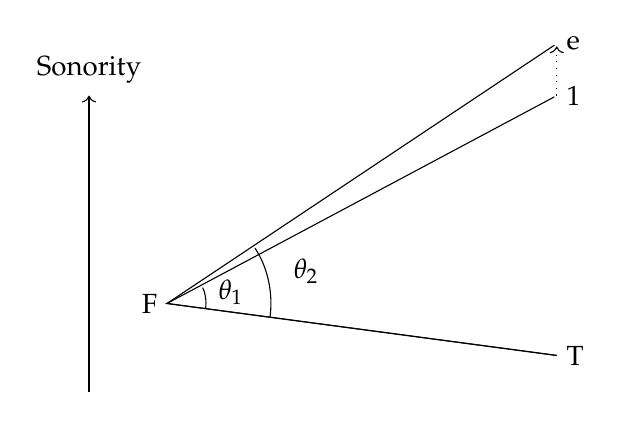
\begin{tikzpicture} [shorten >=1pt,scale=0.33]
                      \draw [<-] (-3,12) -- (-3, 0.5) ; % axis
                      \node at (-3, 13.0) {Sonority}; % axis label
					 % left diagram
    \coordinate (A) at (0,4); % pivot - C1 - F * 3
    \coordinate (B) at (15,2); % C2 - T * 3
    \coordinate (C) at (15,12); % V
    \coordinate (D) at (15,14); % V2
    \draw (B) -- (A) -- (C);
    \draw (B) -- (A) -- (D);
	\tkzMarkAngle[size=1.5](B,A,C);
	\tkzLabelAngle[pos=2.5](B,A,C){$\theta_1$};
	\tkzMarkAngle[size=4](B,A,D);
	\tkzLabelAngle[pos=5.5](B,A,D){$\theta_2$};
    
    \node[left] at  (A) {F}; 
    \node[right] at (B) {T};
    \node[right] at (C) {\textipa{1}};
    \node[right] at (D) {\textipa{e}};
    \draw [->,dotted] (C) -- (D);
\end{tikzpicture} 
\end{center}

This cannot be the whole story as other vowels are permitted to be epenthetic as well, for example [a], a low and extremely sonorous vowel, is epenthetic in several languages \citep{lombardi.2002}. Still, sonority contour faithfulness can potentially explain a large swathe of the epenthetic vowel typology.

\bigskip

To conclude this section, we see that the possible applications of sonority contour faithfulness are broad, encompassing many sonority-sensitive phonological processes. However, to pin down the exact parameters of the metric require more work.


\section{Conclusion} \label{conclusion}

In this paper, I argued for sonority contour faithfulness being the right way to analyse sonority-driven epenthesis, giving case studies in Irish and Chaha as examples. I additionally proposed that sonority contour distance should be computed by a metric that obeys two desiderata:

\ex. Desiderata for a sonority contour faithfulness metric 
     \a. The more positive the gradient of the sonority contour from C\textsubscript{1} to C\textsubscript{2}, the smaller the faithfulness cost. 
     \b. For a given sonority distance between C\textsubscript{1} and C\textsubscript{2}, the more sonorous C\textsubscript{1} and C\textsubscript{2} are, the smaller the faithfulness cost.

Using {\sc Sonority Angle} as a concrete example of a metric that obeys these two desiderata, I showed that  a sonority contour faithfulness account based on {\sc Sonority Angle} worked better than a cluster markedness-based account of sonority-driven epenthesis in Irish. Firstly, the faithfulness-based analysis did not need separate constraints for heterosyllabic and coda clusters like Syllable Contact and Sonority Sequencing, which more economically accounted for the ``coincidence'' that the same clusters were allowed and disallowed in both syllabic contexts. Secondly, the markedness-based approach in Irish could not account for why obstruent-initial heterosyllabic and coda clusters are tolerated in Irish even though these should be more marked than sonorant-initial clusters under the two sonority-based markedness constraints.

In addition, compared to the {\sc *Dis} metric \citep{gouskova.2002} for measuring sonority distance in Syllable Contact and Sonority Sequencing, and the alternative sonority contour faithfulness metric {\sc Sonority Rise} \citep{flemming.2008}, {\sc Sonority Angle} made the correct predictions that nasal-voiceless stop and liquid-voiceless stop clusters should be the hardest to epenthesise into in Irish, and the prediction that liquid-nasal clusters should be the most susceptible to epenthesis out of the falling sonority clusters in Chaha.

In Chaha, we saw more generally that the family of {\sc Ident(Son$\measuredangle$)}$<$n constraints, coupled with standard syllabic markedness constraints and alignment/anchor constraints preferring epenthesis on the left or right, yielded the complex and variable system of epenthesis positioning in the language with only one error in predictions, making it comparably successful to the existing Syllable Contact-based analysis by \cite{rose.2000}.

{\sc Sonority Angle} was offered here as a concrete instance of the class of metrics that conform to the two desiderata. In $\S$\ref{issues}, I discussed several issues regarding the assumptions that need to be incorporated into its formulation. More perceptual experiments and cross-linguistic investigation of sonority-driven epenthesis needs to be done to pin down the specifics of the metric. In addition, I discussed two other sonority-based phenomena that may shed additional light on the true nature of sonority contour faithfulness.

\section*{Acknowledgments}

I would like to thank Donca Steriade, Adam Albright, Michael Kenstowicz, Edward Flemming, Suyeon Yun, Gretchen Kern, Hrayr Khanjian, and audiences at the MIT Phonology Circle and Manchester Phonology Meeting for valuable feedback on this project. This material is based upon work supported by the National Science Foundation Graduate Research Fellowship Program under Grant No. 1122374.

\bibliographystyle{apalike}
\bibliography{sonangle}


\end{document}
